\documentclass[../Thesis.tex]{subfiles}
\begin{document}
\section{Cài đặt server side open source Canvas LMS trên Google Cloud}
    Trong phần này, chúng ta sẽ trình bày quá trình cài đặt server side open source Canvas LMS trên nền tảng Google Cloud. Canvas LMS được xây dựng bằng ngôn ngữ Ruby và được triển khai trên máy chủ web.
    \subsection{Chuẩn bị môi trường}
        \begin{enumerate}
            \item Đăng ký tài khoản Google Cloud: Truy cập vào trang web của Google Cloud và tạo một tài khoản nếu bạn chưa có. Sau khi hoàn thành việc đăng ký, bạn sẽ được chuyển đến bảng điều khiển Google Cloud.
            \begin{figure}[hbt!]
                \centering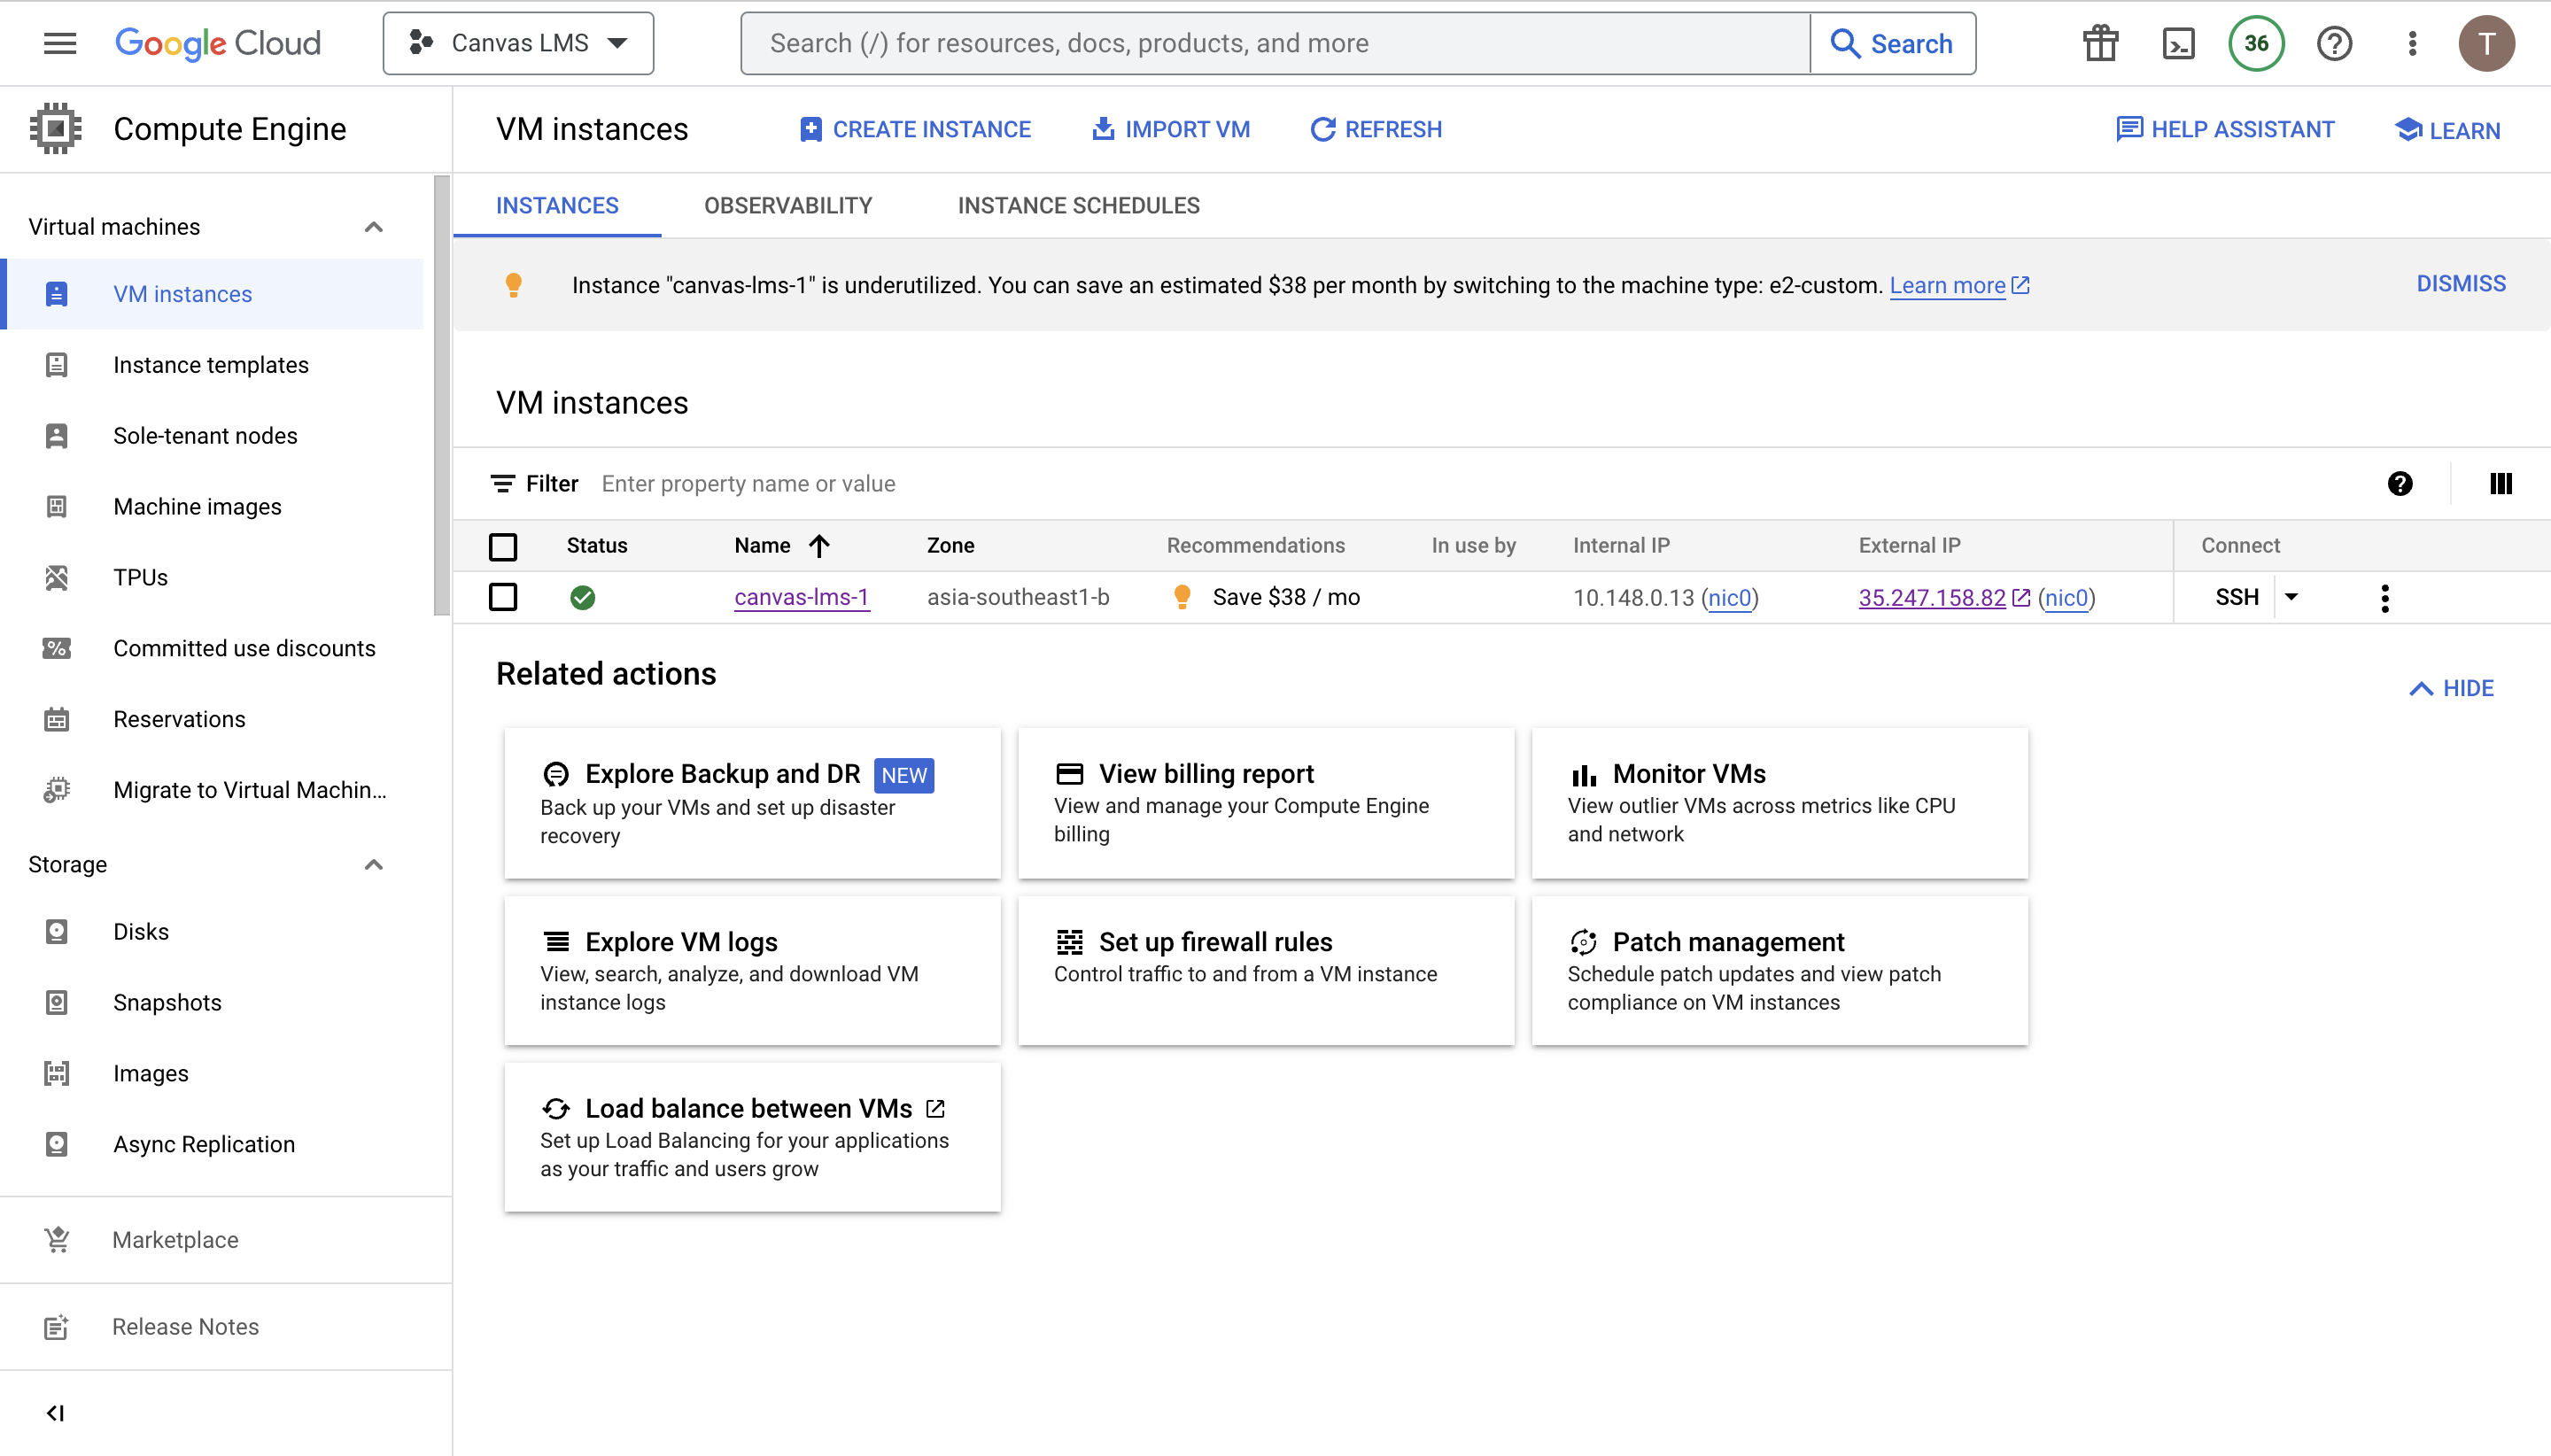
\includegraphics[width=300pt, height=200pt]{1-google-cloud-console}
                \caption{Màn hình Google Cloud Console}
                \label{fig:google-cloud-console}
            \end{figure}
            \FloatBarrier
            \item Tạo máy ảo: Trên bảng điều khiển Google Cloud, chúng ta sẽ thực hiện việc tạo một máy ảo để chạy Canvas LMS. Để tạo máy ảo, chúng ta nhấp vào mục "Compute Engine" trên bảng điều khiển. Tiếp theo, chọn "Máy ảo" và nhấp vào nút "Tạo máy ảo".

            Trong trang tạo máy ảo, bạn sẽ cần cung cấp các thông tin sau:
            \begin{itemize}
                \item Tên máy ảo: Đặt tên cho máy ảo của bạn để dễ nhận biết.
                \item Kích thước máy ảo: Chọn kích thước máy ảo phù hợp với yêu cầu của bạn, bao gồm số lượng bộ nhớ RAM và vCPU.
                \item Vùng địa lý: Chọn vùng địa lý gần với địa điểm của bạn để đảm bảo tốc độ truy cập nhanh nhất.
                \item Firewall: Cấu hình các quy tắc tường lửa cho phép truy cập vào máy ảo.
            \end{itemize}
            \begin{figure}[hbt!]
                \centering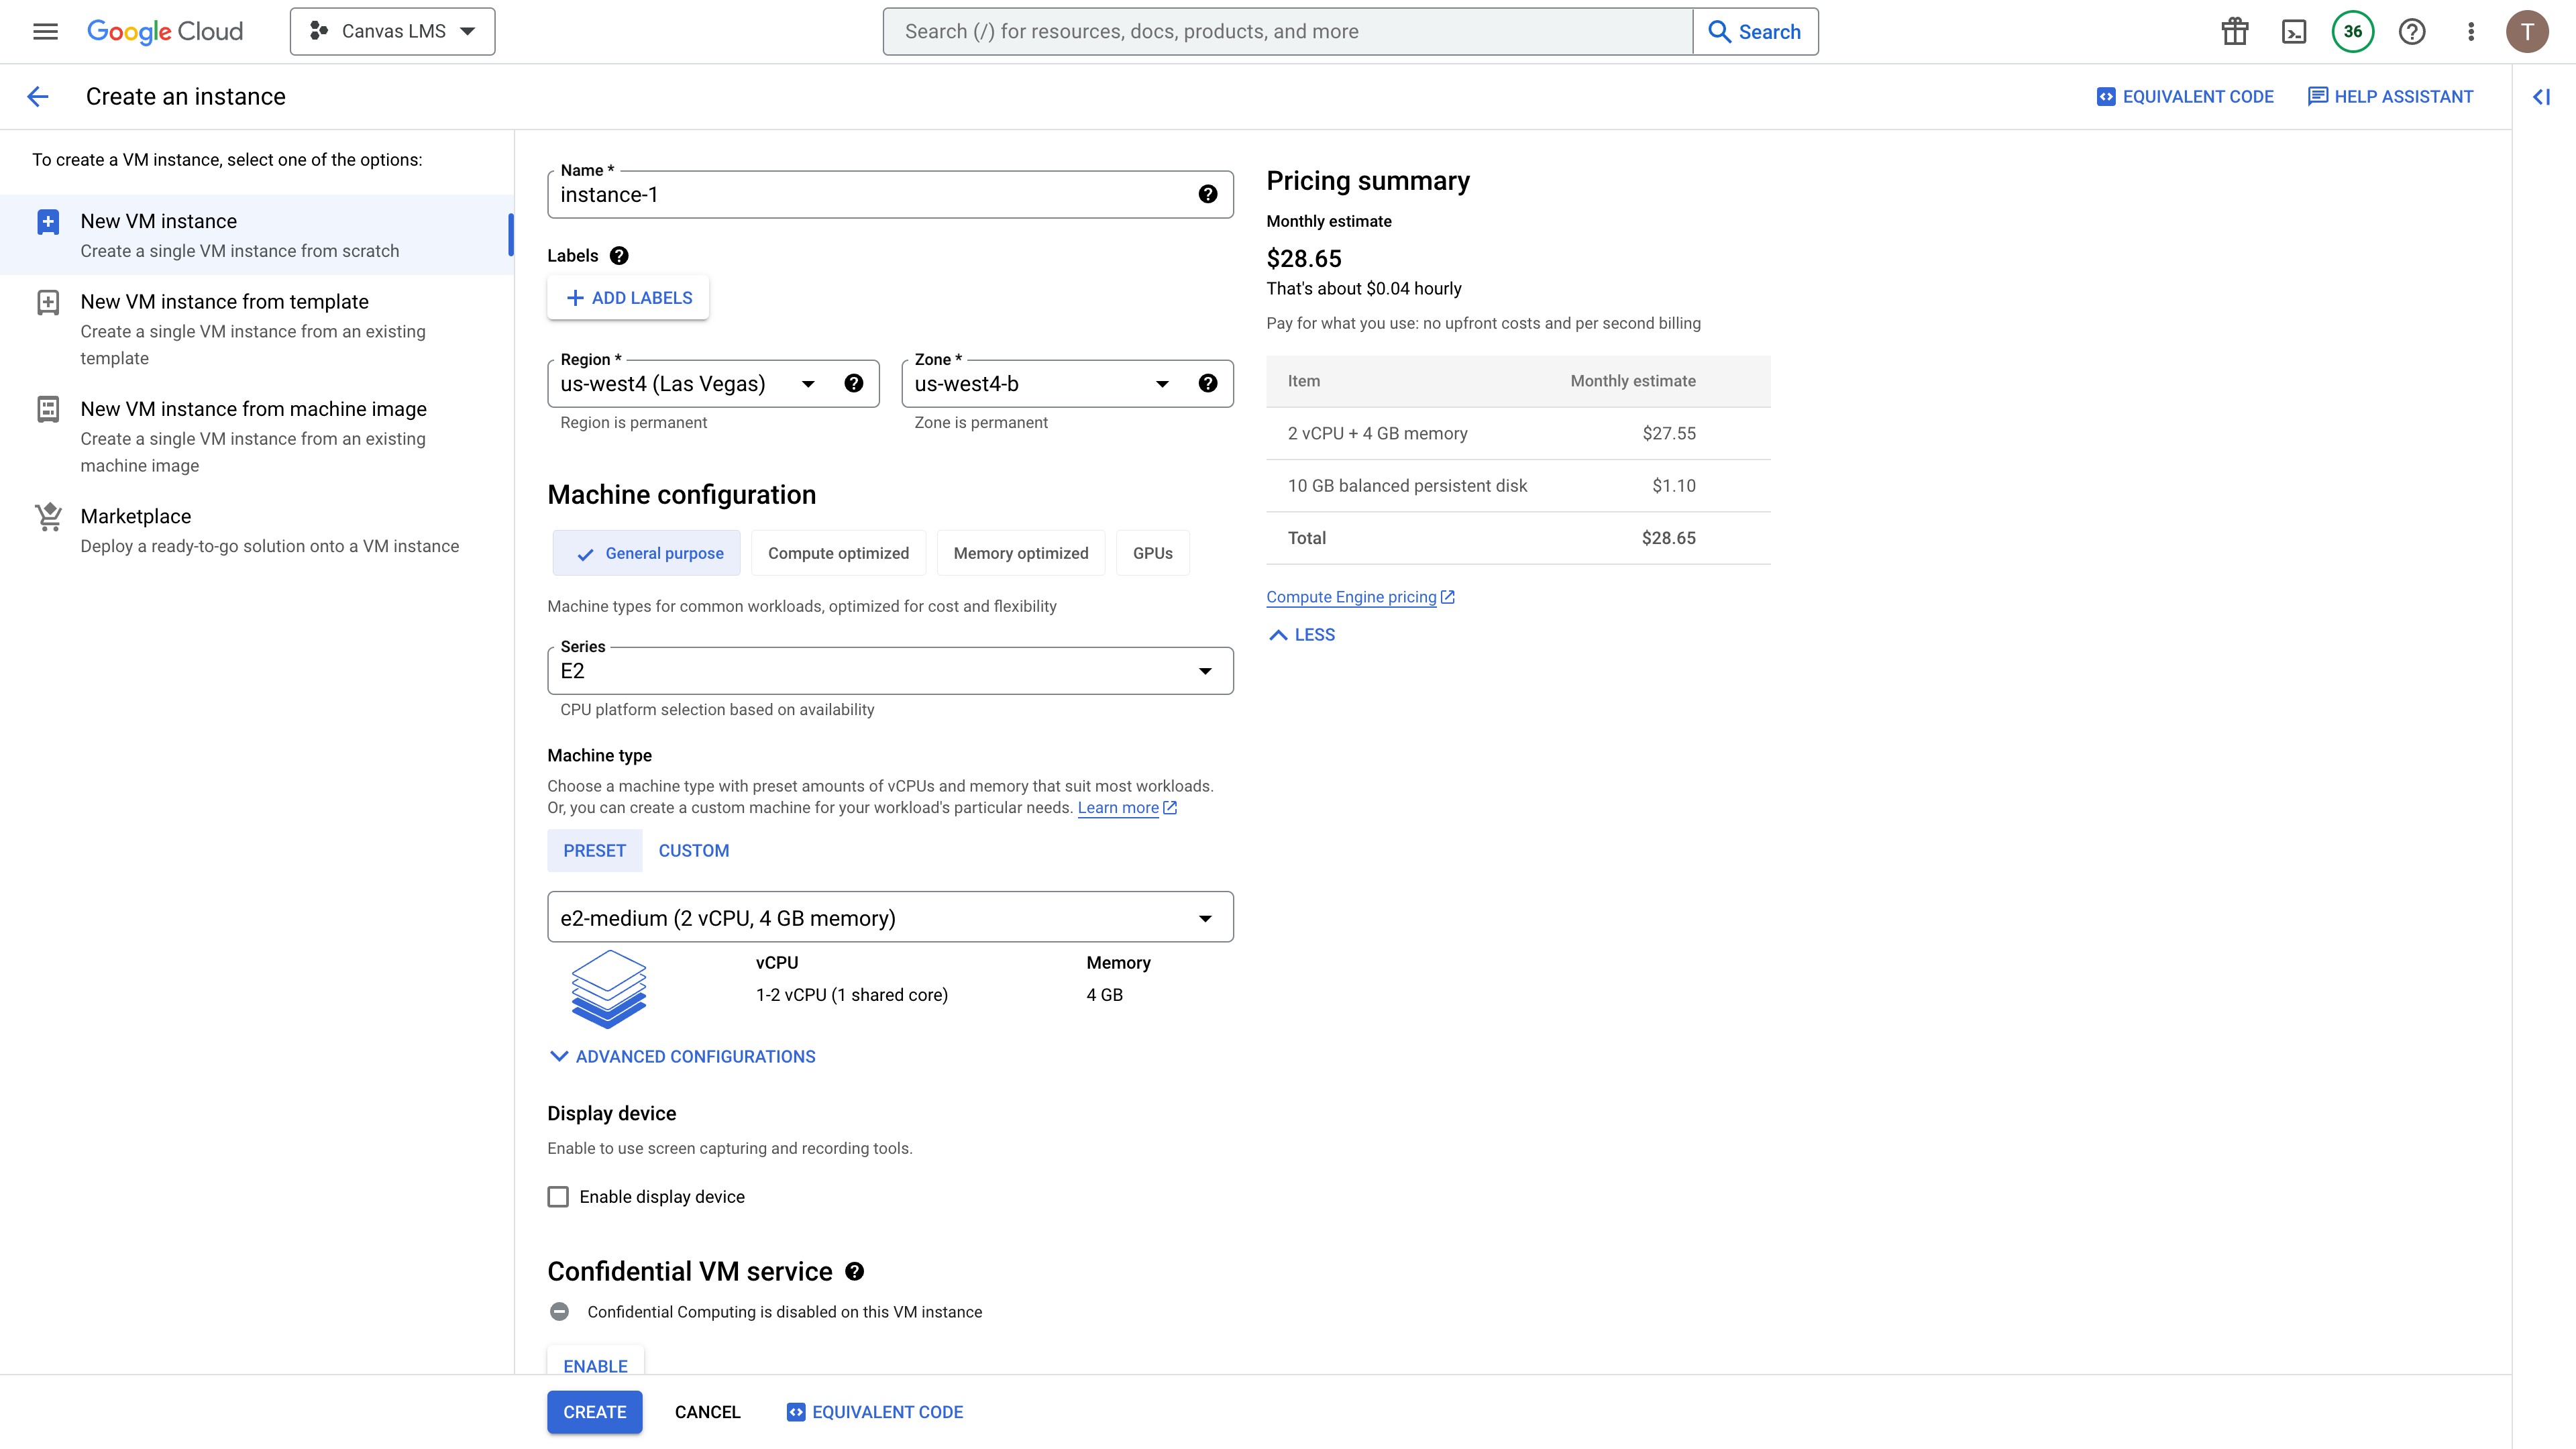
\includegraphics[width=300pt, height=200pt]{google-create-instance}
                \caption{Màn hình tạo máy ảo}
                \label{fig:google-create-instance}
            \end{figure}
            \FloatBarrier

            \item Cấu hình mạng: Đảm bảo rằng máy ảo của bạn được cấu hình để có địa chỉ IP công cộng và có quyền truy cập Internet. Điều này sẽ đảm bảo rằng máy ảo có thể truy cập vào các tài nguyên cần thiết và có thể phục vụ các yêu cầu từ người dùng.

            Trên bảng điều khiển Google Cloud, chúng ta có thể cấu hình các thiết lập mạng cho máy ảo bằng cách điều hướng đến mục "Network" hoặc "Mạng" trên bảng điều khiển.
            
            Ở đây, chúng ta có thể thực hiện các tác vụ như gán địa chỉ IP công cộng, tạo và quản lý các quy tắc tường lửa, cấu hình phân giải tên miền và nhiều hơn nữa.

            \begin{figure}[hbt!]
                \centering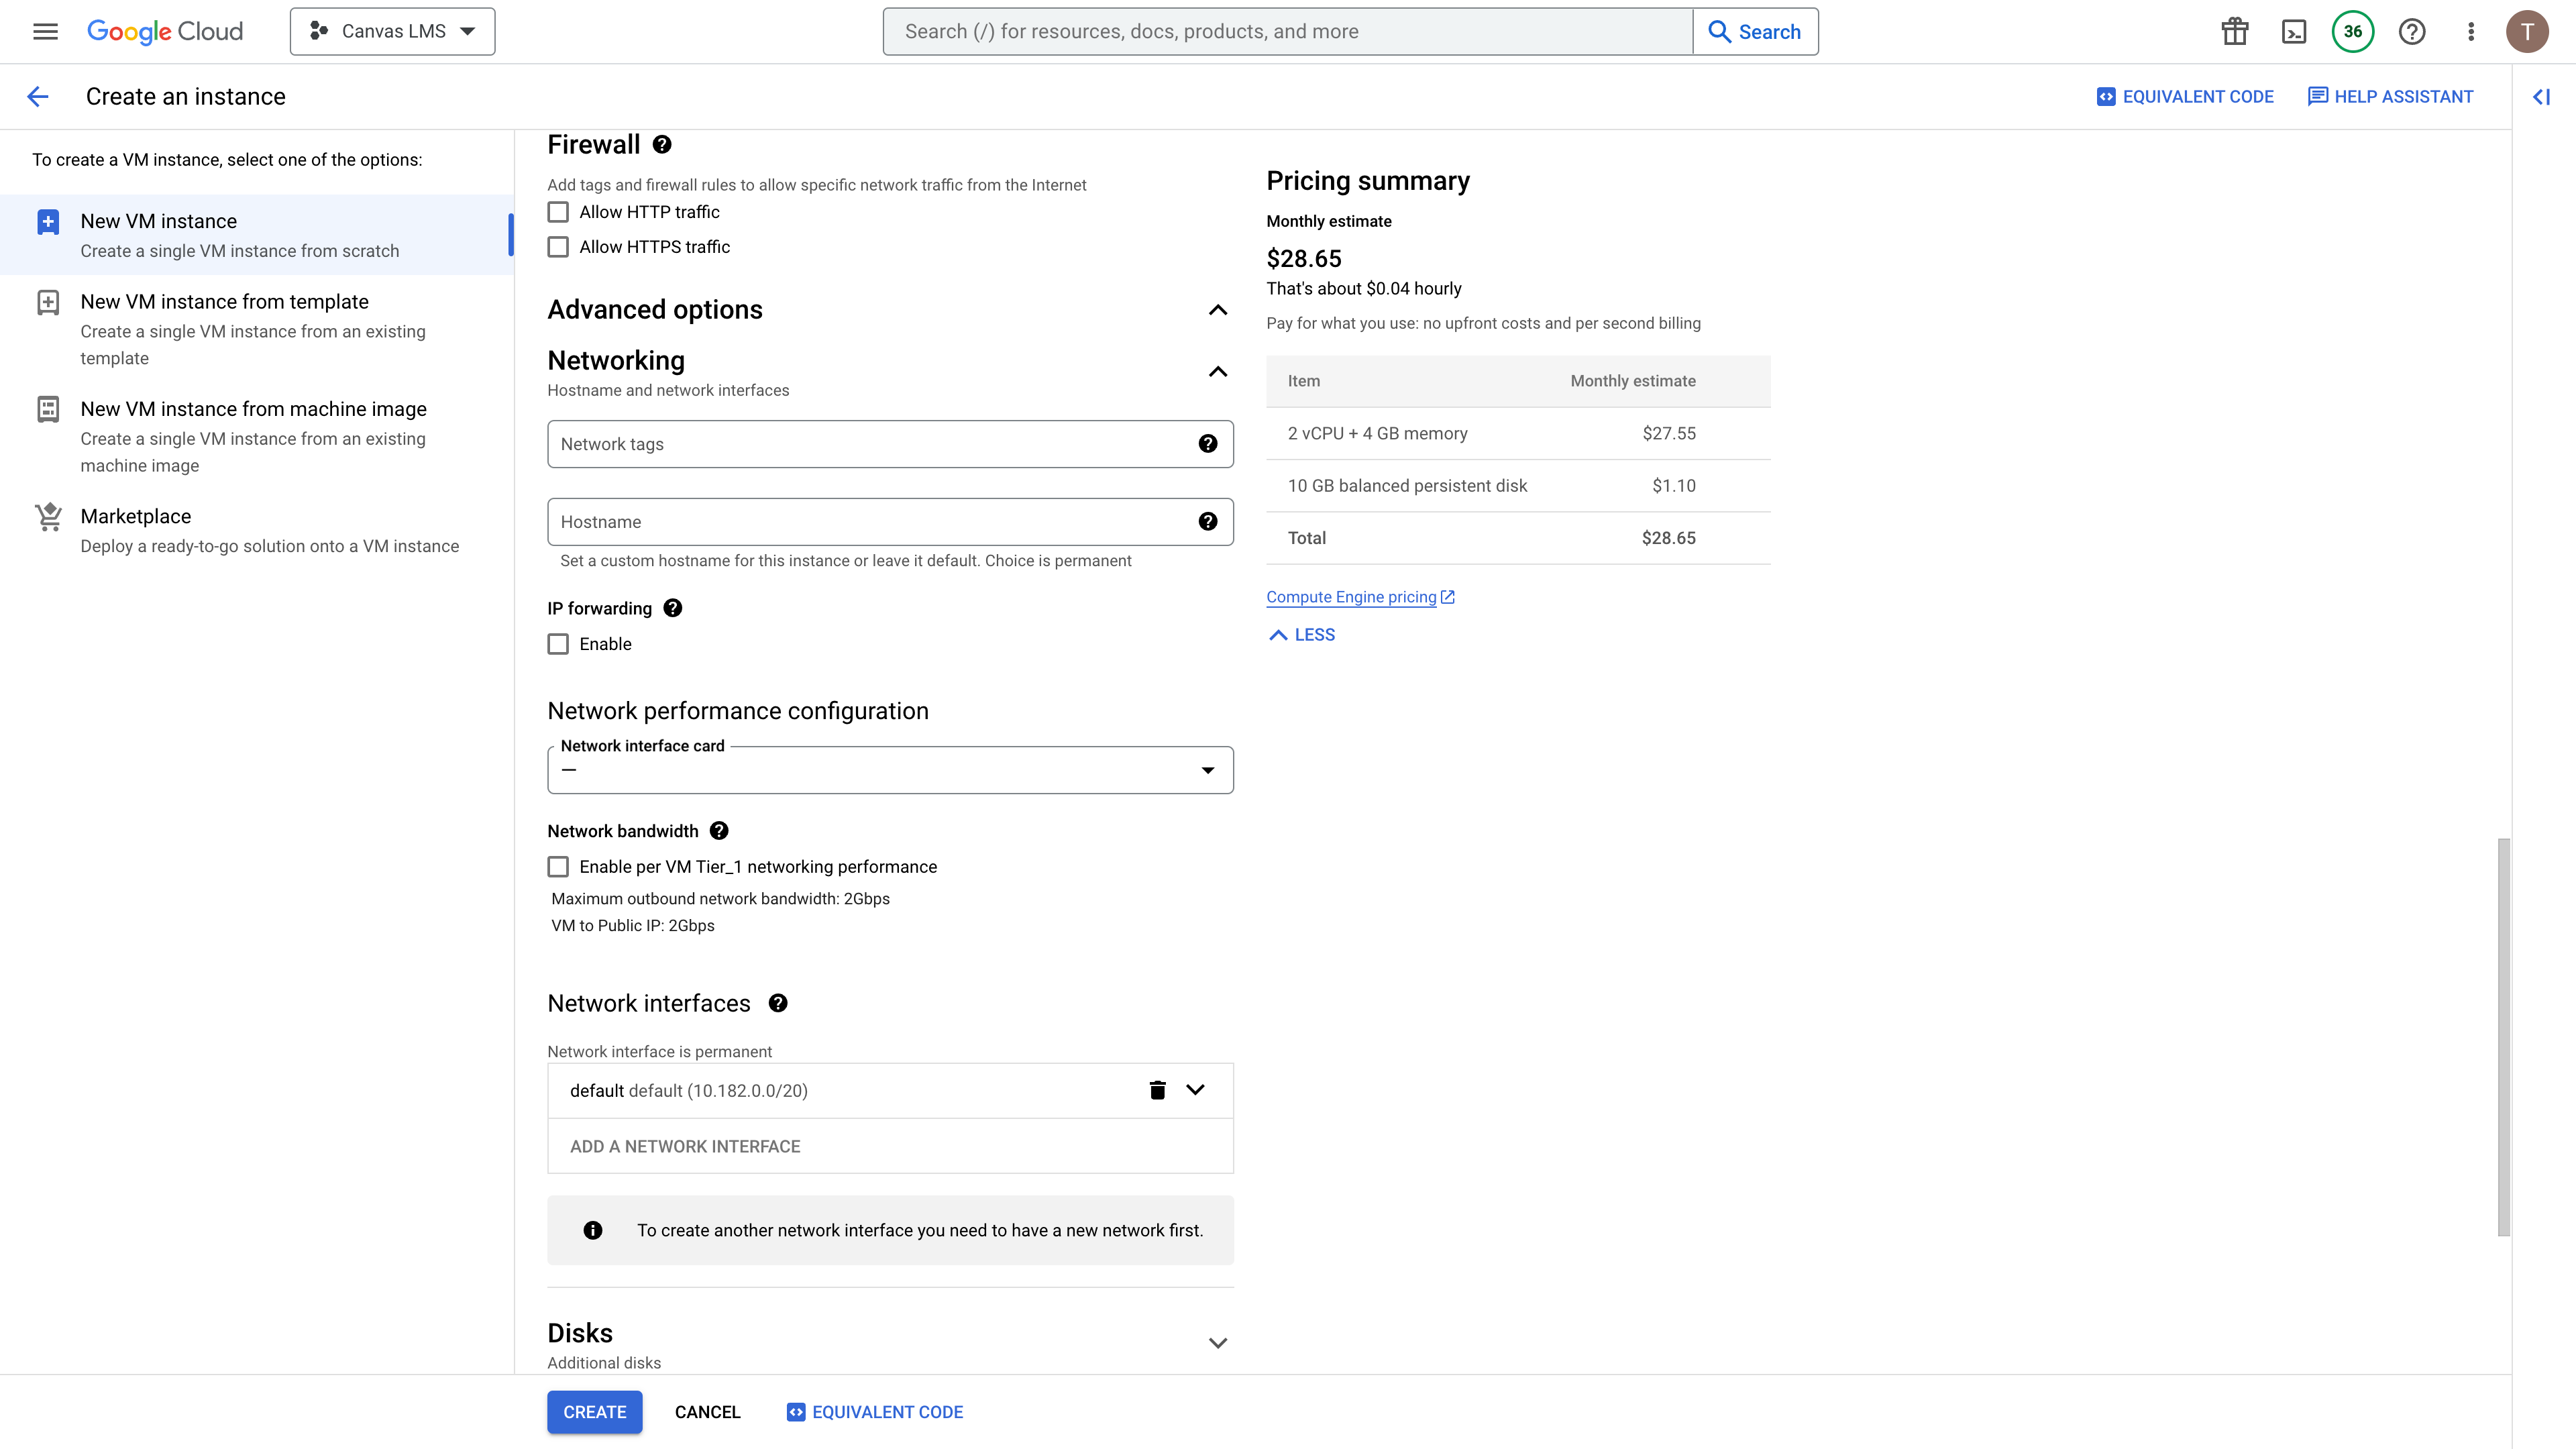
\includegraphics[width=300pt, height=200pt]{google-network}
                \caption{Cài đặt mạng cho máy ảo}
                \label{fig:google-network}
            \end{figure}
            \FloatBarrier

            \item Cài đặt và cấu hình Canvas LMS: Sau khi đã chuẩn bị môi trường, chúng ta có thể tiến hành cài đặt và cấu hình Canvas LMS trên máy ảo. Quá trình này bao gồm cài đặt Ruby, PostgreSQL, các gói phụ thuộc và mã nguồn Canvas LMS.

            Để cài đặt và cấu hình Canvas LMS, chúng ta sẽ sử dụng các lệnh và tệp cấu hình được cung cấp trong mã nguồn của Canvas LMS. Quá trình này yêu cầu kiến thức về quản lý máy chủ và cài đặt ứng dụng web.
            
            Sau khi cài đặt và cấu hình thành công, chúng ta sẽ có một môi trường Canvas LMS hoạt động trên máy ảo của chúng ta trên Google Cloud.
        \end{enumerate}
    \subsection{Cài đặt Canvas LMS}
        \begin{enumerate}
            \item Cài đặt Ruby: Canvas LMS yêu cầu phiên bản Ruby 2.7.3. Để cài đặt phiên bản này, chúng ta sẽ sử dụng RVM (Ruby Version Manager). RVM là một công cụ quản lý phiên bản Ruby cho phép chúng ta cài đặt nhiều phiên bản Ruby trên cùng một máy tính.

            Để cài đặt RVM, chúng ta sẽ sử dụng lệnh sau:
            \begin{lstlisting}[language=bash]
                $ curl -sSL https://rvm.io/mpapis.asc | gpg --import -
                $ curl -sSL https://get.rvm.io | bash -s stable
            \end{lstlisting}

            Sau khi cài đặt RVM, chúng ta sẽ cài đặt phiên bản Ruby 2.7.3 bằng lệnh sau:
            \begin{lstlisting}[language=bash]
                $ rvm install 2.7.3
            \end{lstlisting}

            \item Cài đặt PostgreSQL: Canvas LMS yêu cầu phiên bản PostgreSQL 9.5. Để cài đặt phiên bản này, chúng ta sẽ sử dụng các lệnh sau:
            \begin{lstlisting}[language=bash]
                $ sudo apt-get update
                $ sudo apt-get install postgresql postgresql-contrib
            \end{lstlisting}

            Sau khi cài đặt PostgreSQL, chúng ta sẽ tạo một người dùng và một cơ sở dữ liệu cho Canvas LMS. Để làm điều này, chúng ta sẽ sử dụng các lệnh sau:
            \begin{lstlisting}[language=bash]
                $ sudo -u postgres createuser canvas --no-createdb --no-superuser --no-createrole --pwprompt
                $ sudo -u postgres createdb canvas_production --owner=canvas
            \end{lstlisting}

            \item Cài đặt các gói phụ thuộc: Canvas LMS yêu cầu một số gói phụ thuộc để có thể hoạt động. Để cài đặt các gói phụ thuộc này, chúng ta sẽ sử dụng các lệnh sau:
            \begin{lstlisting}[language=bash]
                $ sudo apt-get install git-core curl zlib1g-dev build-essential libssl-dev libreadline-dev libyaml-dev libsqlite3-dev sqlite3 libxml2-dev libxslt1-dev libcurl4-openssl-dev software-properties-common libffi-dev
            \end{lstlisting}

            \item Cài đặt mã nguồn Canvas LMS: Sau khi đã cài đặt các gói phụ thuộc, chúng ta sẽ tiến hành cài đặt mã nguồn Canvas LMS. Để làm điều này, chúng ta sẽ sử dụng các lệnh sau:
            \begin{lstlisting}[language=bash]
                $ cd ~
                $ git clone https://github.com/instructure/canvas-lms.git canvas
                $ cd canvas
                $ git checkout prod
                $ sudo mkdir -p /var/canvas
                $ sudo chown -R $USER /var/canvas
                $ cp -av . /var/canvas
            \end{lstlisting}

            \item Càu đặt yarn sau khi đã cài đặt mã nguồn Canvas LMS: Canvas LMS yêu cầu yarn để có thể hoạt động. Để cài đặt yarn, chúng ta sẽ sử dụng các lệnh sau:
            \begin{lstlisting}[language=bash]
                $ curl -sS https://dl.yarnpkg.com/debian/pubkey.gpg | sudo apt-key add -
                $ echo "deb https://dl.yarnpkg.com/debian/ stable main" | sudo tee /etc/apt/sources.list.d/yarn.list
                $ sudo apt-get update
                $ sudo apt-get install yarn
            \end{lstlisting}

            \item Cài đặt các gói phụ thuộc của Canvas LMS: Sau khi đã cài đặt yarn, chúng ta sẽ tiến hành cài đặt các gói phụ thuộc của Canvas LMS. Để làm điều này, chúng ta sẽ sử dụng các lệnh sau:
            \begin{lstlisting}[language=bash]
                $ cd /var/canvas
                $ bundle config set path 'vendor/bundle'
                $ yarn install
            \end{lstlisting}



            \item Cấu hình Canvas LMS: Sau khi đã cài đặt yarn, chúng ta sẽ tiến hành cấu hình Canvas LMS. Để làm điều này, chúng ta sẽ sử dụng các lệnh sau:
            \begin{lstlisting}[language=bash]
                $ cp config/database.yml.example config/database.yml
                $ nano config/database.yml
                $ bundle exec rake canvas:compile_assets
            \end{lstlisting}

            \item Cấu hình Apache: Sau khi đã cấu hình Canvas LMS, chúng ta sẽ tiến hành cấu hình Apache. Để làm điều này, chúng ta sẽ sử dụng các lệnh sau:

            Đầu tiên, chúng ta sẽ cài đặt Apache bằng lệnh sau:
            \begin{lstlisting}[language=bash]
                $ sudo apt-get install apache2
                $ sudo apt-get install -y libapache2-mod-passenger
            \end{lstlisting}

            Sau đó, chúng ta sẽ cấu hình Apache bằng lệnh sau:
            \begin{lstlisting}[language=bash]
                $ sudo nano /etc/apache2/sites-available/canvas.conf
            \end{lstlisting}

            Trong file cấu hình này, chúng ta sẽ thêm các dòng sau:
            \begin{lstlisting}[language=bash]
                <VirtualHost *:80>
                    ServerName 35.247.158.82
                    ServerAlias canvasfiles.example.com
                    ServerAdmin brad@sandbox84e1f41fa65f4f75941861cde77b288a.mailgun.org
                    DocumentRoot /var/canvas/public
                    RewriteEngine On
                    RewriteCond %{HTTP:X-Forwarded-Proto} !=https
                    RewriteCond %{REQUEST_URI} !^/health_check
                    RewriteRule (.*) https://%{HTTP_HOST}%{REQUEST_URI} [L]
                    ErrorLog /var/log/apache2/canvas_errors.log
                    LogLevel warn
                    CustomLog /var/log/apache2/canvas_access.log combined
                    SetEnv RAILS_ENV production
                    <Directory /var/canvas/public>
                        Options All
                        AllowOverride All
                        Require all granted
                    </Directory>
                </VirtualHost>
                    # If you are only serving HTTP behind a HTTPS-terminating load balancer, skip the next VirtualHost
                <VirtualHost *:443>
                    ServerName 35.247.158.82
                    ServerAlias canvasfiles.example.com
                    ServerAdmin brad@sandbox84e1f41fa65f4f75941861cde77b288a.mailgun.org
                    DocumentRoot /var/canvas/public
                    ErrorLog /var/log/apache2/canvas_errors.log
                    LogLevel warn
                    CustomLog /var/log/apache2/canvas_ssl_access.log combined
                    SSLEngine on
                    BrowserMatch "MSIE [17-9]" ssl-unclean-shutdown
                    # the following ssl certificate files are generated for you from the ssl-cert package.
                    SSLCertificateFile /etc/ssl/certs/ssl-cert-snakeoil.pem
                    SSLCertificateKeyFile /etc/ssl/private/ssl-cert-snakeoil.key
                    SetEnv RAILS_ENV production
                    <Directory /var/canvas/public>
                        Options All
                        AllowOverride All
                        Require all granted
                    </Directory>
                </VirtualHost>
            \end{lstlisting}

            Sau đó, chúng ta sẽ cấu hình Apache bằng lệnh sau:
            \begin{lstlisting}[language=bash]
                $ sudo a2enmod ssl
                $ sudo a2enmod headers
                $ sudo a2ensite canvas
                $ sudo a2enmod rewrite
                $ sudo a2dissite 000-default
                $ sudo service apache2 restart
            \end{lstlisting}

            \item Cấu hình Canvas LMS: Sau khi đã cấu hình Apache, chúng ta sẽ tiến hành cấu hình Canvas LMS. Để làm điều này, chúng ta sẽ sử dụng các lệnh sau:
            
            Đầu tiên, chúng ta sẽ cấu hình Canvas LMS bằng lệnh sau:
            \begin{lstlisting}[language=bash]
                $ cp config/outgoing_mail.yml.example config/outgoing_mail.yml
                $ nano config/outgoing_mail.yml
            \end{lstlisting}

            Trong file cấu hình này, chúng ta sẽ thêm các dòng sau:
            \begin{lstlisting}[language=bash]
                production:
                    address: "smtp.mailgun.org"
                    port: "587"
                    user_name: "postmaster@sandbox84e1f41fa65f4f75941861cde77b288a.mailgun.org"
                    password: "thuongkhung120"
                    authentication: "login" # plain, login, or cram_md5
                    domain: "sandbox84e1f41fa65f4f75941861cde77b288a.mailgun.org"
                    outgoing_address: "thuongkhungvu@gmail.com"
                    default_name: "Thuy Loi University"
            \end{lstlisting}

            Sau đó, chúng ta sẽ cấu hình Canvas LMS bằng lệnh sau:
            \begin{lstlisting}[language=bash]
                $ cp config/domain.yml.example config/domain.yml
                $ nano config/domain.yml
            \end{lstlisting}

            Trong file cấu hình này, chúng ta sẽ thêm các dòng sau:
            \begin{lstlisting}[language=bash]
                production:
                    domain: "35.247.158.82"
                    ssl: true
            \end{lstlisting}

            Sau đó, chúng ta sẽ cấu hình Canvas LMS bằng lệnh sau:
            \begin{lstlisting}[language=bash]
                $ cp config/security.yml.example config/security.yml
                $ nano config/security.yml
            \end{lstlisting}

            Trong file cấu hình này, chúng ta sẽ thêm các dòng sau:
            \begin{lstlisting}[language=bash]
                production: &default
                    encryption_key: jsn2hsydandsu299374msdmcbusnk213nfdu2
            \end{lstlisting}

            Sau đó, chúng ta sẽ cấu hình Canvas LMS bằng lệnh sau:
            \begin{lstlisting}[language=bash]
                $ cp config/cache_store.yml.example config/cache_store.yml
                $ nano config/cache_store.yml
            \end{lstlisting}

            Trong file cấu hình này, chúng ta sẽ thêm các dòng sau:
            \begin{lstlisting}[language=bash]
                production:
                    cache_store: redis_cache_store
            \end{lstlisting}

            Sau đó, chúng ta sẽ cấu hình Canvas LMS bằng lệnh sau:
            \begin{lstlisting}[language=bash]
                $ cp config/redis.yml.example config/redis.yml
                $ nano config/redis.yml
            \end{lstlisting}

            Trong file cấu hình này, chúng ta sẽ thêm các dòng sau:
            \begin{lstlisting}[language=bash]
                production:
                    servers:
                    - redis://localhost
            \end{lstlisting}

            Sau khi đã cài đặt xong các gói cần thiết, chúng ta sẽ tiến hành cài đặt Canvas LMS bằng lệnh sau:
            \begin{lstlisting}[language=bash]
                $ bundle install --deployment --without development test postgres
                $ bundle exec rake db:create
                $ bundle exec rake db:initial_setup
                $ bundle exec rake canvas:compile_assets
            \end{lstlisting}

            Sau khi đã cài đặt xong Canvas LMS, chúng ta sẽ tiến hành cấu hình Canvas LMS bằng lệnh sau:
            \begin{lstlisting}[language=bash]
                $ cp config/production.example.yml config/production.yml
                $ nano config/production.yml
            \end{lstlisting}

            Trong file cấu hình này, chúng ta sẽ thêm các dòng sau:
            \begin{lstlisting}[language=bash]
                production:
                    domain: "35.247.158.82"
                    ssl: true
            \end{lstlisting}

            Sau khi đã cấu hình xong Canvas LMS, chúng ta sẽ tiến hành cài đặt Canvas LMS bằng lệnh sau:
            \begin{lstlisting}[language=bash]
                $ bundle exec rake canvas:compile_assets
            \end{lstlisting}

        Sau khi hoàn thành cài đặt, chúng ta sẽ tiến hành khởi động lại Canvas LMS bằng lệnh sau:
            \begin{lstlisting}[language=bash]
                $ sudo /etc/init.d/apache2 restart
            \end{lstlisting}

            Sau khi khởi động lại Canvas LMS, chúng ta sẽ truy cập vào địa chỉ \url{http://35.247.158.82} để kiểm tra kết quả.
        \end{enumerate}

\section{Xây dựng phần giao diện cho hệ thống}
\label{subsec:xay-dung-giao-dien}

    Trong phiên bản hiện tại của hệ thống, tôi đã xây dựng và triển khai một số phần quan trọng nhằm đáp ứng các yêu cầu và chức năng cơ bản của một nền tảng học trực tuyến. Dưới đây là mô tả chi tiết về các phần đã được xây dựng:

    \begin{itemize}
        \item Landing page:
            \begin{itemize}
                \item Trang landing page được thiết kế để hiển thị các khoá học công khai, giới thiệu về nền tảng và thu hút sự quan tâm của người dùng.
                \item Trang này cung cấp một giao diện hấp dẫn với thông tin tóm tắt về các khoá học và mô tả về chương trình học.
            \end{itemize}
        \item Đăng nhập:
            \begin{itemize}
                \item Phần đăng nhập cho phép người dùng truy cập vào tài khoản cá nhân của mình thông qua việc nhập thông tin đăng nhập.
                \item Tôi đã tạo giao diện đơn giản và bảo mật để đảm bảo quyền riêng tư và truy cập an toàn cho người dùng.
            \end{itemize}
    
        \item Hiển thị khoá học:
            \begin{itemize}
                \item Trang hiển thị khoá học cung cấp một giao diện dễ sử dụng và thân thiện cho người dùng để tìm kiếm, xem và tham gia các khoá học.
                \item Các khoá học được hiển thị dưới dạng danh sách hoặc lưới, kèm theo thông tin chi tiết về mô tả, giảng viên, thời gian học, và điểm số.
            \end{itemize}
        \item Quản lý khoá học:
            \begin{itemize}
                \item Tôi đã phát triển các chức năng quản lý khoá học cho giảng viên, cho phép họ thêm, sửa đổi và xoá các khoá học một cách dễ dàng.
                \item Giảng viên có quyền quản lý thông tin, tài liệu, bài tập và câu hỏi kiểm tra trong khoá học của mình.
            \end{itemize}
   
        \item Quản lý bài tập:
            \begin{itemize}
                \item Phần quản lý bài tập cho phép giảng viên thêm, sửa đổi và xoá bài tập trong khoá học.
                \item Giảng viên có thể thiết lập các thông số như tiêu đề, mô tả, ngày hết hạn, trọng số, và điểm số cho mỗi bài tập.
            \end{itemize}
        \item Quản lý câu hỏi kiểm tra:
            \begin{itemize}
                \item Tôi đã tạo chức năng cho giảng viên để quản lý câu hỏi kiểm tra trong khoá học.
                \item Giảng viên có thể thêm, sửa đổi và xoá câu hỏi kiểm tra, và cũng có thể thiết lập điểm số cho từng câu hỏi.
            \end{itemize}
        \item Hiển thị điểm:
            \begin{itemize}
                \item Trang hiển thị điểm cung cấp một cái nhìn tổng quan về kết quả học tập của người dùng.
                \item Phần điểm số đã được chỉnh sửa để phù hợp hơn cho môi trường ở Việt Nam. Hiện tại app cho phép thiết lập 2 trọng số là trọng số của nhóm bài tập và trọng số của bài tập, tự đó hệ thống sẽ tự động tính điểm cho người dùng.
            \end{itemize}
        \item Lịch hiển thị sự kiện:
            \begin{itemize}
                \item Phần lịch hiển thị các sự kiện giúp người dùng có cái nhìn tổng quan về lịch trình học tập.
                \item Các sự kiện như buổi học, bài tập đến hạn, và các sự kiện quan trọng khác được hiển thị dễ nhìn và dễ sử dụng.
            \end{itemize}
        \item Tin nhắn:
            \begin{itemize}
                \item Tôi đã tạo chức năng gửi tin nhắn cho người dùng, cho phép họ giao tiếp và trao đổi thông tin với giảng viên và sinh viên khác.
                \item Người dùng có thể gửi tin nhắn riêng tư hoặc tham gia vào các cuộc thảo luận trong các nhóm học tập.
            \end{itemize}
        \item Cài đặt thông tin cá nhân:
            \begin{itemize}
                \item Phần cài đặt thông tin cá nhân cho phép người dùng quản lý và cập nhật thông tin cá nhân của mình.
                \item Người dùng có thể thay đổi thông tin liên hệ, mô tả bản thân, và các tùy chọn cá nhân khác theo nhu cầu của mình.
            \end{itemize}
    \end{itemize}
    
    \subsection{Chi tiết các chức năng}
        \subsubsection{Xây dựng giao diện chung}
        \label{subsubsec:xay-dung-giao-dien-chung}
            \begin{itemize}
                \item Phần landing page của hệ thống được thể hiện ở hình \ref{fig:landing-page}:
                \begin{figure}[hbt!]
                    \centering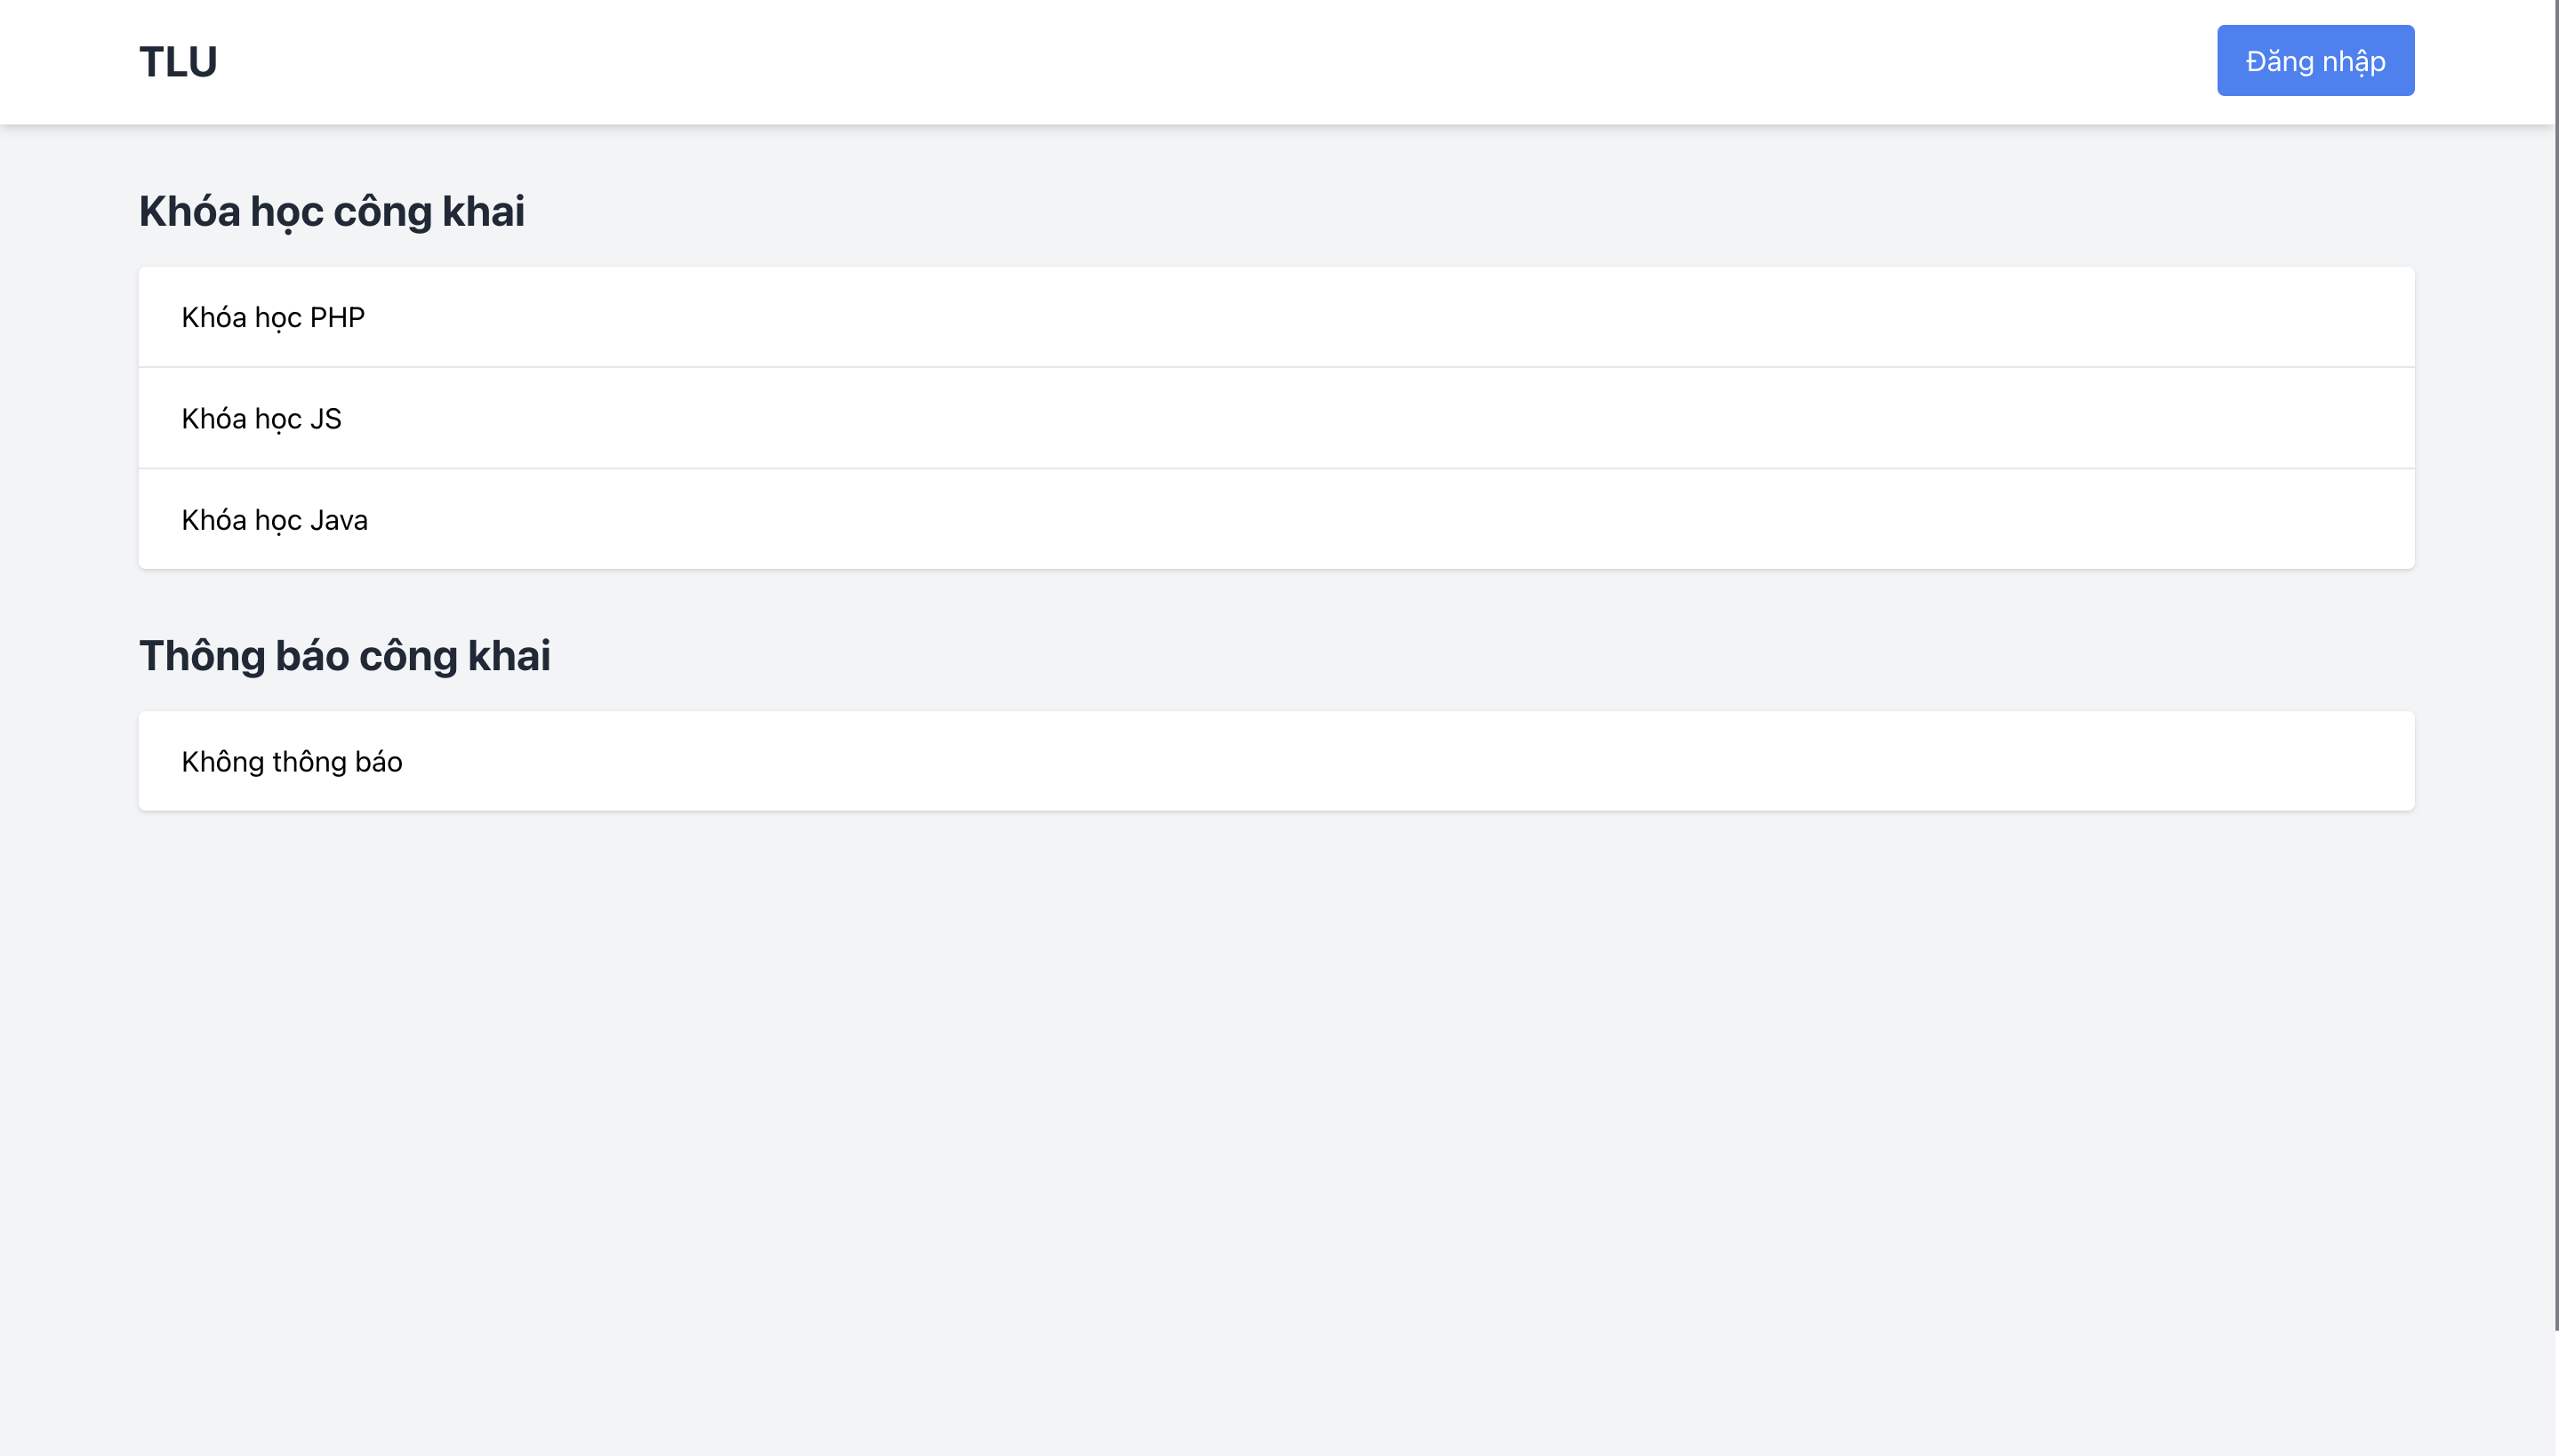
\includegraphics[width=300pt, height=200pt]{landing-page}
                    \caption{Màn hình landing page của hệ thống}
                    \label{fig:landing-page}
                \end{figure}
                \FloatBarrier

            \end{itemize}

        \subsubsection{Xây dựng giao diện cho phần quản trị viên}
        \label{subsubsec:xay-dung-giao-dien-admin}
        
            \begin{itemize}
                \item Phần đăng nhập của phần quản trị viên được thể hiện ở hình \ref{fig:dang-nhap-admin}:

                \begin{figure}[hbt!]
                    \centering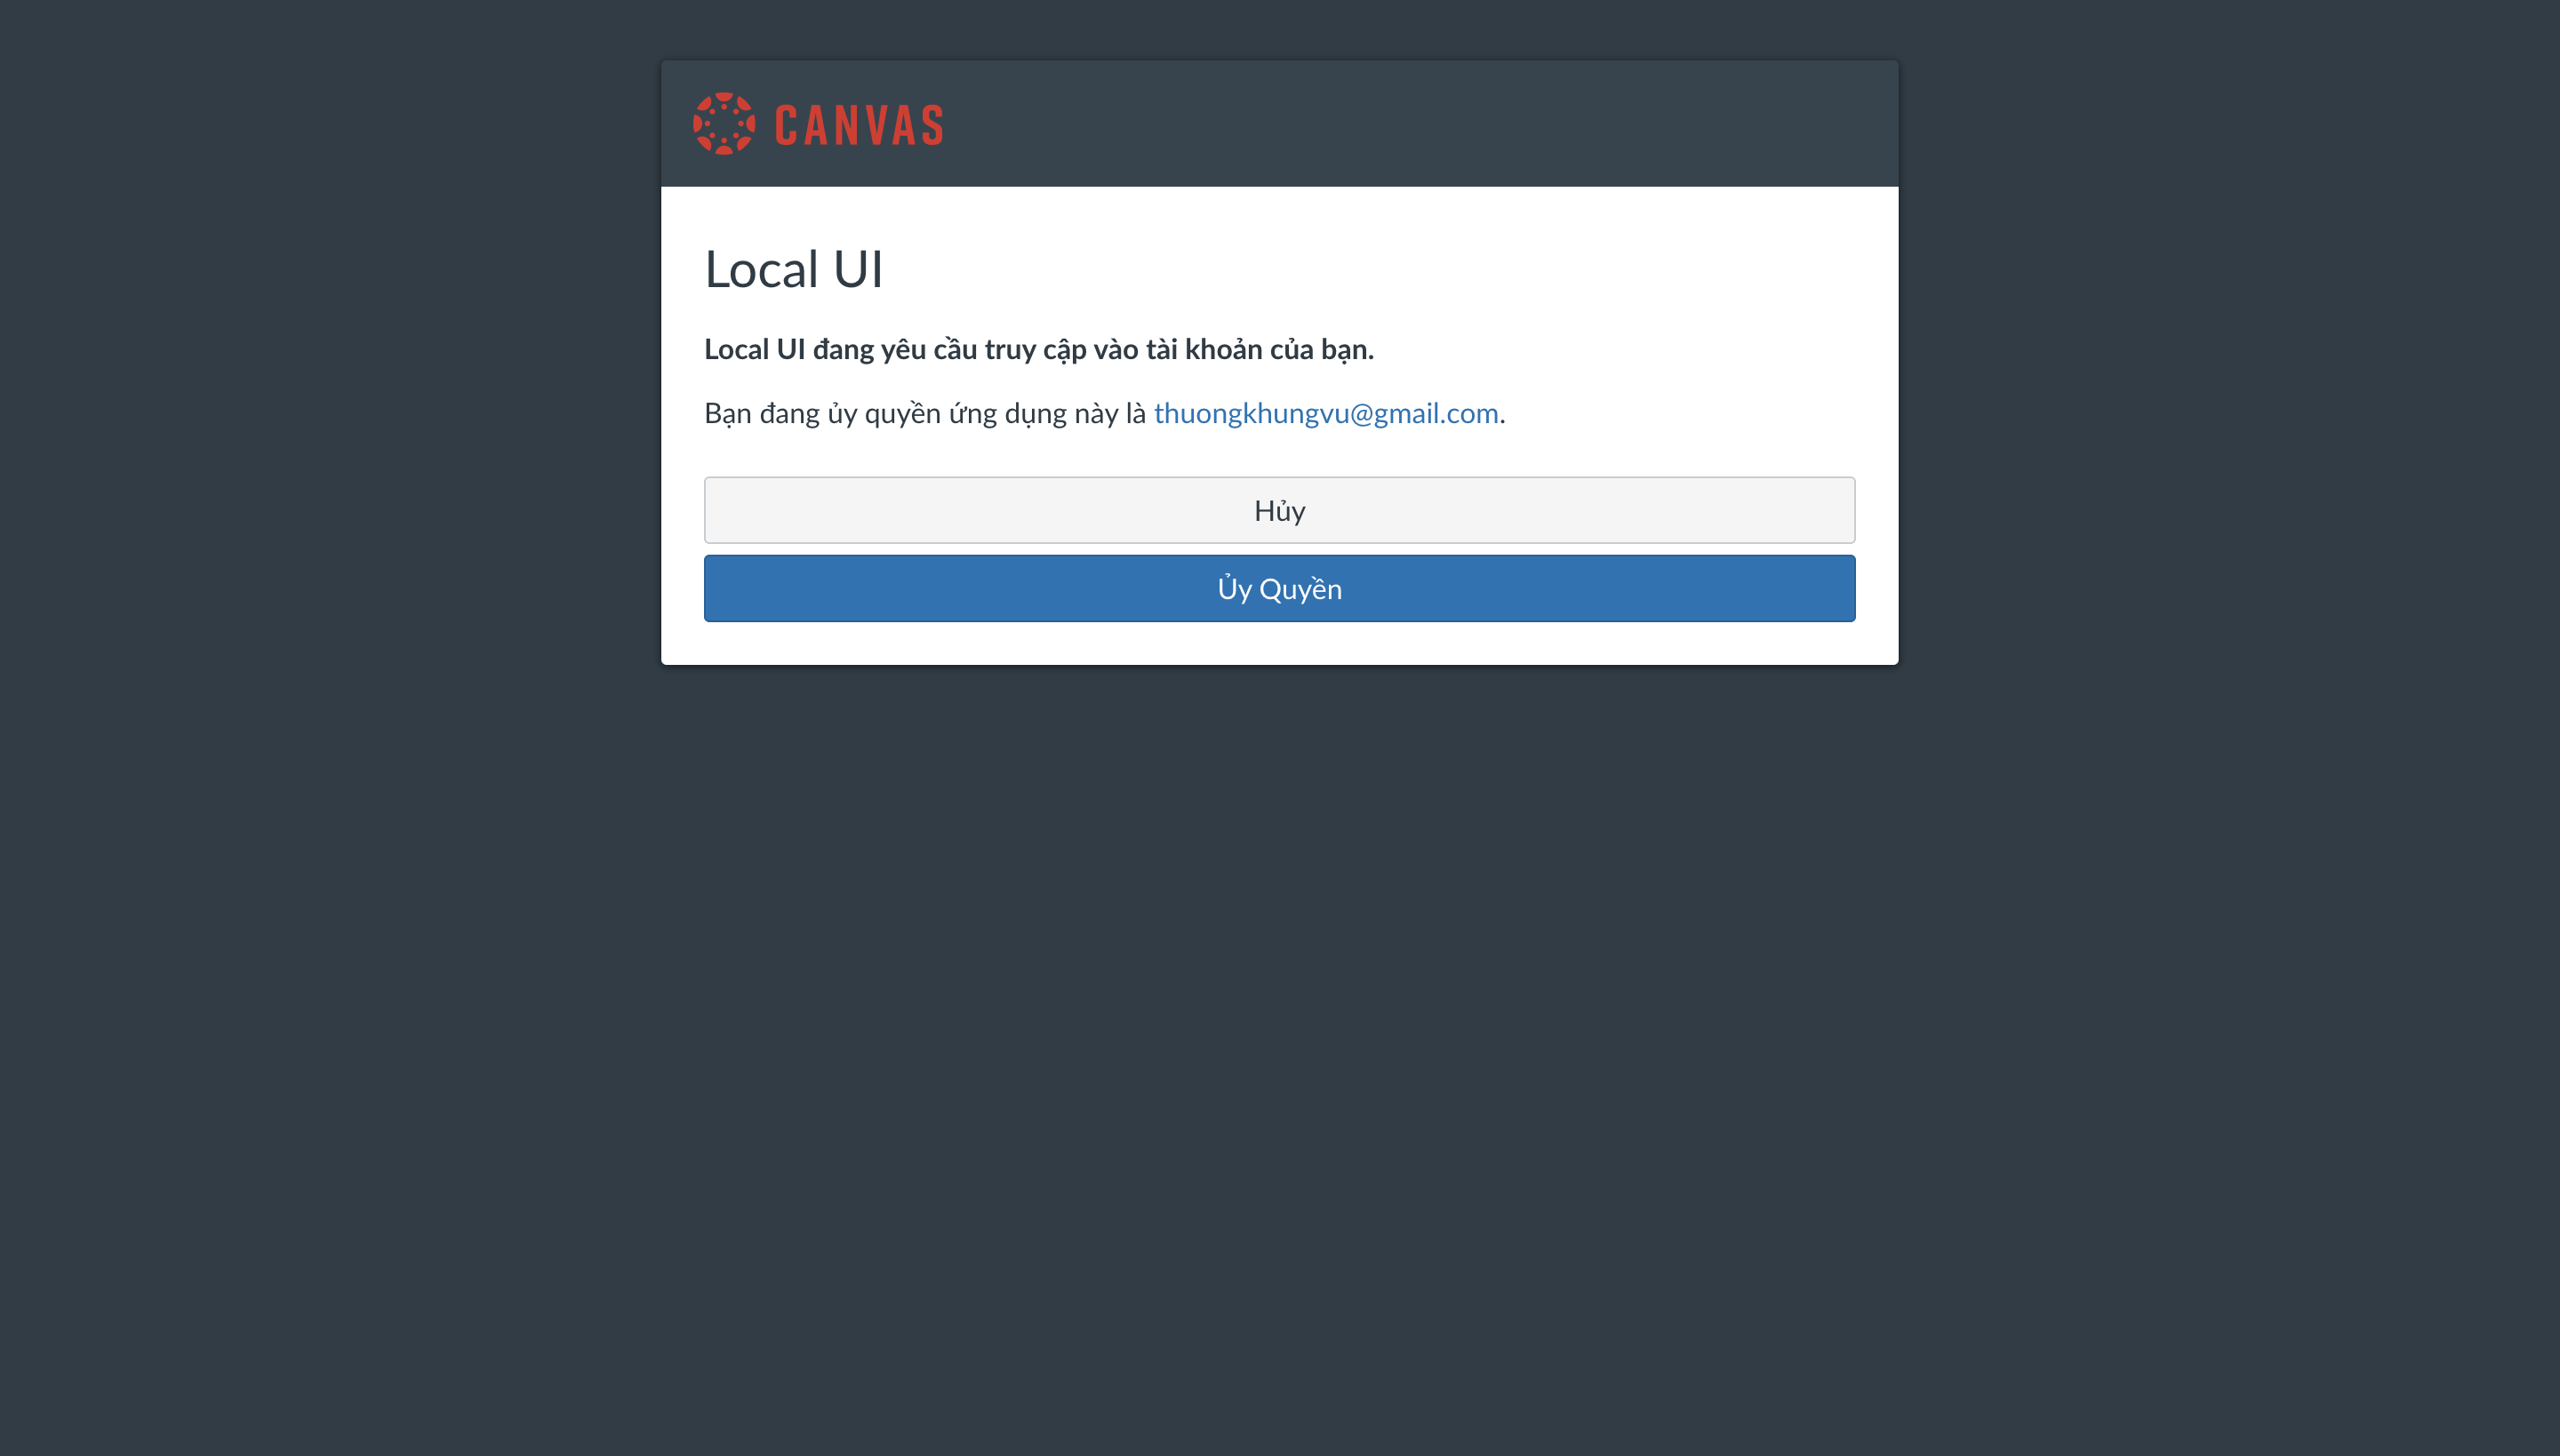
\includegraphics[width=300pt, height=200pt]{dang-nhap-admin}
                    \caption{Màn hình đăng nhập của phần quản trị viên}
                    \label{fig:dang-nhap-admin}
                \end{figure}
                \FloatBarrier

                \item Phần trang chủ của phần quản trị viên được thể hiện ở hình \ref{fig:trang-chu-admin}:
                \begin{figure}[hbt!]
                    \centering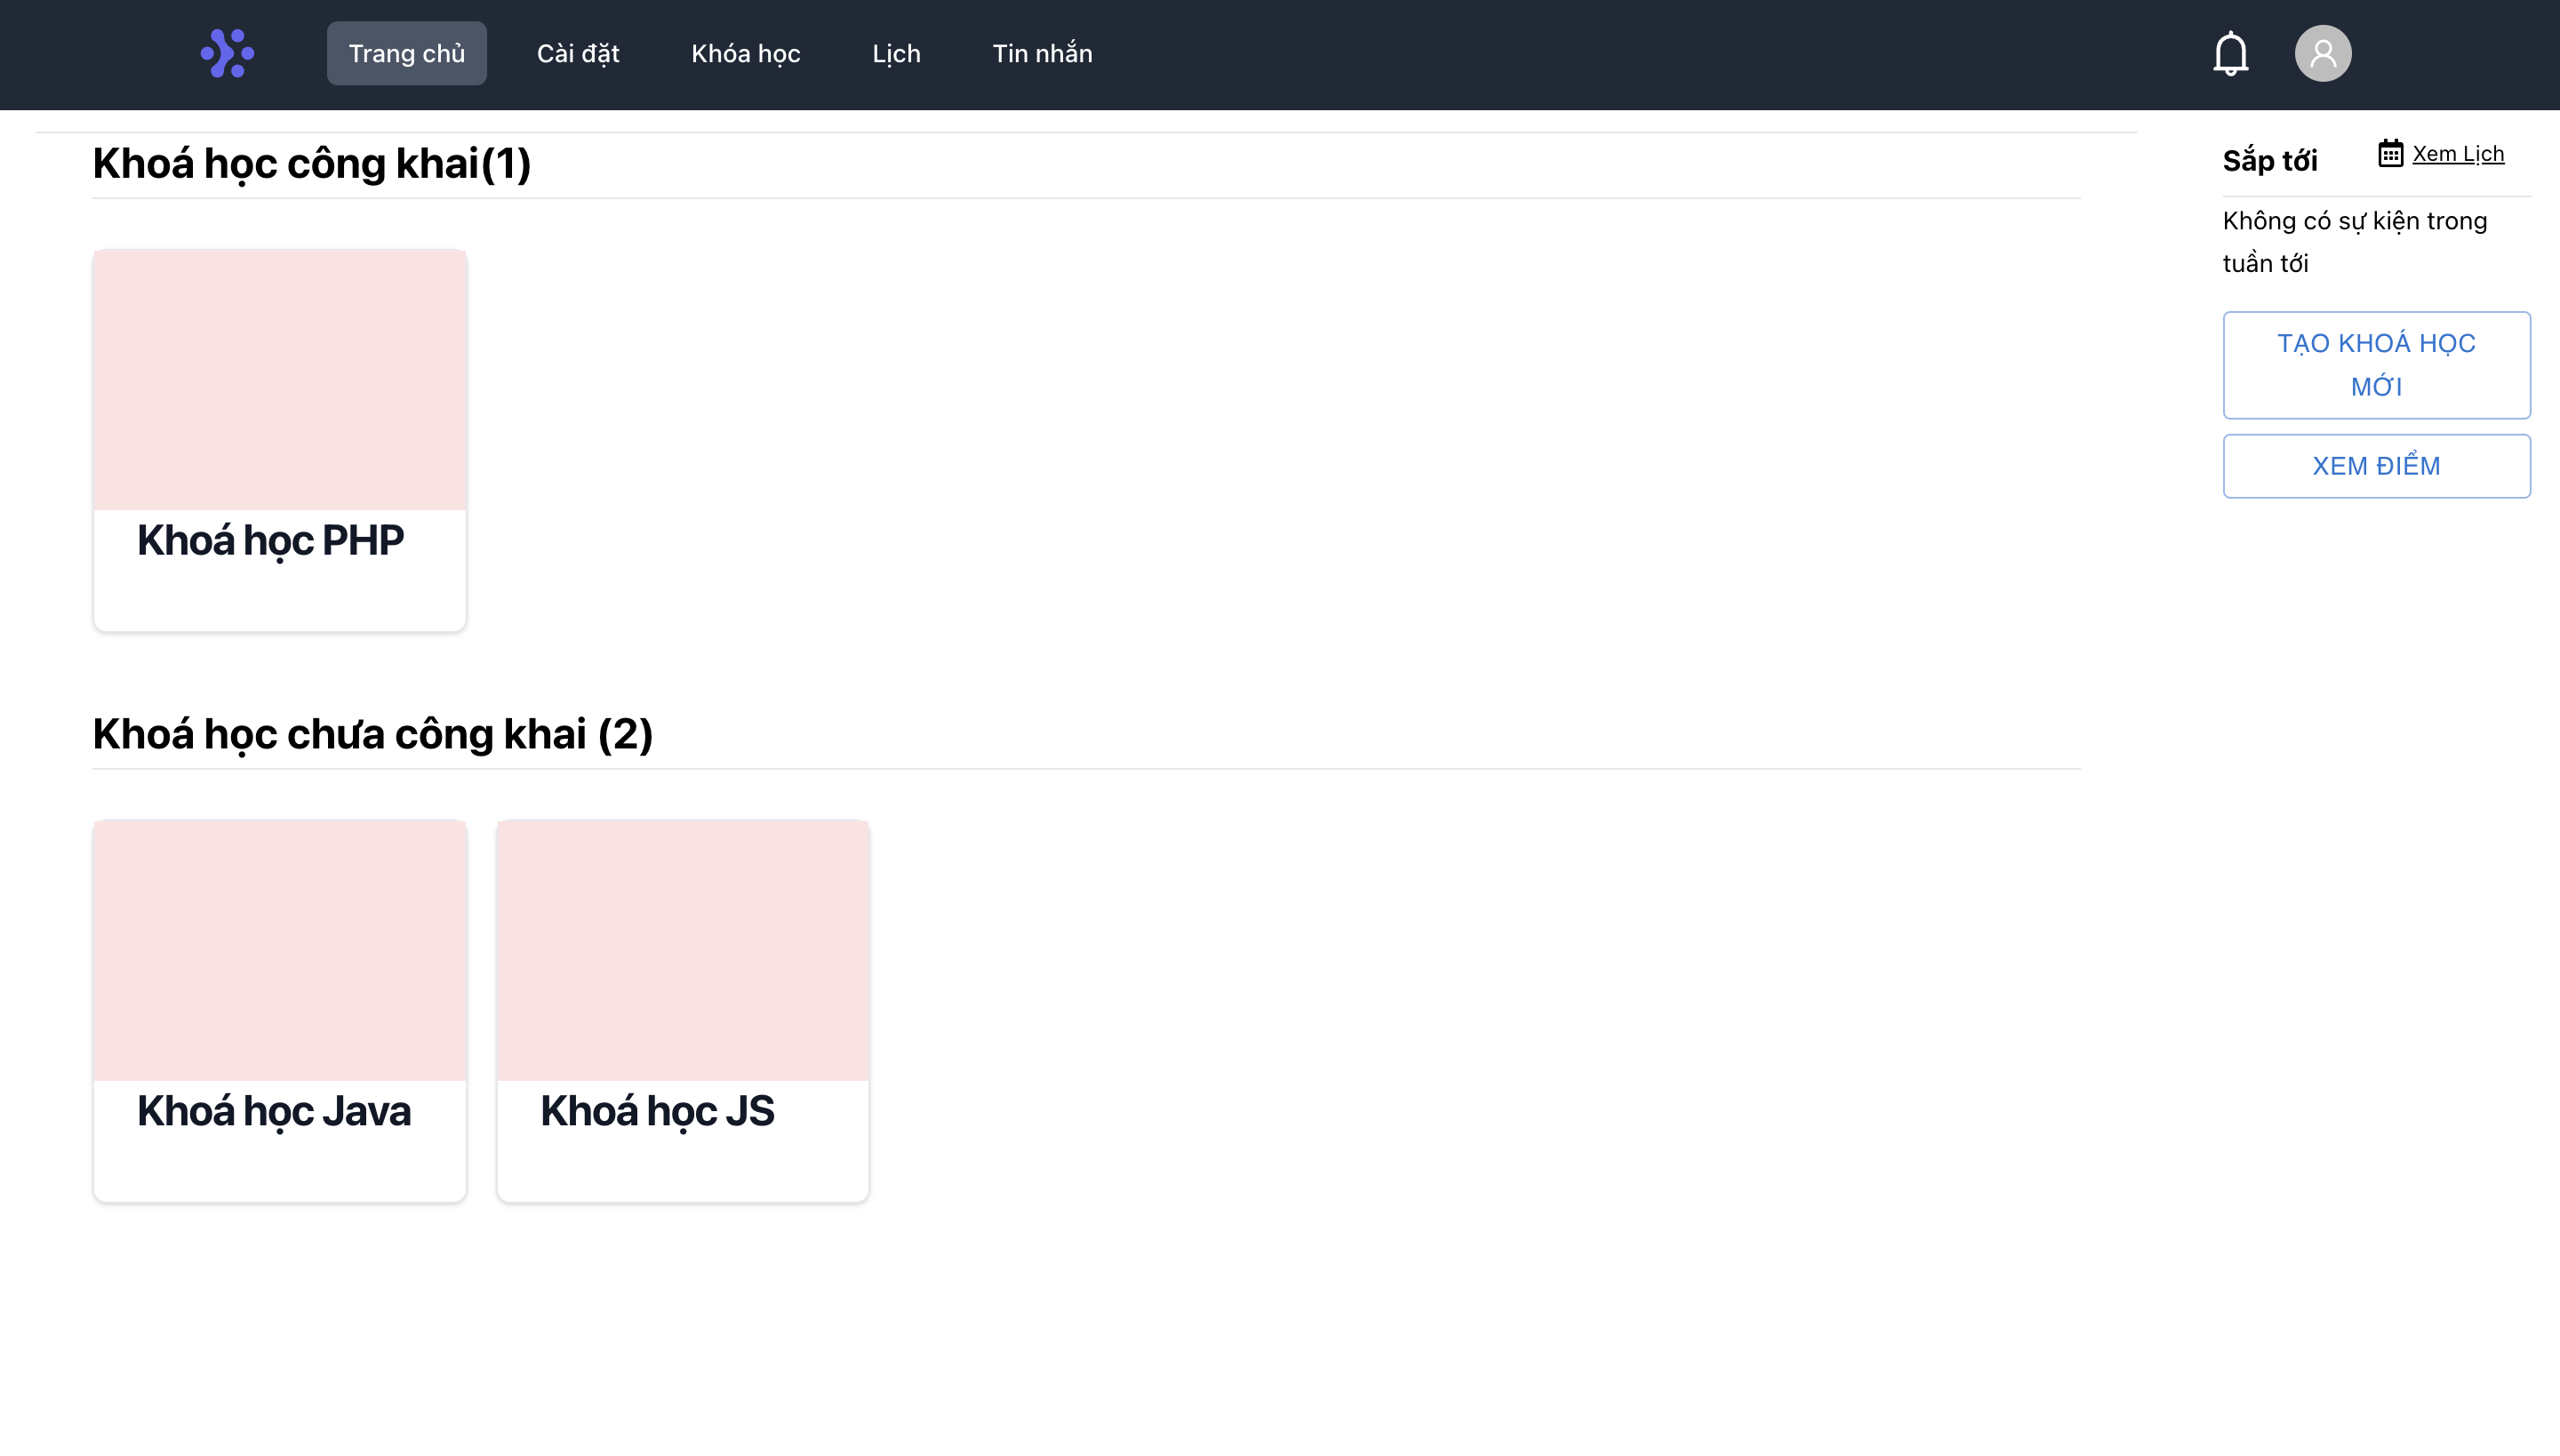
\includegraphics[width=300pt, height=200pt]{trang-chu-admin}
                    \caption{Màn hình trang chủ của phần quản trị viên}
                    \label{fig:trang-chu-admin}
                \end{figure}
                \FloatBarrier

                \item Phần danh sách khoá học của phần quản trị viên được thể hiện ở hình \ref{fig:danh-sach-khoa-hoc}:
                \begin{figure}[hbt!]
                    \centering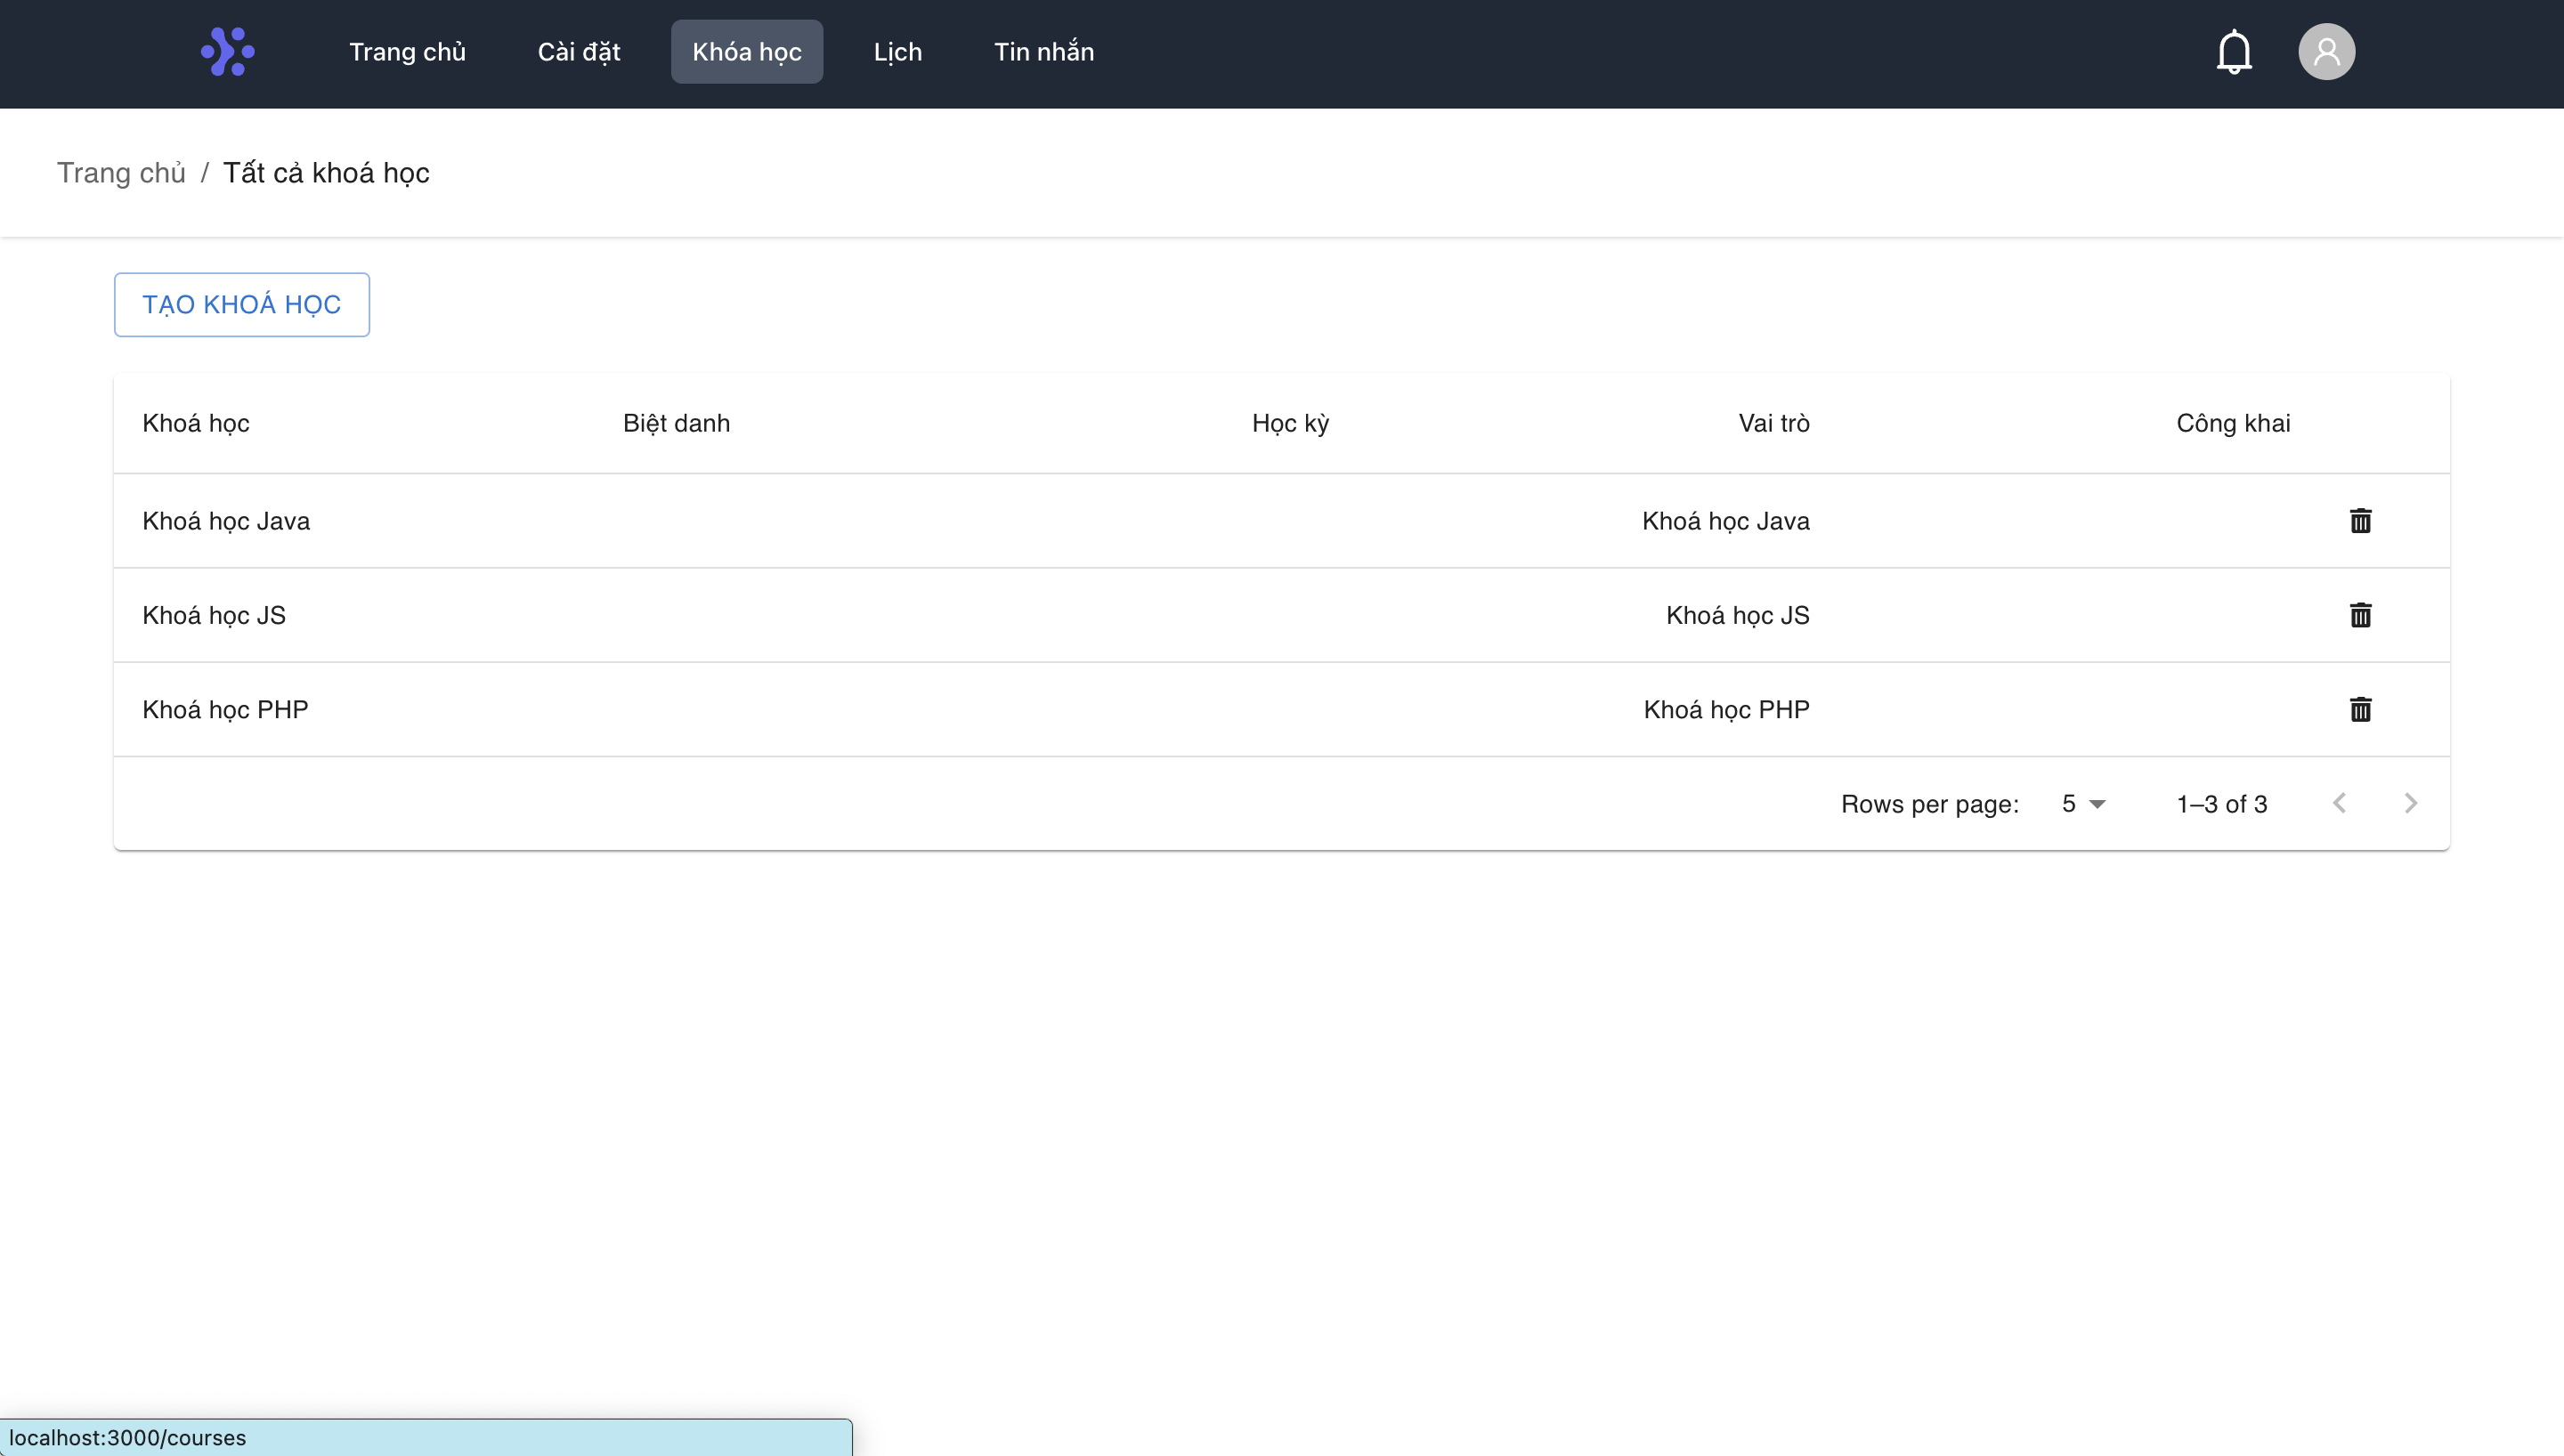
\includegraphics[width=300pt, height=200pt]{danh-sach-khoa-hoc}
                    \caption{Màn hình danh sách khoá học của phần quản trị viên}
                    \label{fig:danh-sach-khoa-hoc}
                \end{figure}
                \FloatBarrier

                \item Phần tạo khoá học của phần quản trị viên được thể hiện ở hình \ref{fig:tao-khoa-hoc}:
                \begin{figure}[hbt!]
                    \centering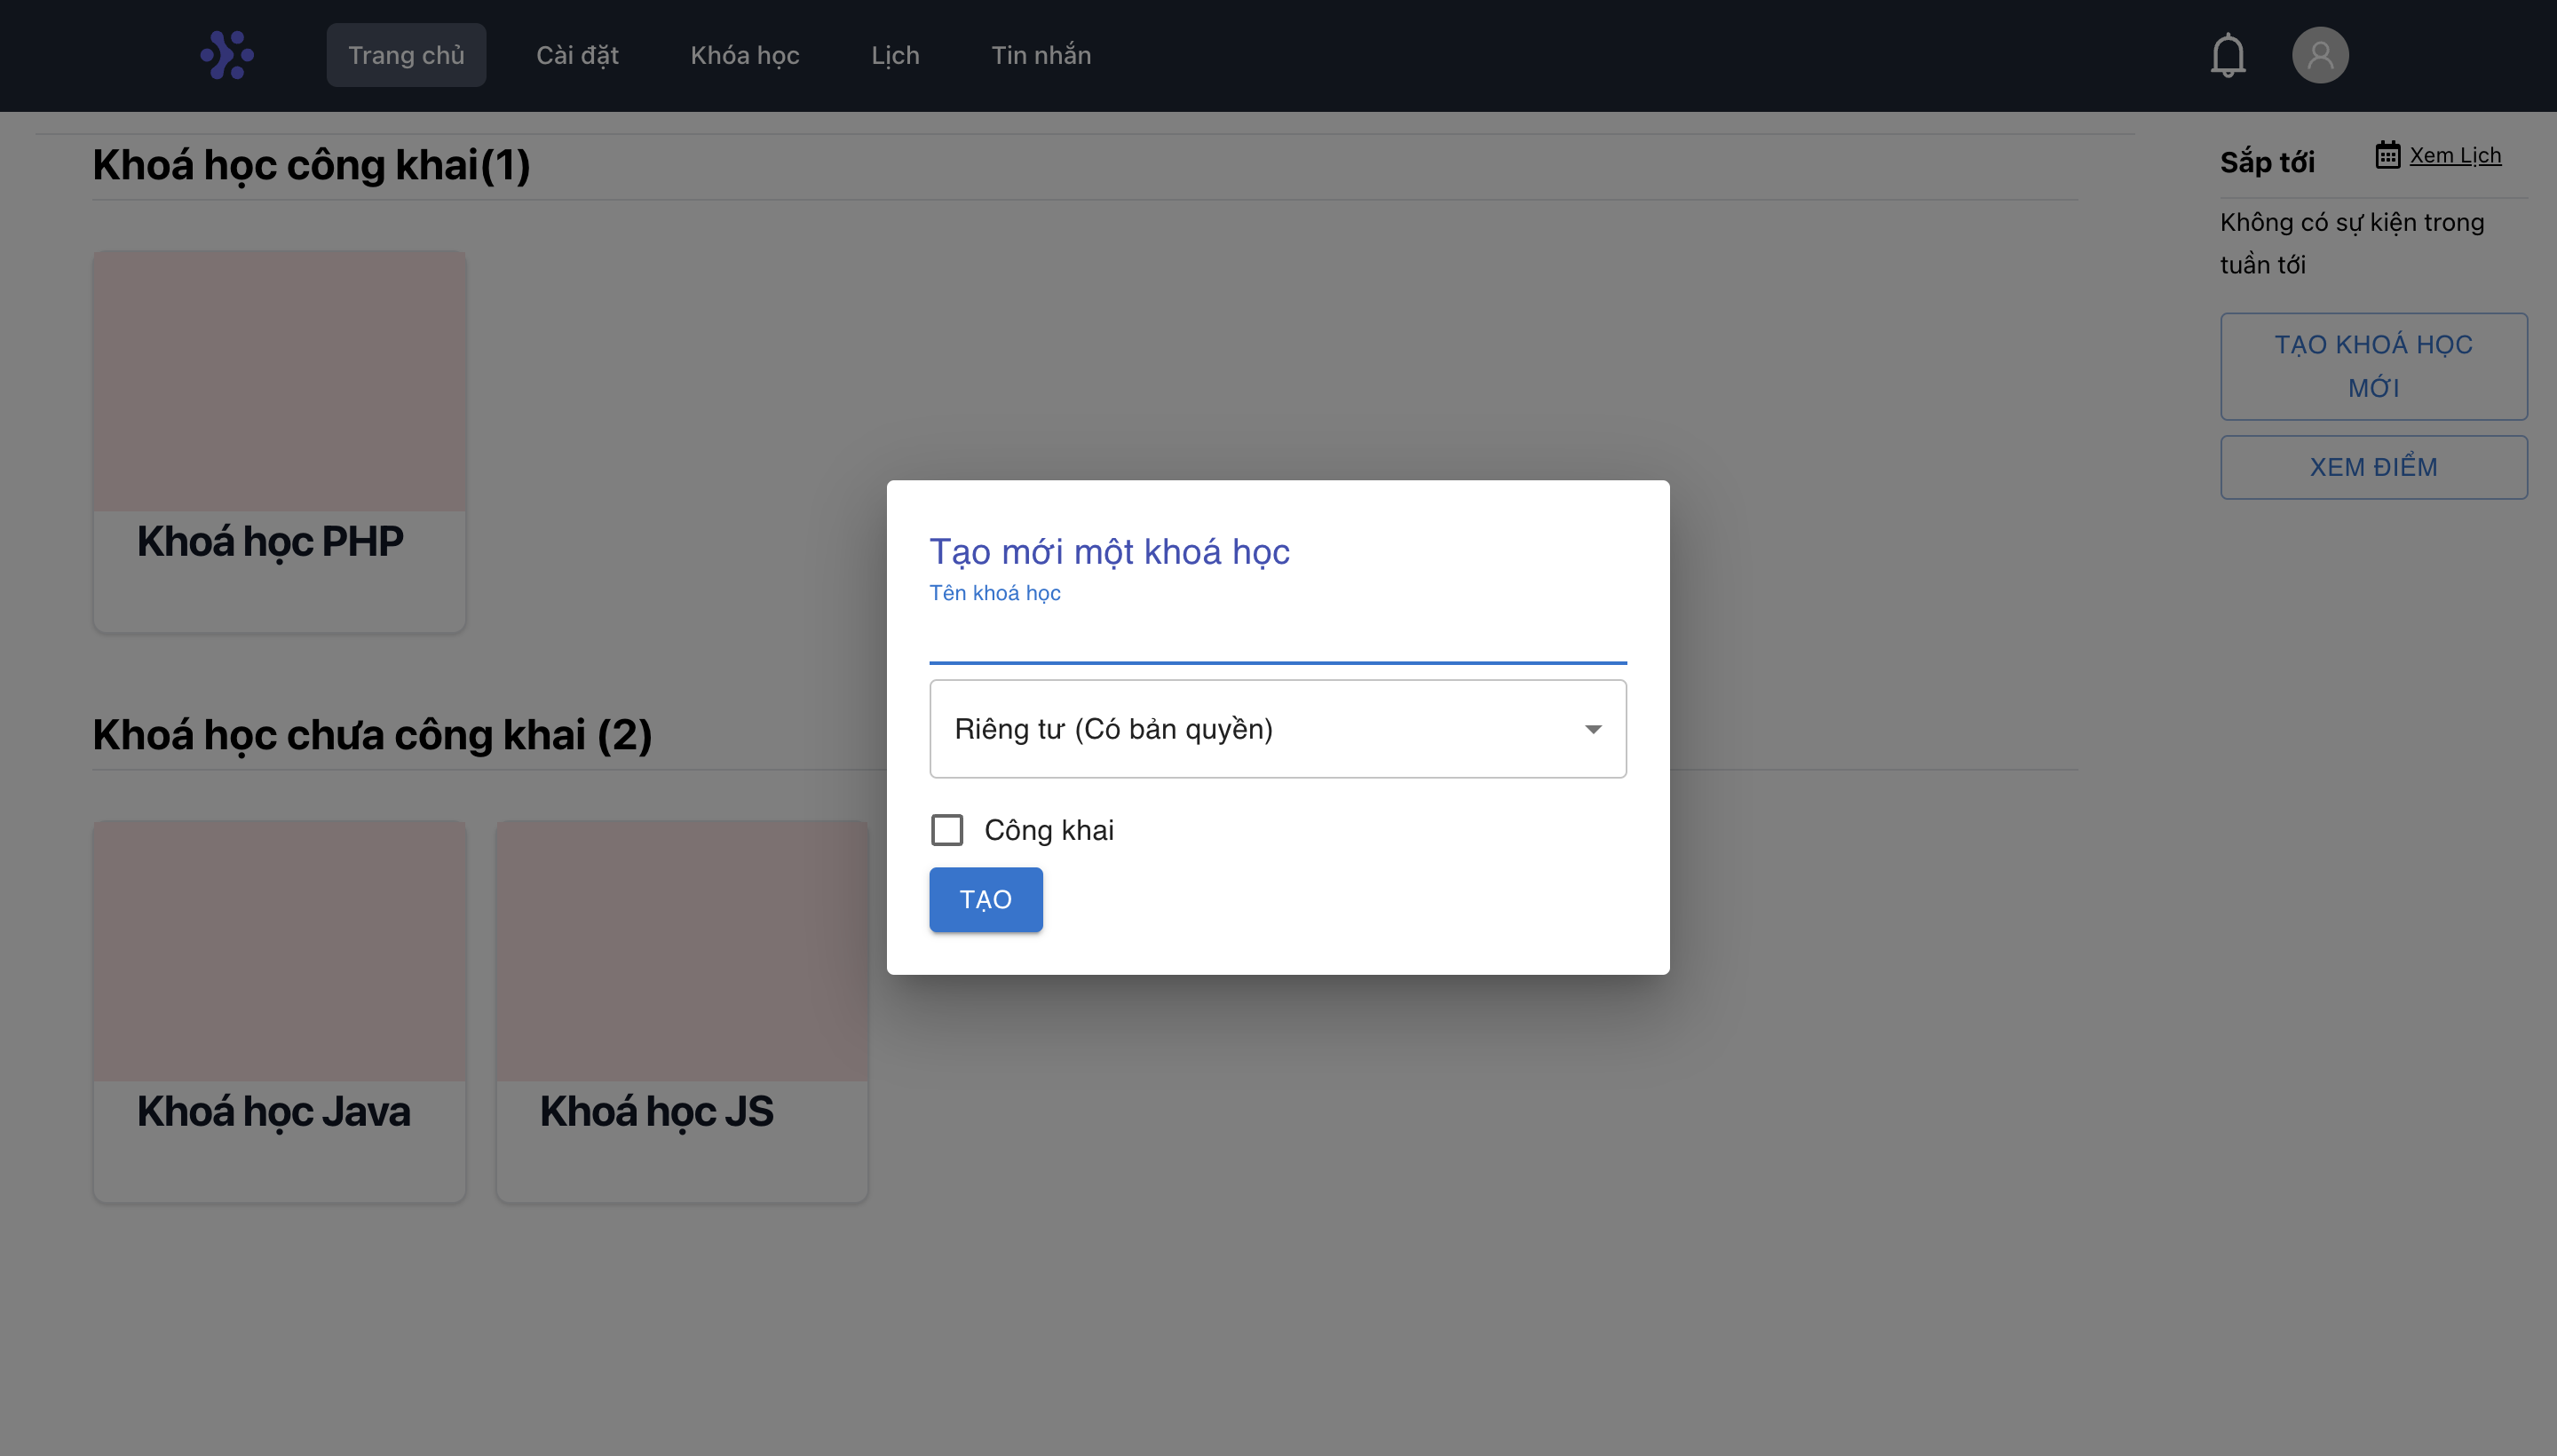
\includegraphics[width=300pt, height=200pt]{tao-khoa-hoc}
                    \caption{Màn hình tạo khoá học của phần quản trị viên}
                    \label{fig:tao-khoa-hoc}
                \end{figure}
                \FloatBarrier


                \item Phần danh sách bài tập và nhóm của phần quản trị viên được thể hiện ở hình \ref{fig:danh-sach-bai-tap}:
                \begin{figure}[hbt!]
                    \centering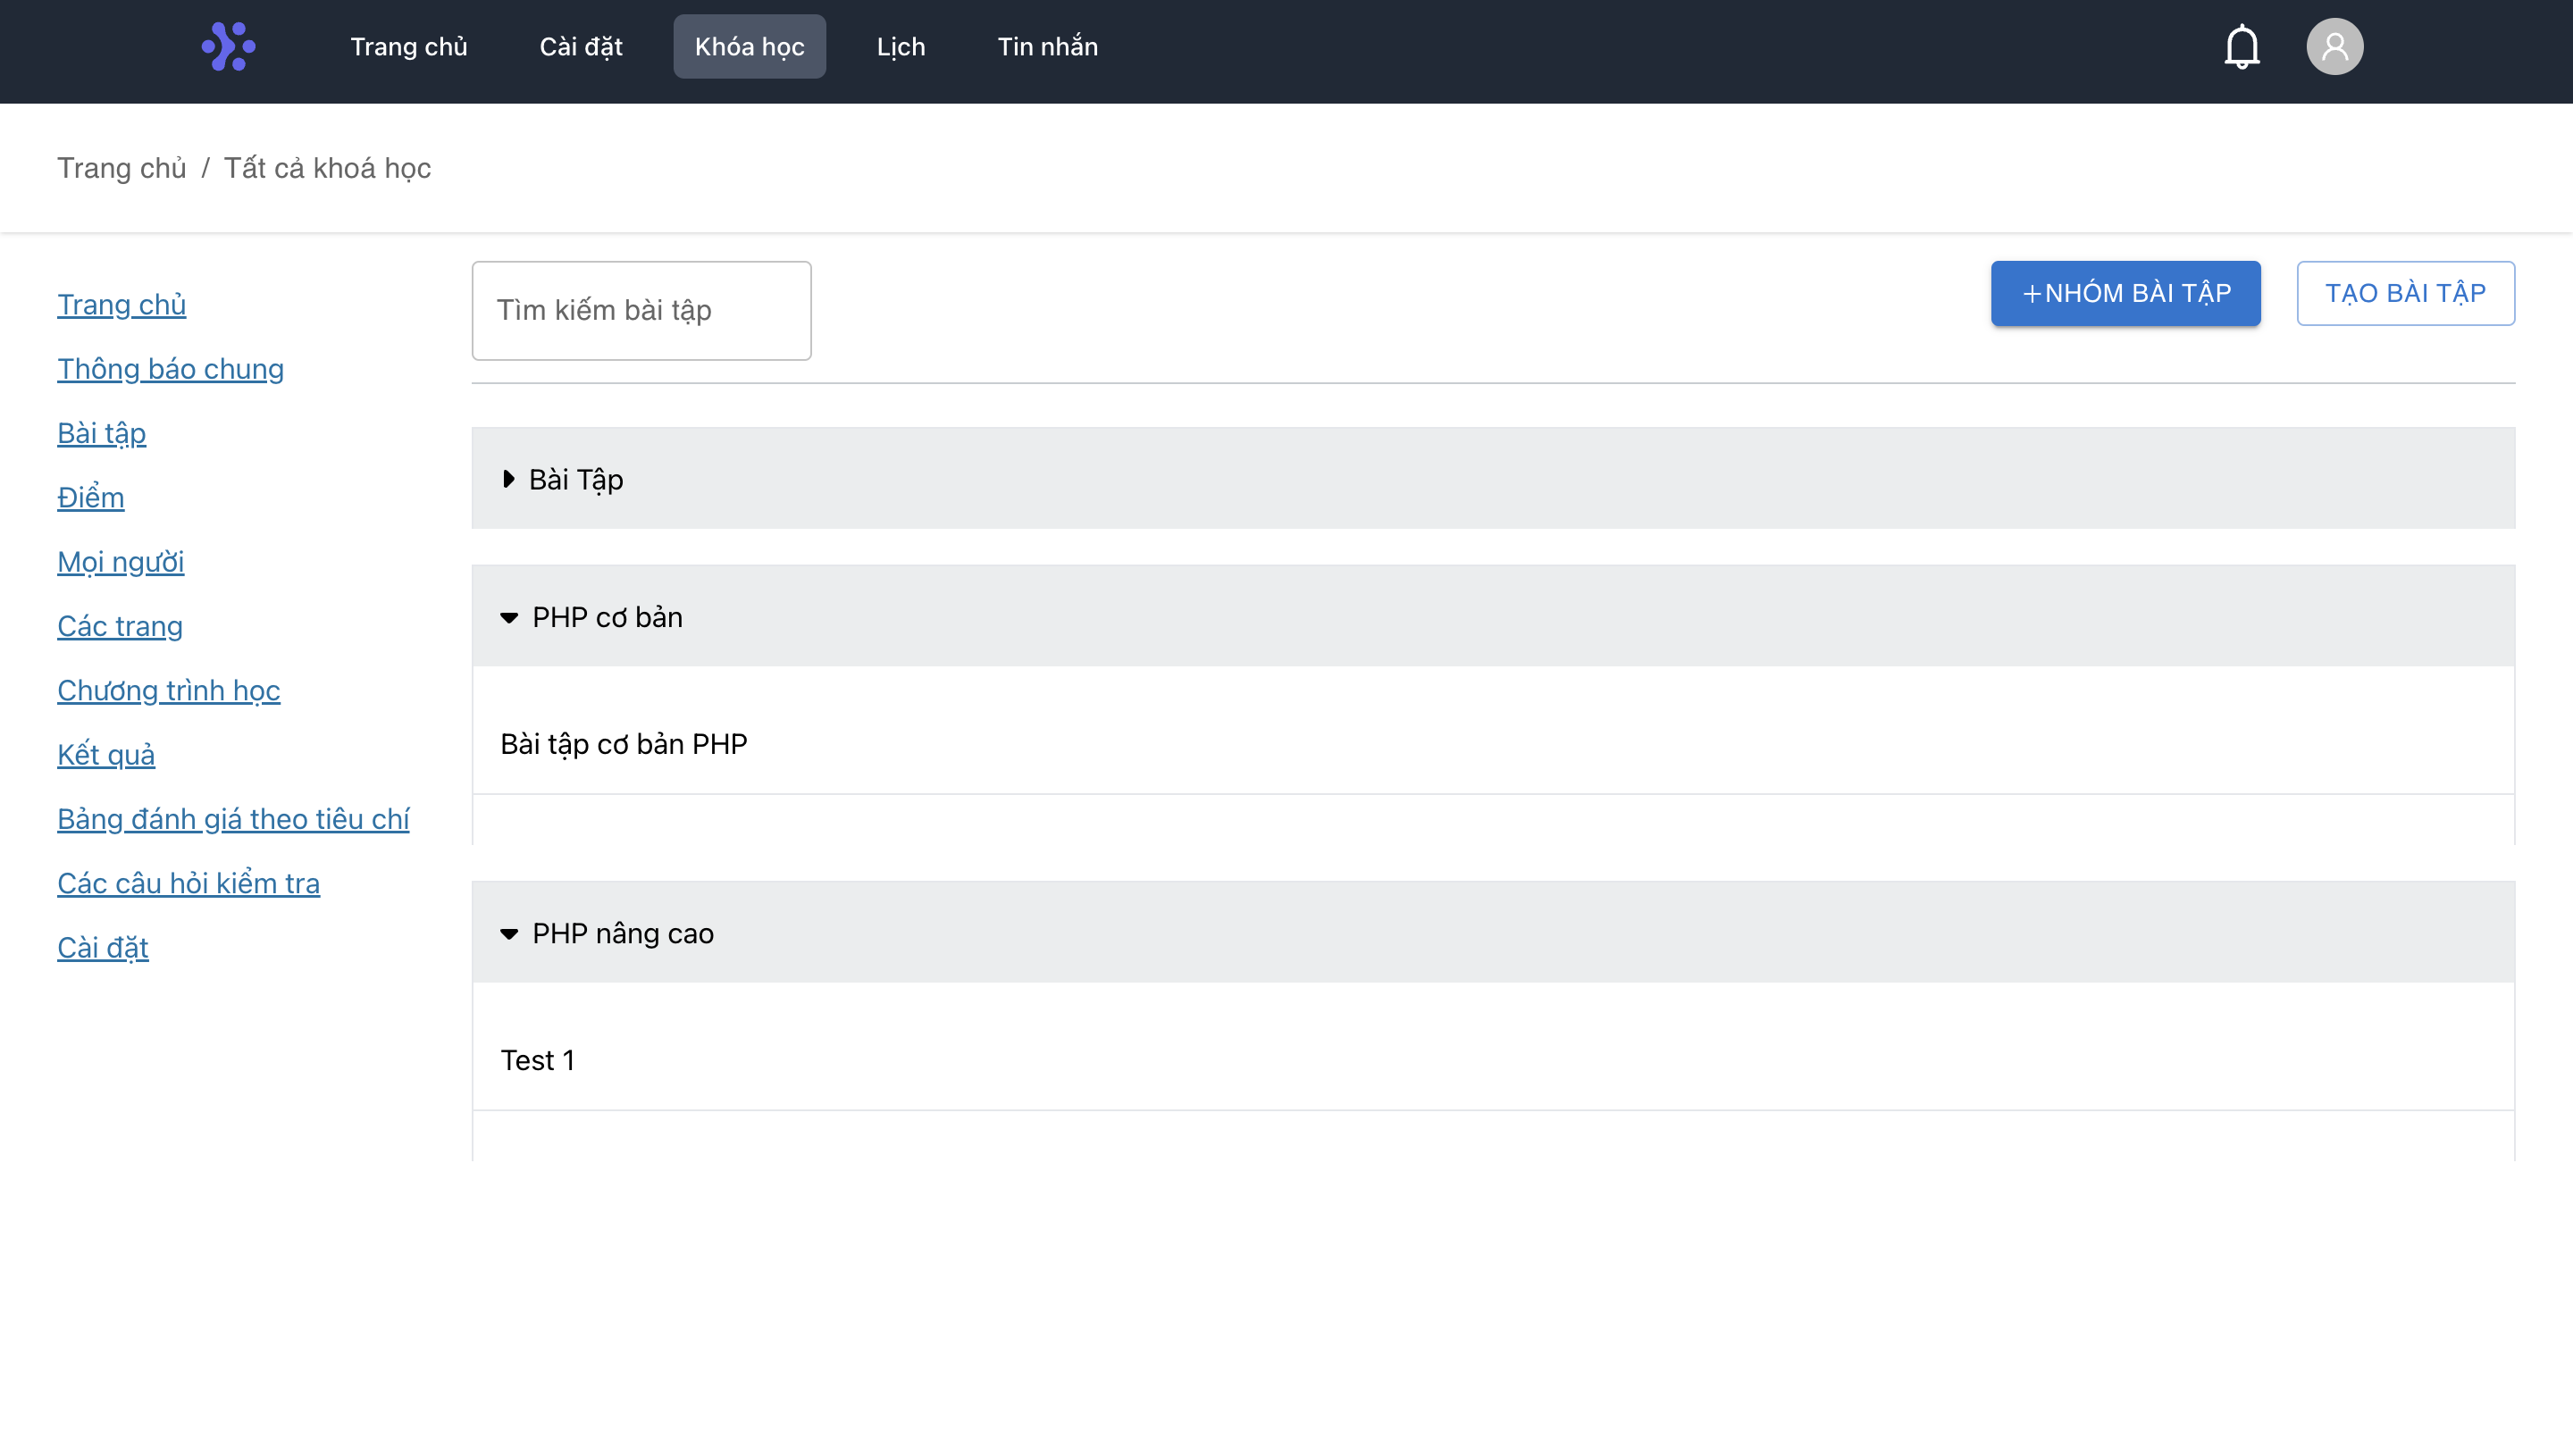
\includegraphics[width=300pt, height=200pt]{danh-sach-bai-tap}
                    \caption{Màn hình danh sách bài tập của phần quản trị viên}
                    \label{fig:danh-sach-bai-tap}
                \end{figure}
                \FloatBarrier

                \item Phần tạo nhóm của phần quản trị viên được thể hiện ở hình \ref{fig:tao-nhom-bai-tap}:
                \begin{figure}[hbt!]
                    \centering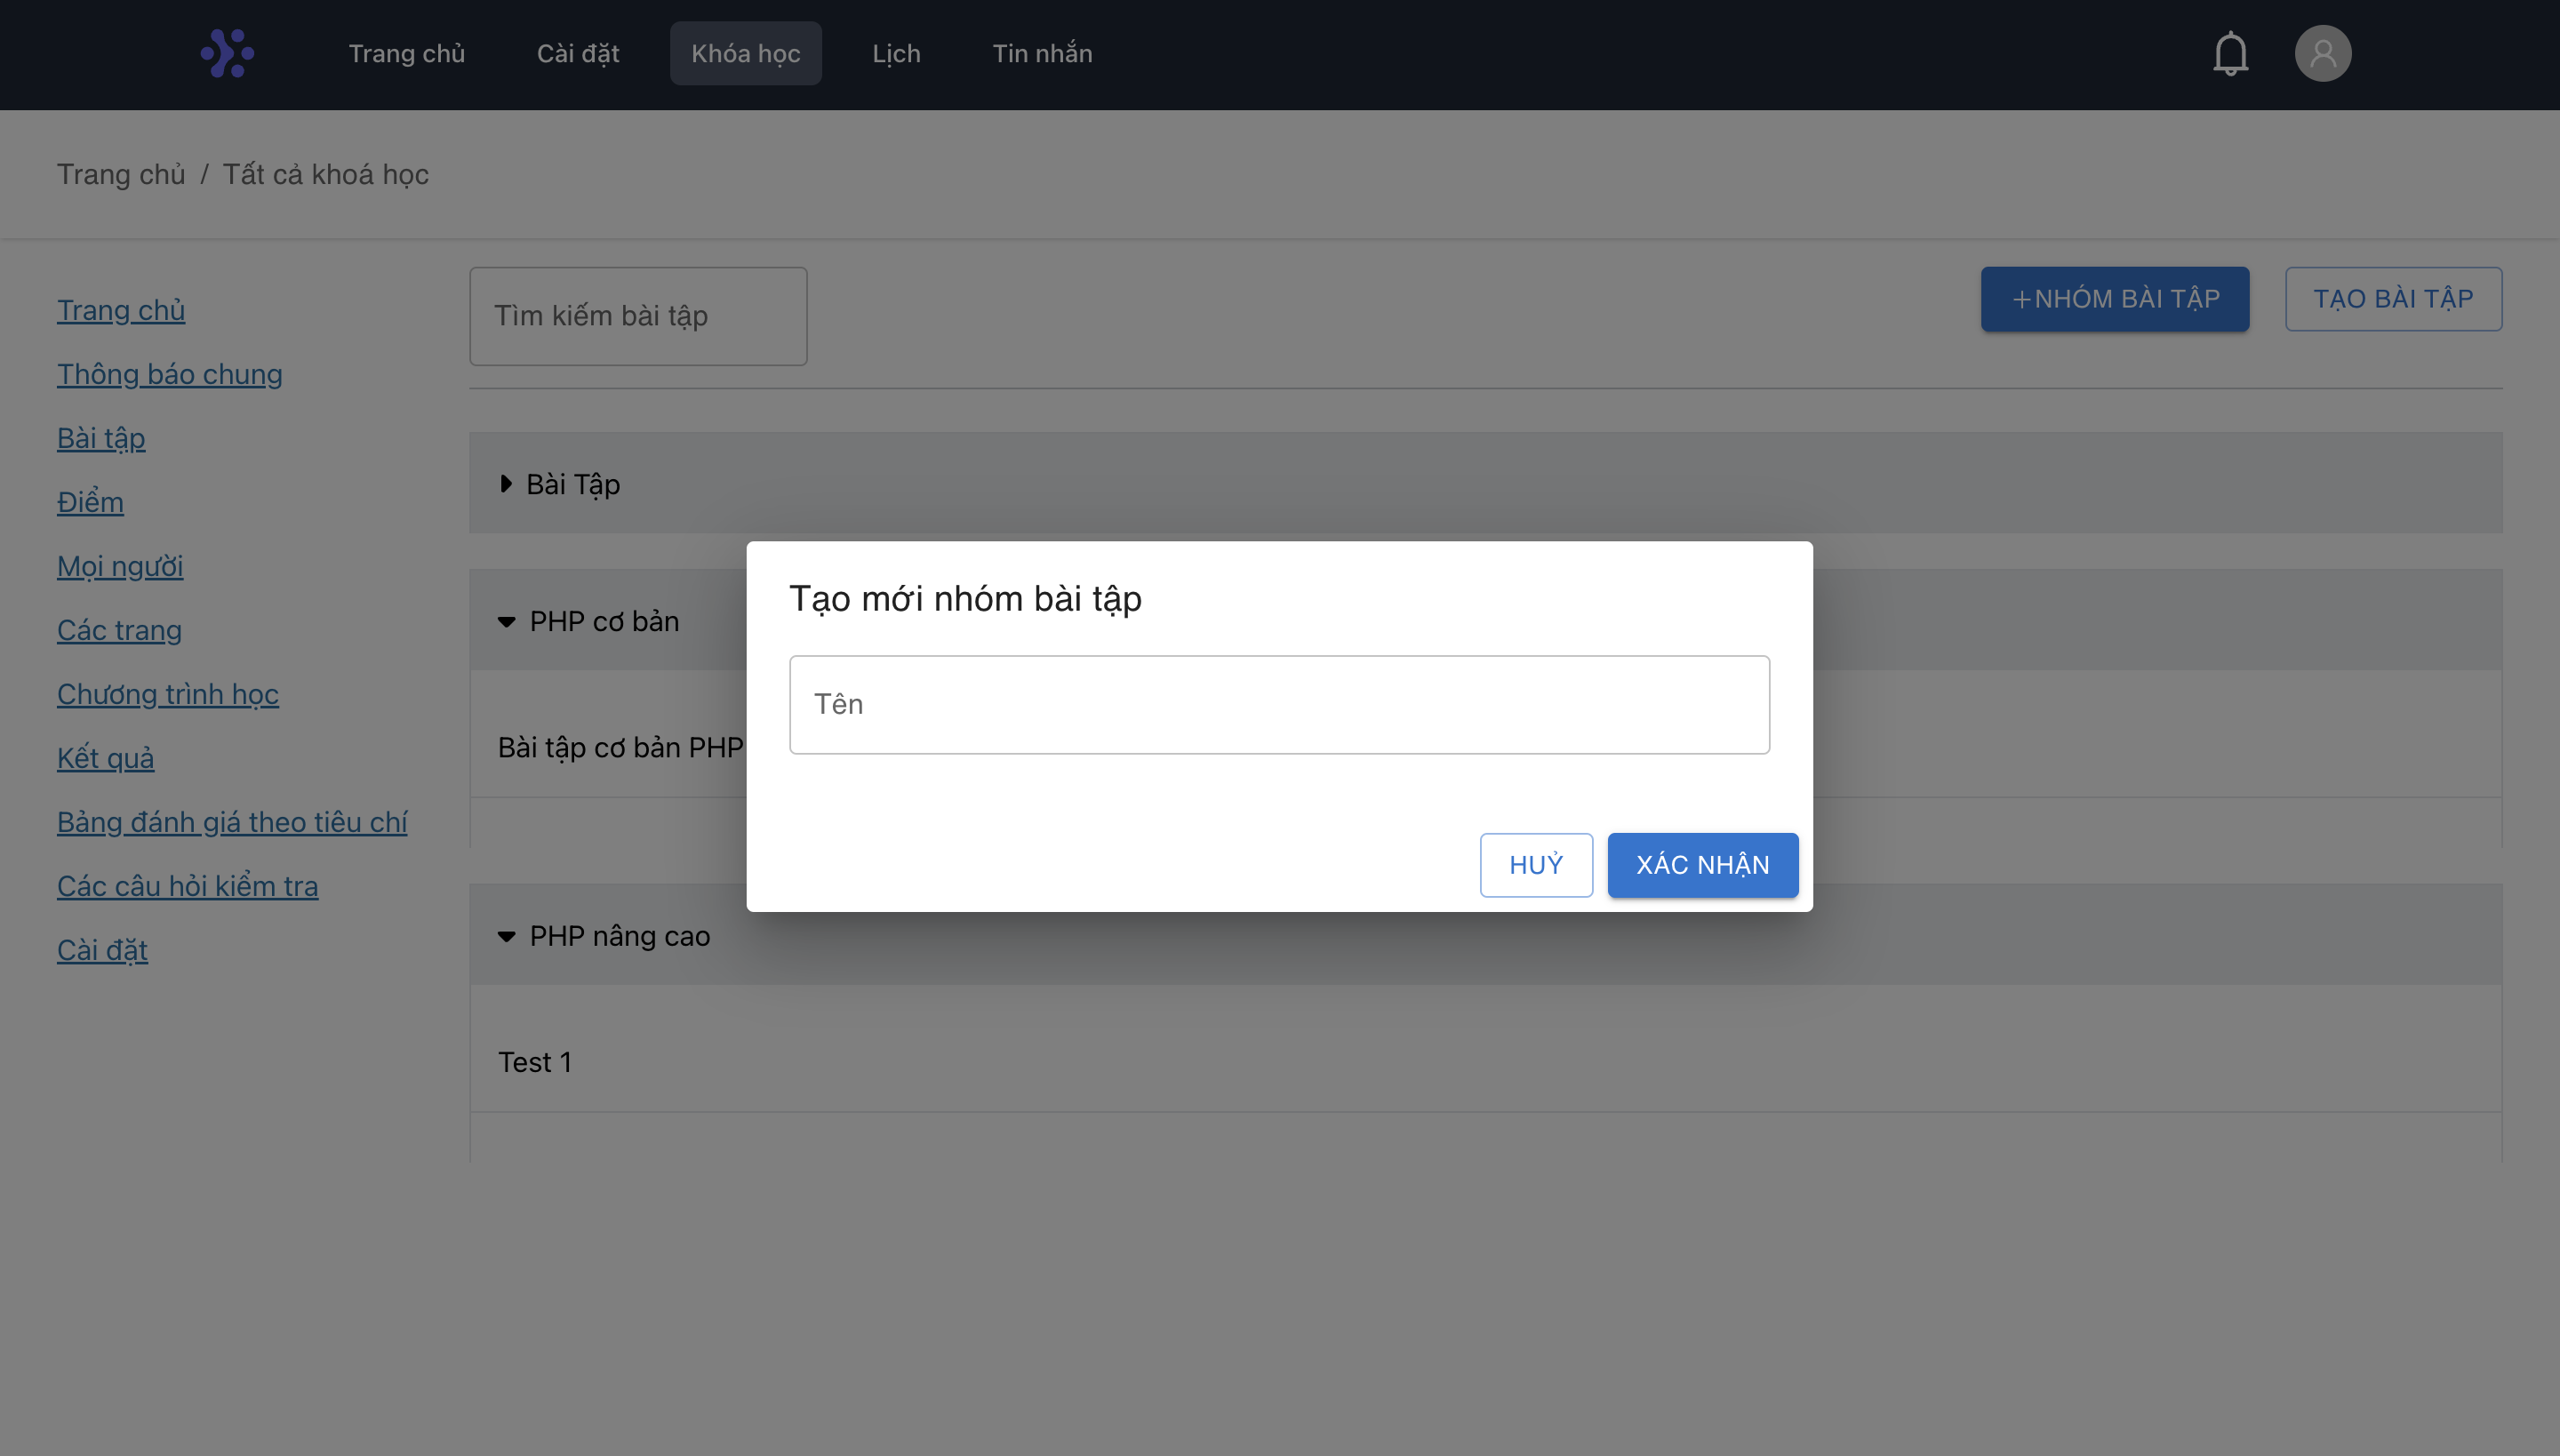
\includegraphics[width=300pt, height=200pt]{tao-nhom-bai-tap}
                    \caption{Màn hình tạo nhóm của phần quản trị viên}
                    \label{fig:tao-nhom-bai-tap}
                \end{figure}
                \FloatBarrier

                \item Phần tạo bài tập của phần quản trị viên được thể hiện ở hình \ref{fig:tao-bai-tap}:
                \begin{figure}[hbt!]
                    \centering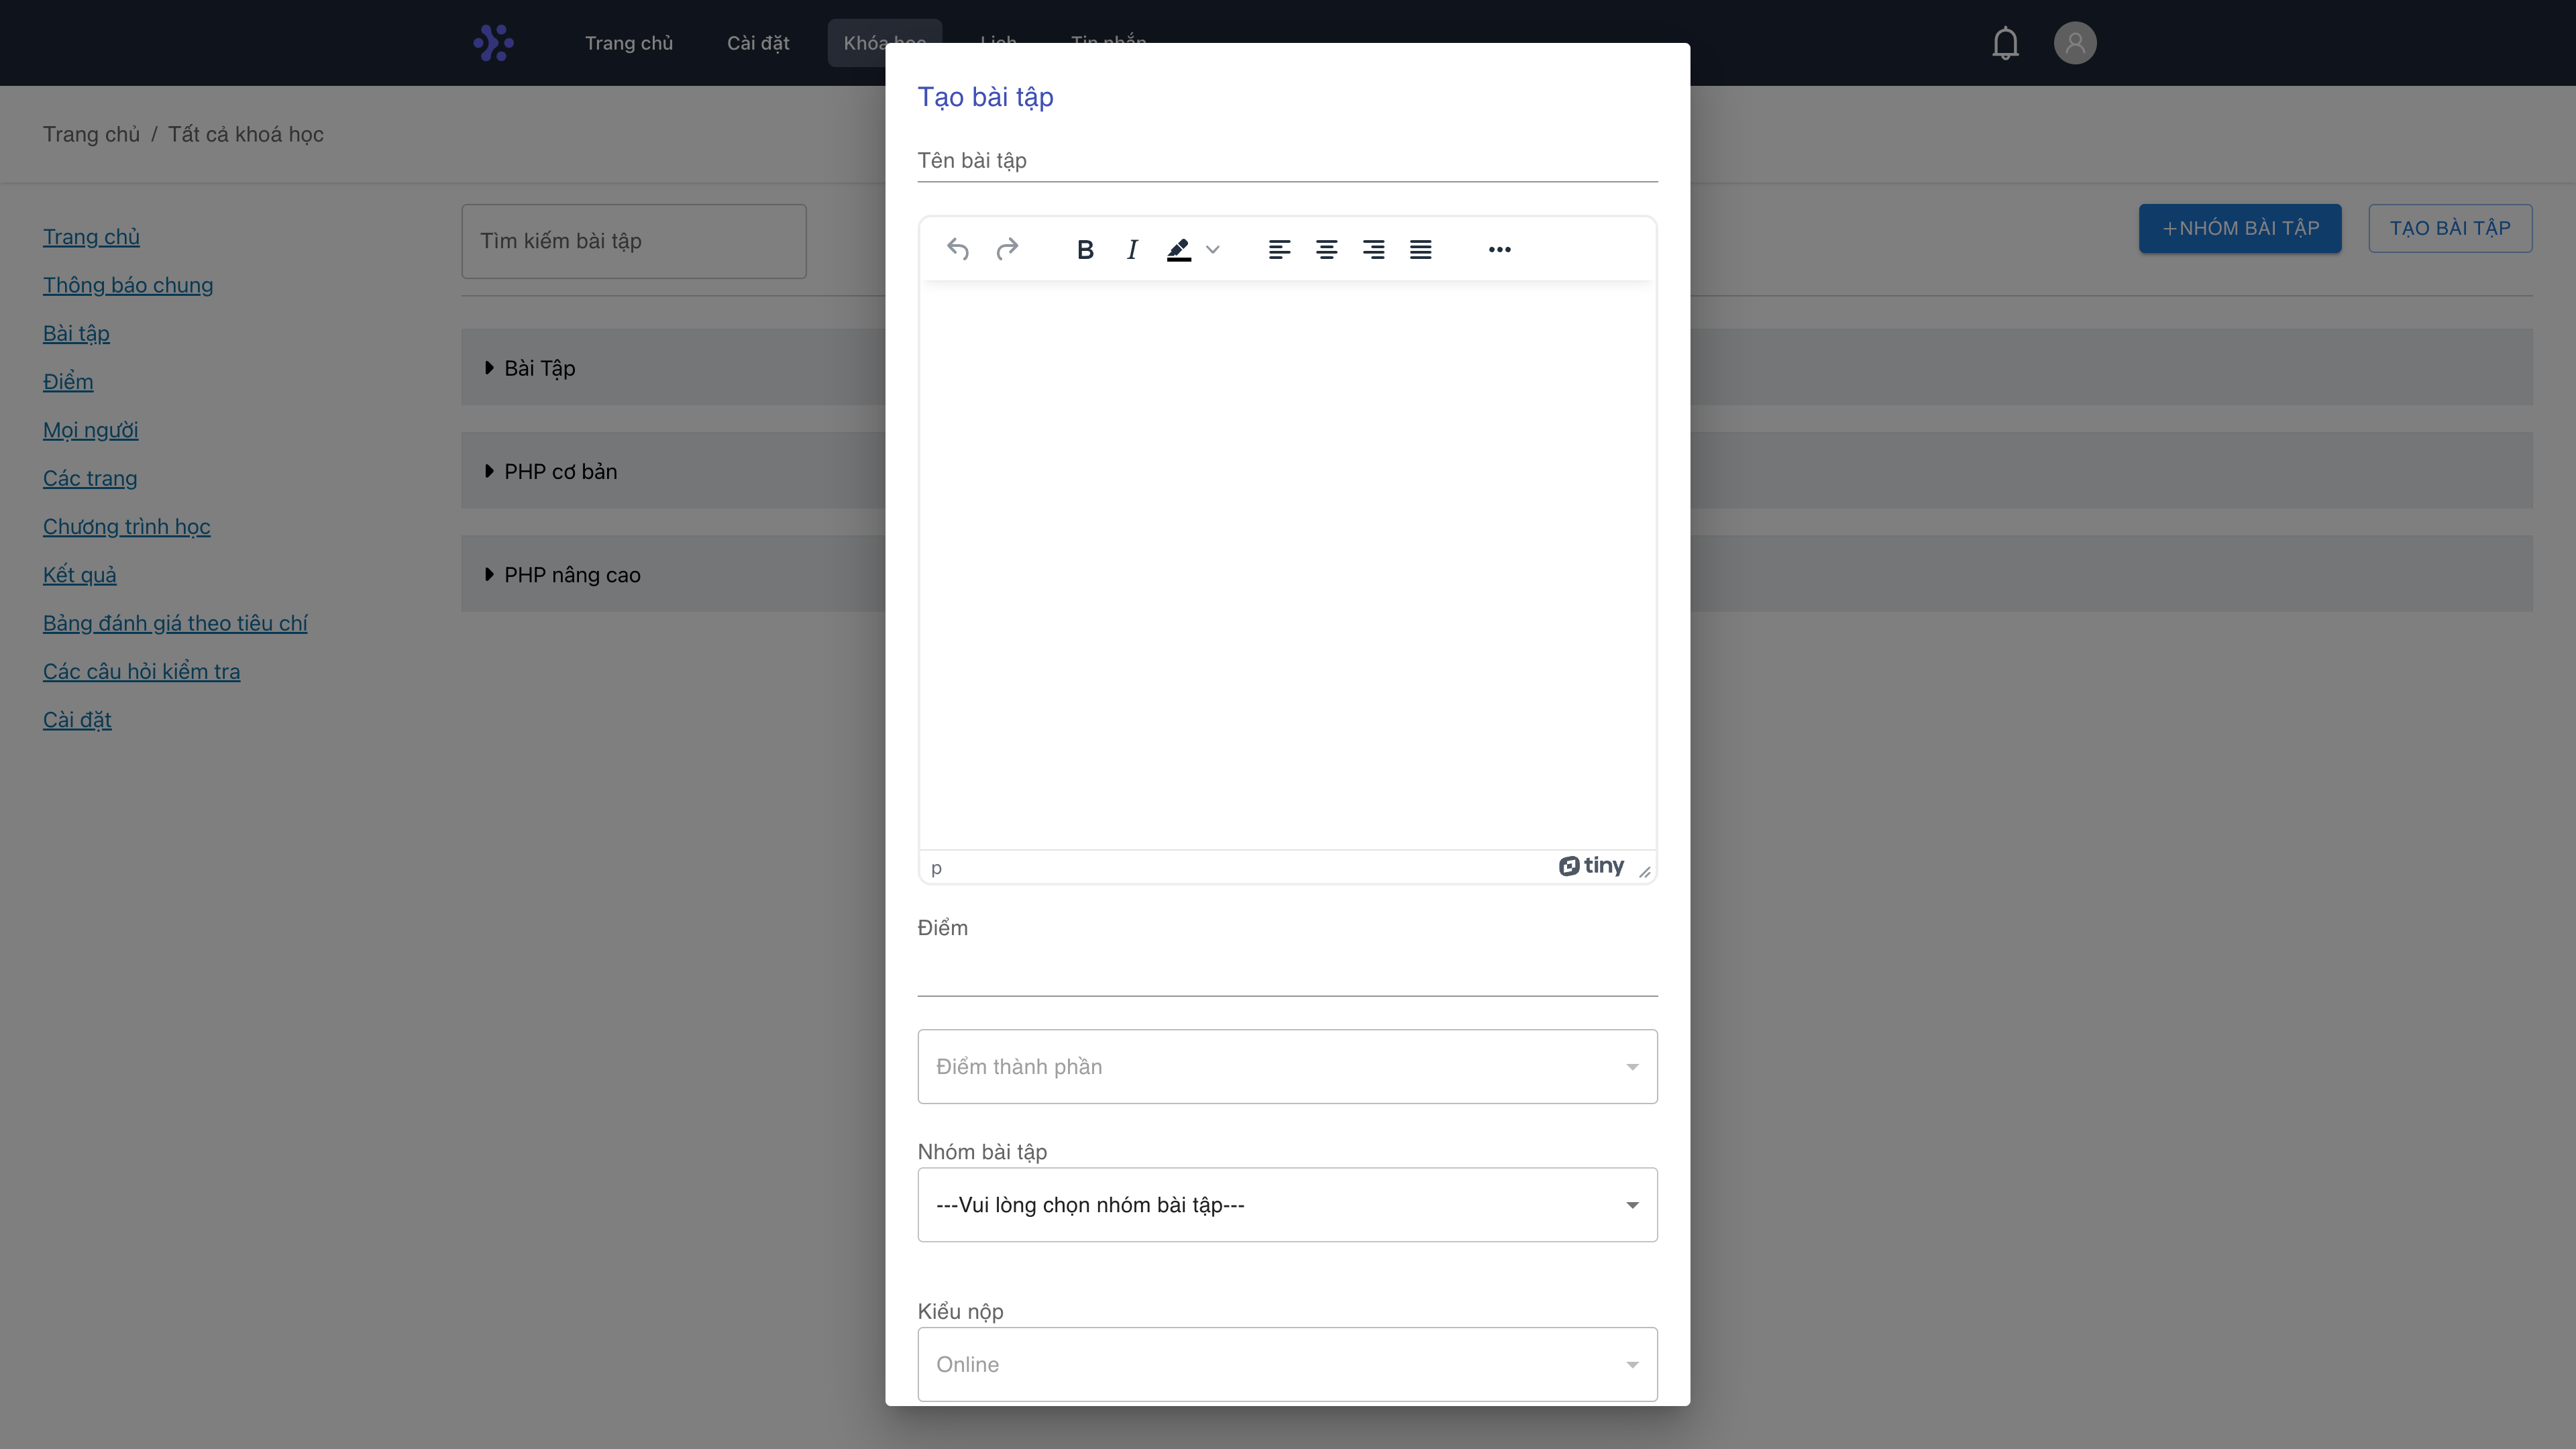
\includegraphics[width=300pt, height=200pt]{tao-bai-tap}
                    \caption{Màn hình tạo bài tập của phần quản trị viên}
                    \label{fig:tao-bai-tap}
                \end{figure}
                \FloatBarrier

                \item Phần chi tiết bài tập của phần quản trị viên được thể hiện ở hình \ref{fig:chi-tiet-bai-tap}:
                \begin{figure}[hbt!]
                    \centering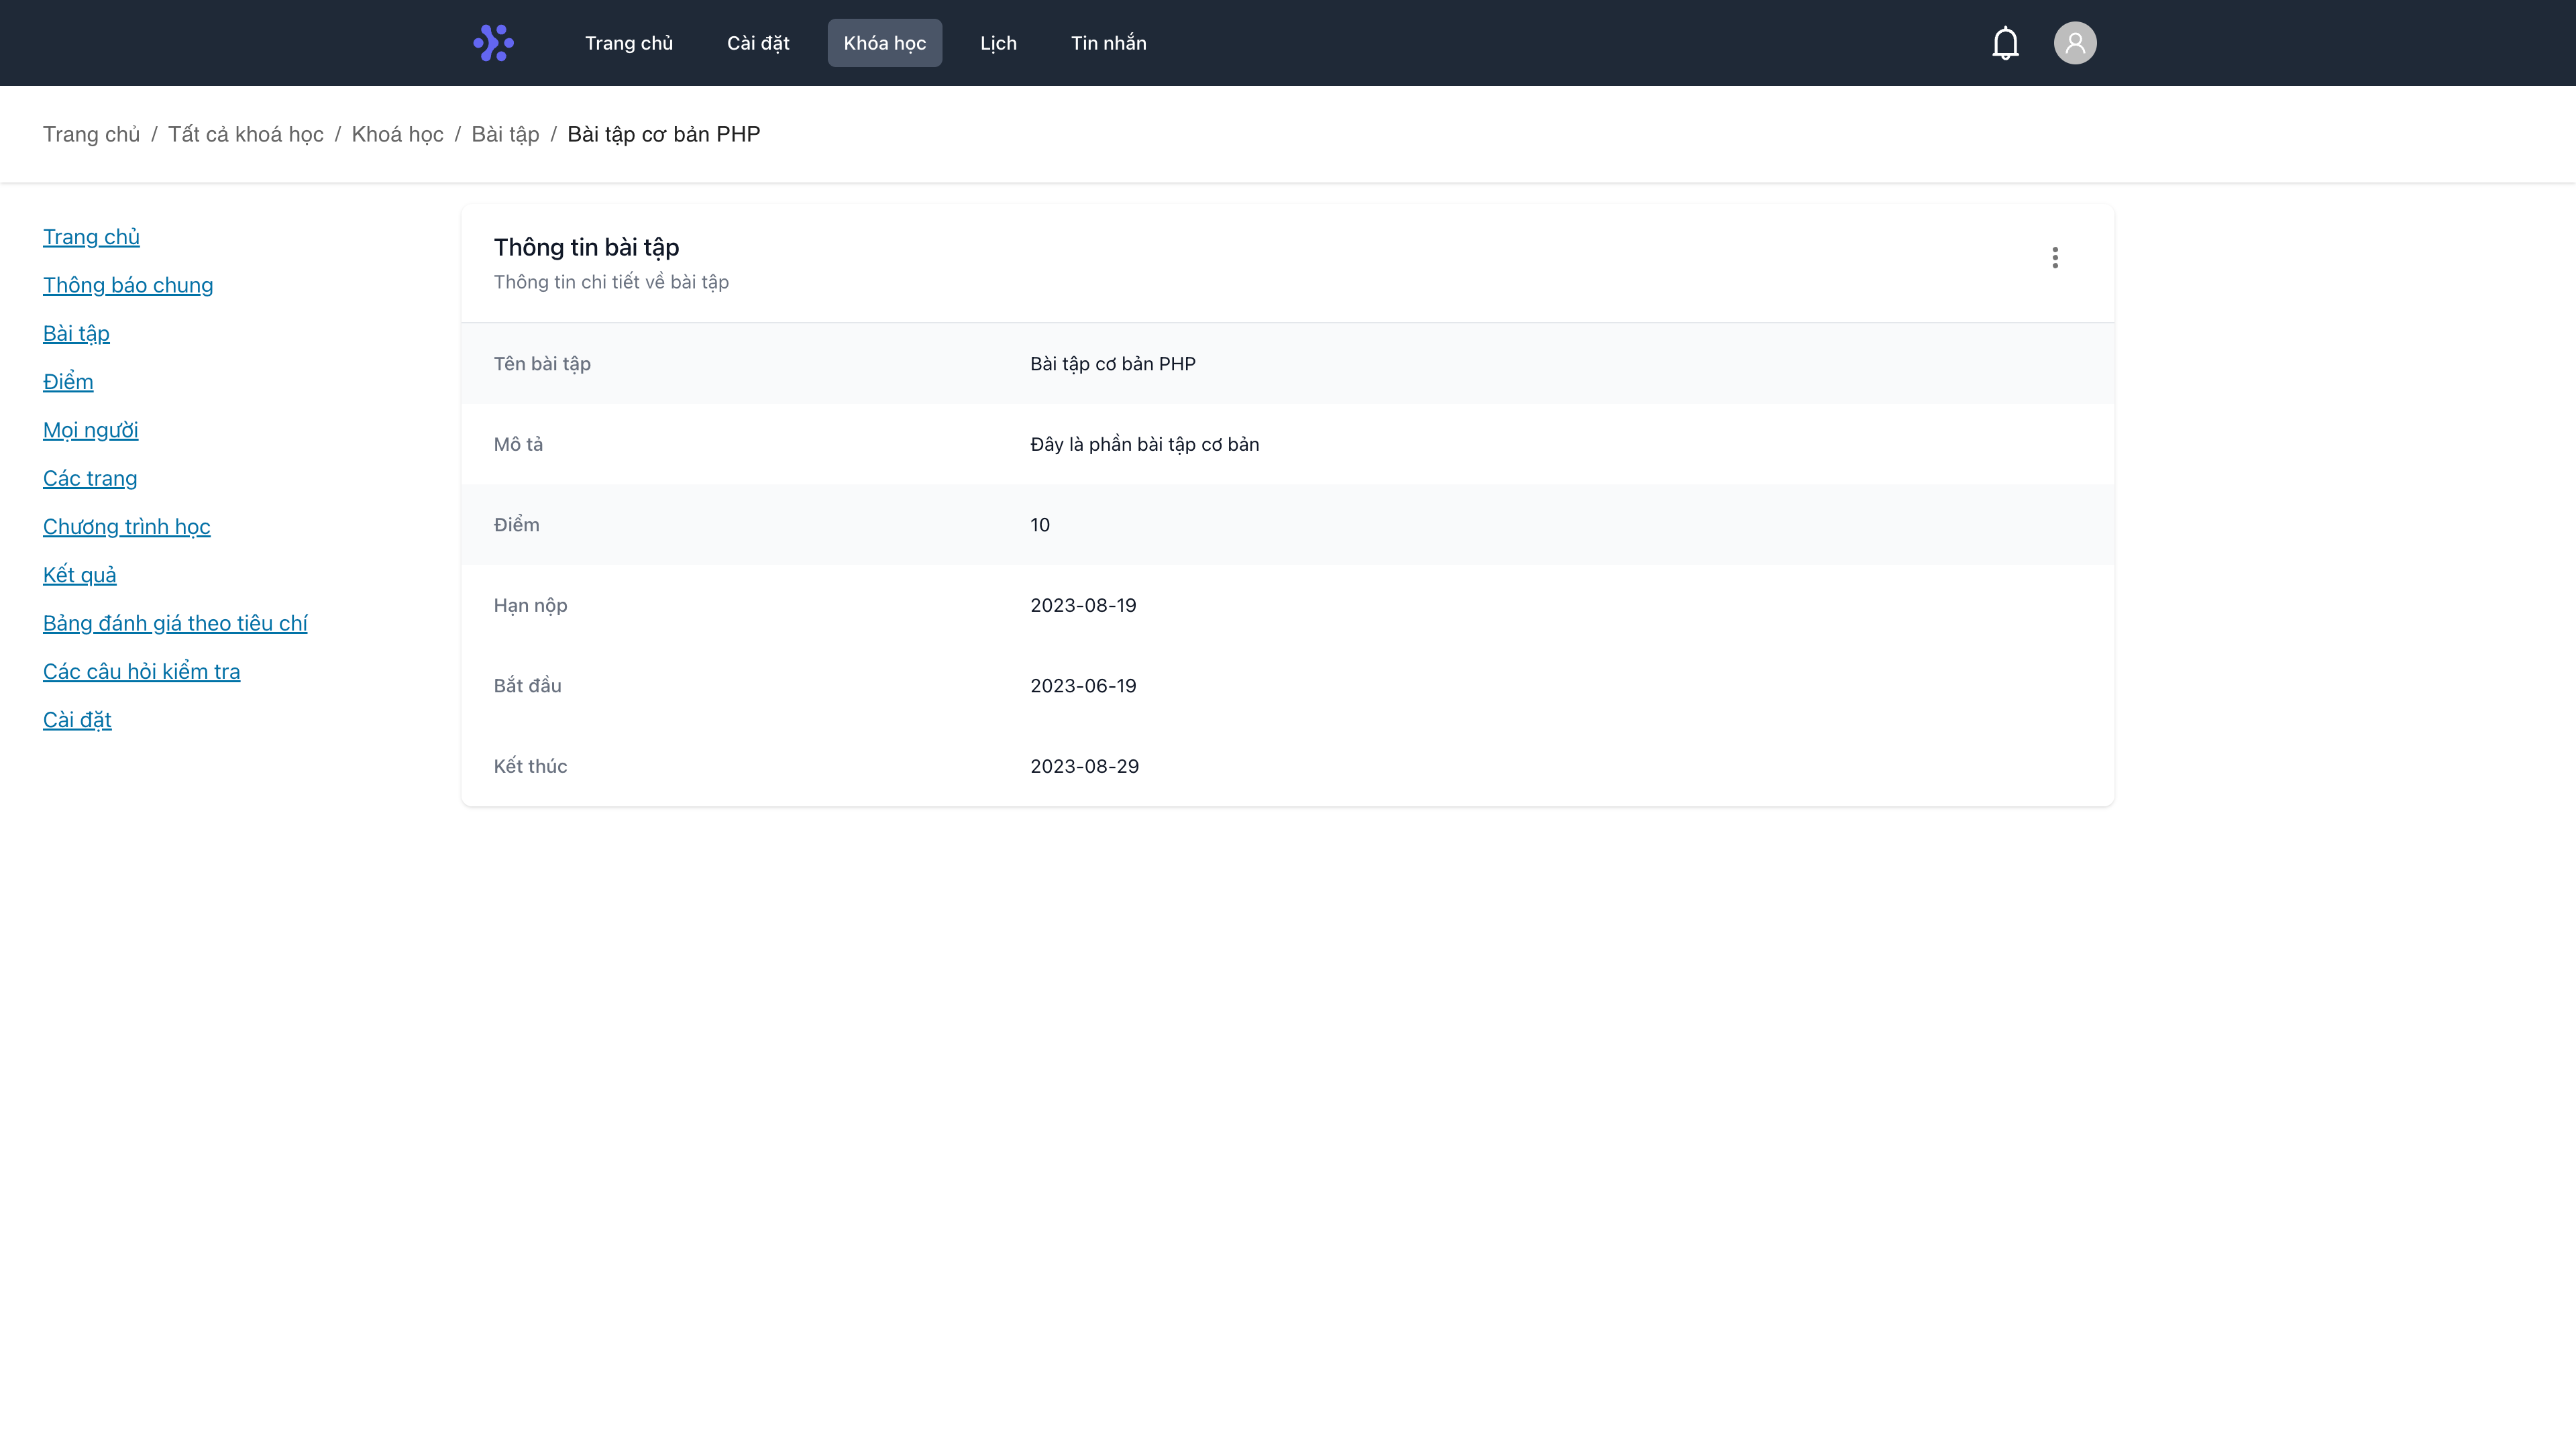
\includegraphics[width=300pt, height=200pt]{chi-tiet-bai-tap}
                    \caption{Màn hình chi tiết bài tập của phần quản trị viên}
                    \label{fig:chi-tiet-bai-tap}
                \end{figure}
                \FloatBarrier

                \item Phần chỉnh sửa bài tập của phần quản trị viên được thể hiện ở hình \ref{fig:chinh-sua-bai-tap}:
                \begin{figure}[hbt!]
                    \centering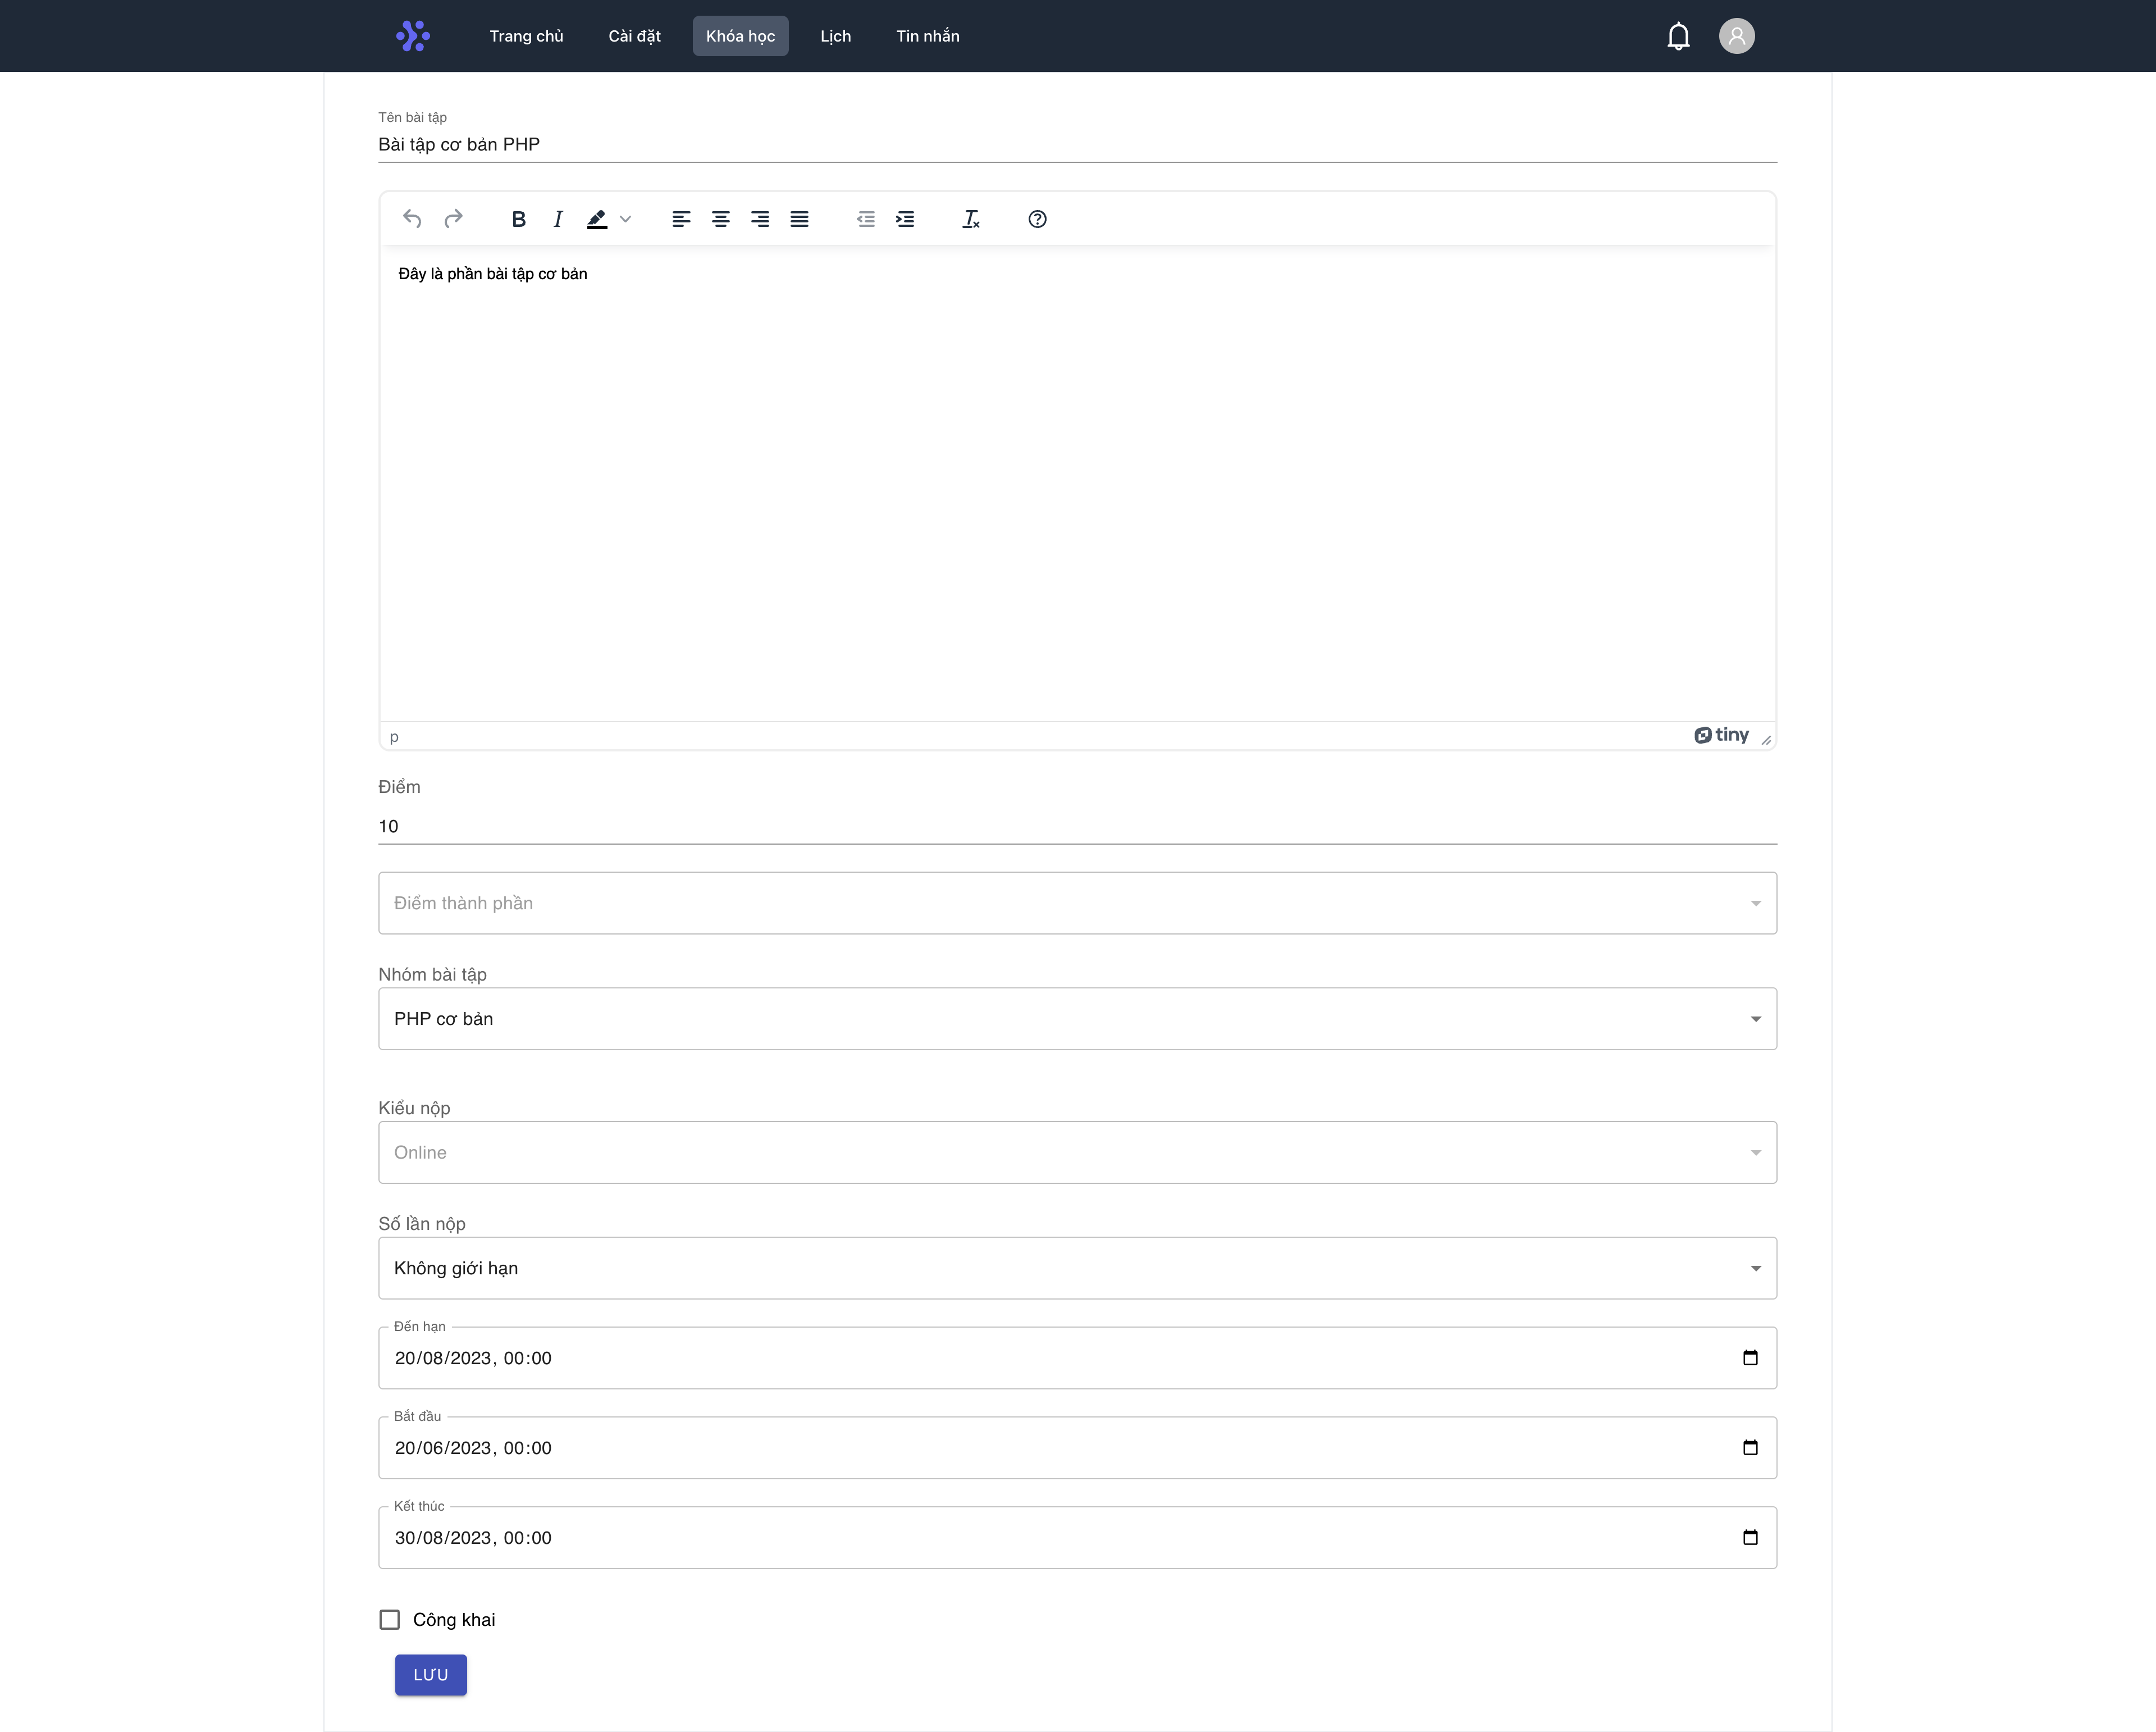
\includegraphics[width=300pt, height=200pt]{chinh-sua-bai-tap}
                    \caption{Màn hình chỉnh sửa bài tập của phần quản trị viên}
                    \label{fig:chinh-sua-bai-tap}
                \end{figure}
                \FloatBarrier

                \item Phần hiển thị điểm được thể hiện ở hình \ref{fig:hien-thi-diem}:
                \begin{figure}[hbt!]
                    \centering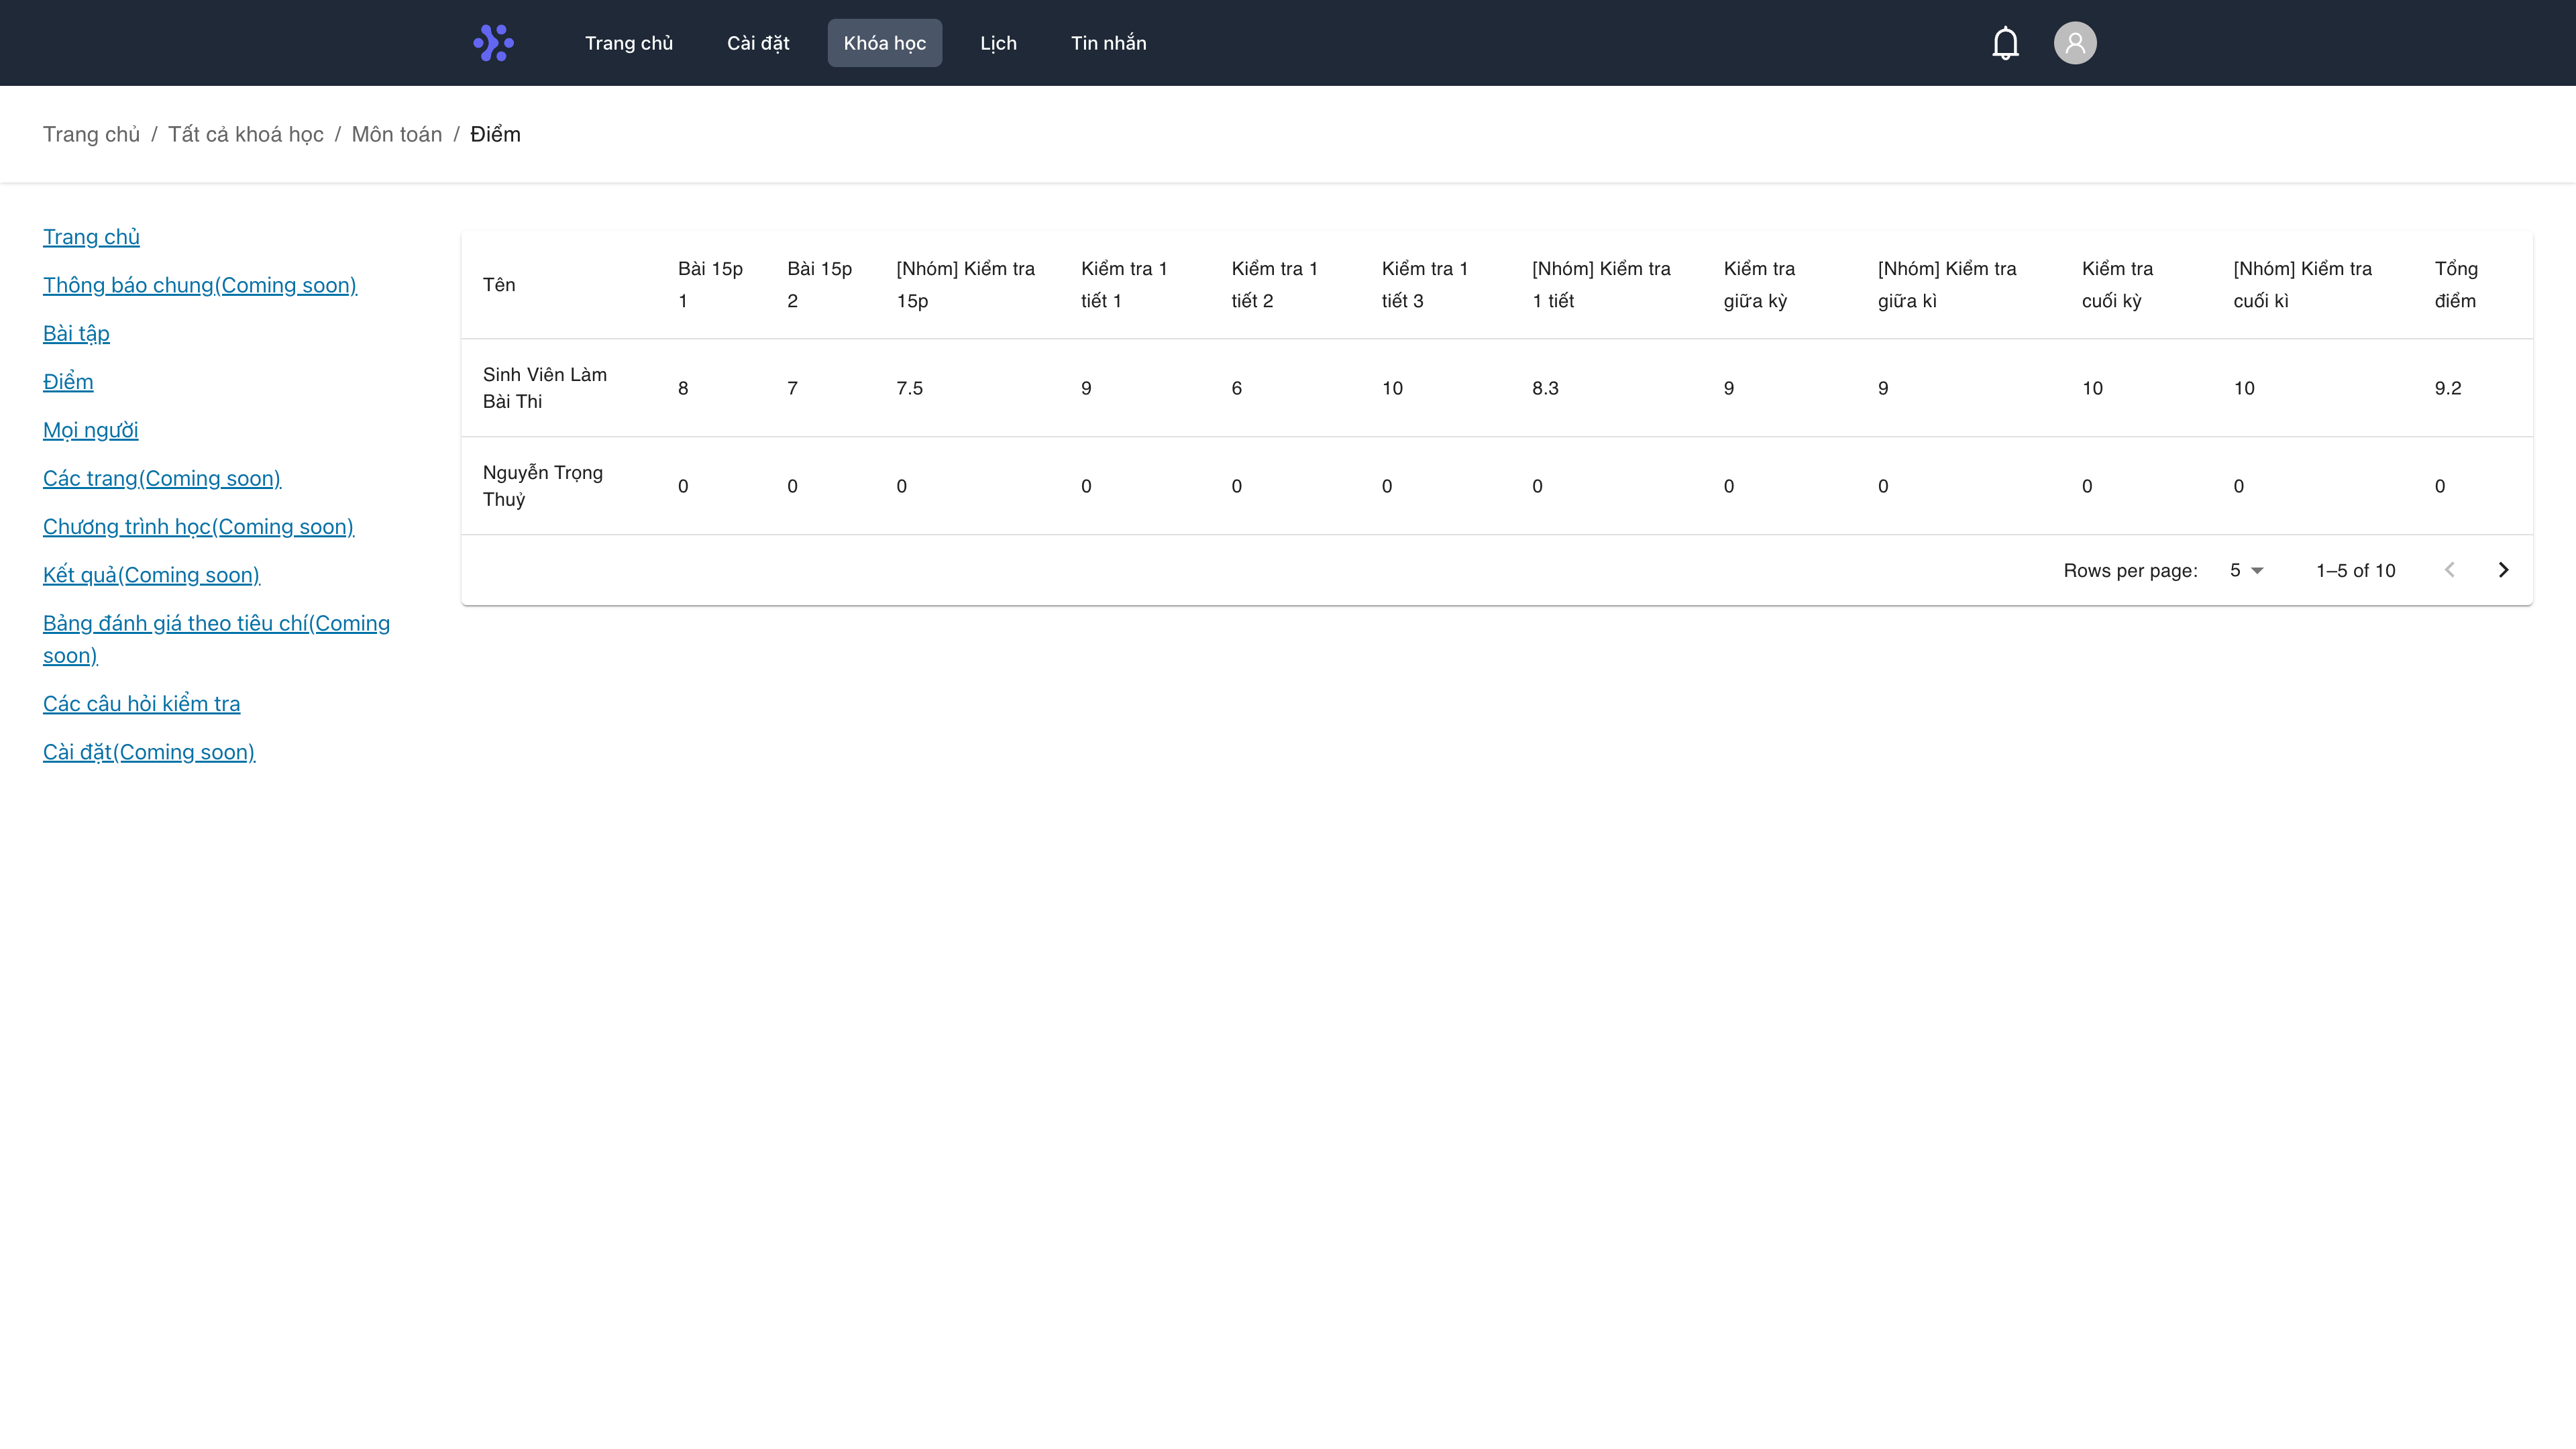
\includegraphics[width=300pt, height=200pt]{hien-thi-diem}
                    \caption{Màn hình hiển thị điểm}
                    \label{fig:hien-thi-diem}
                \end{figure}
                \FloatBarrier

                \item Phần câu hỏi kiểm tra của phần quản trị viên được thể hiện ở hình \ref{fig:cau-hoi-kiem-tra}:
                \begin{figure}[hbt!]
                    \centering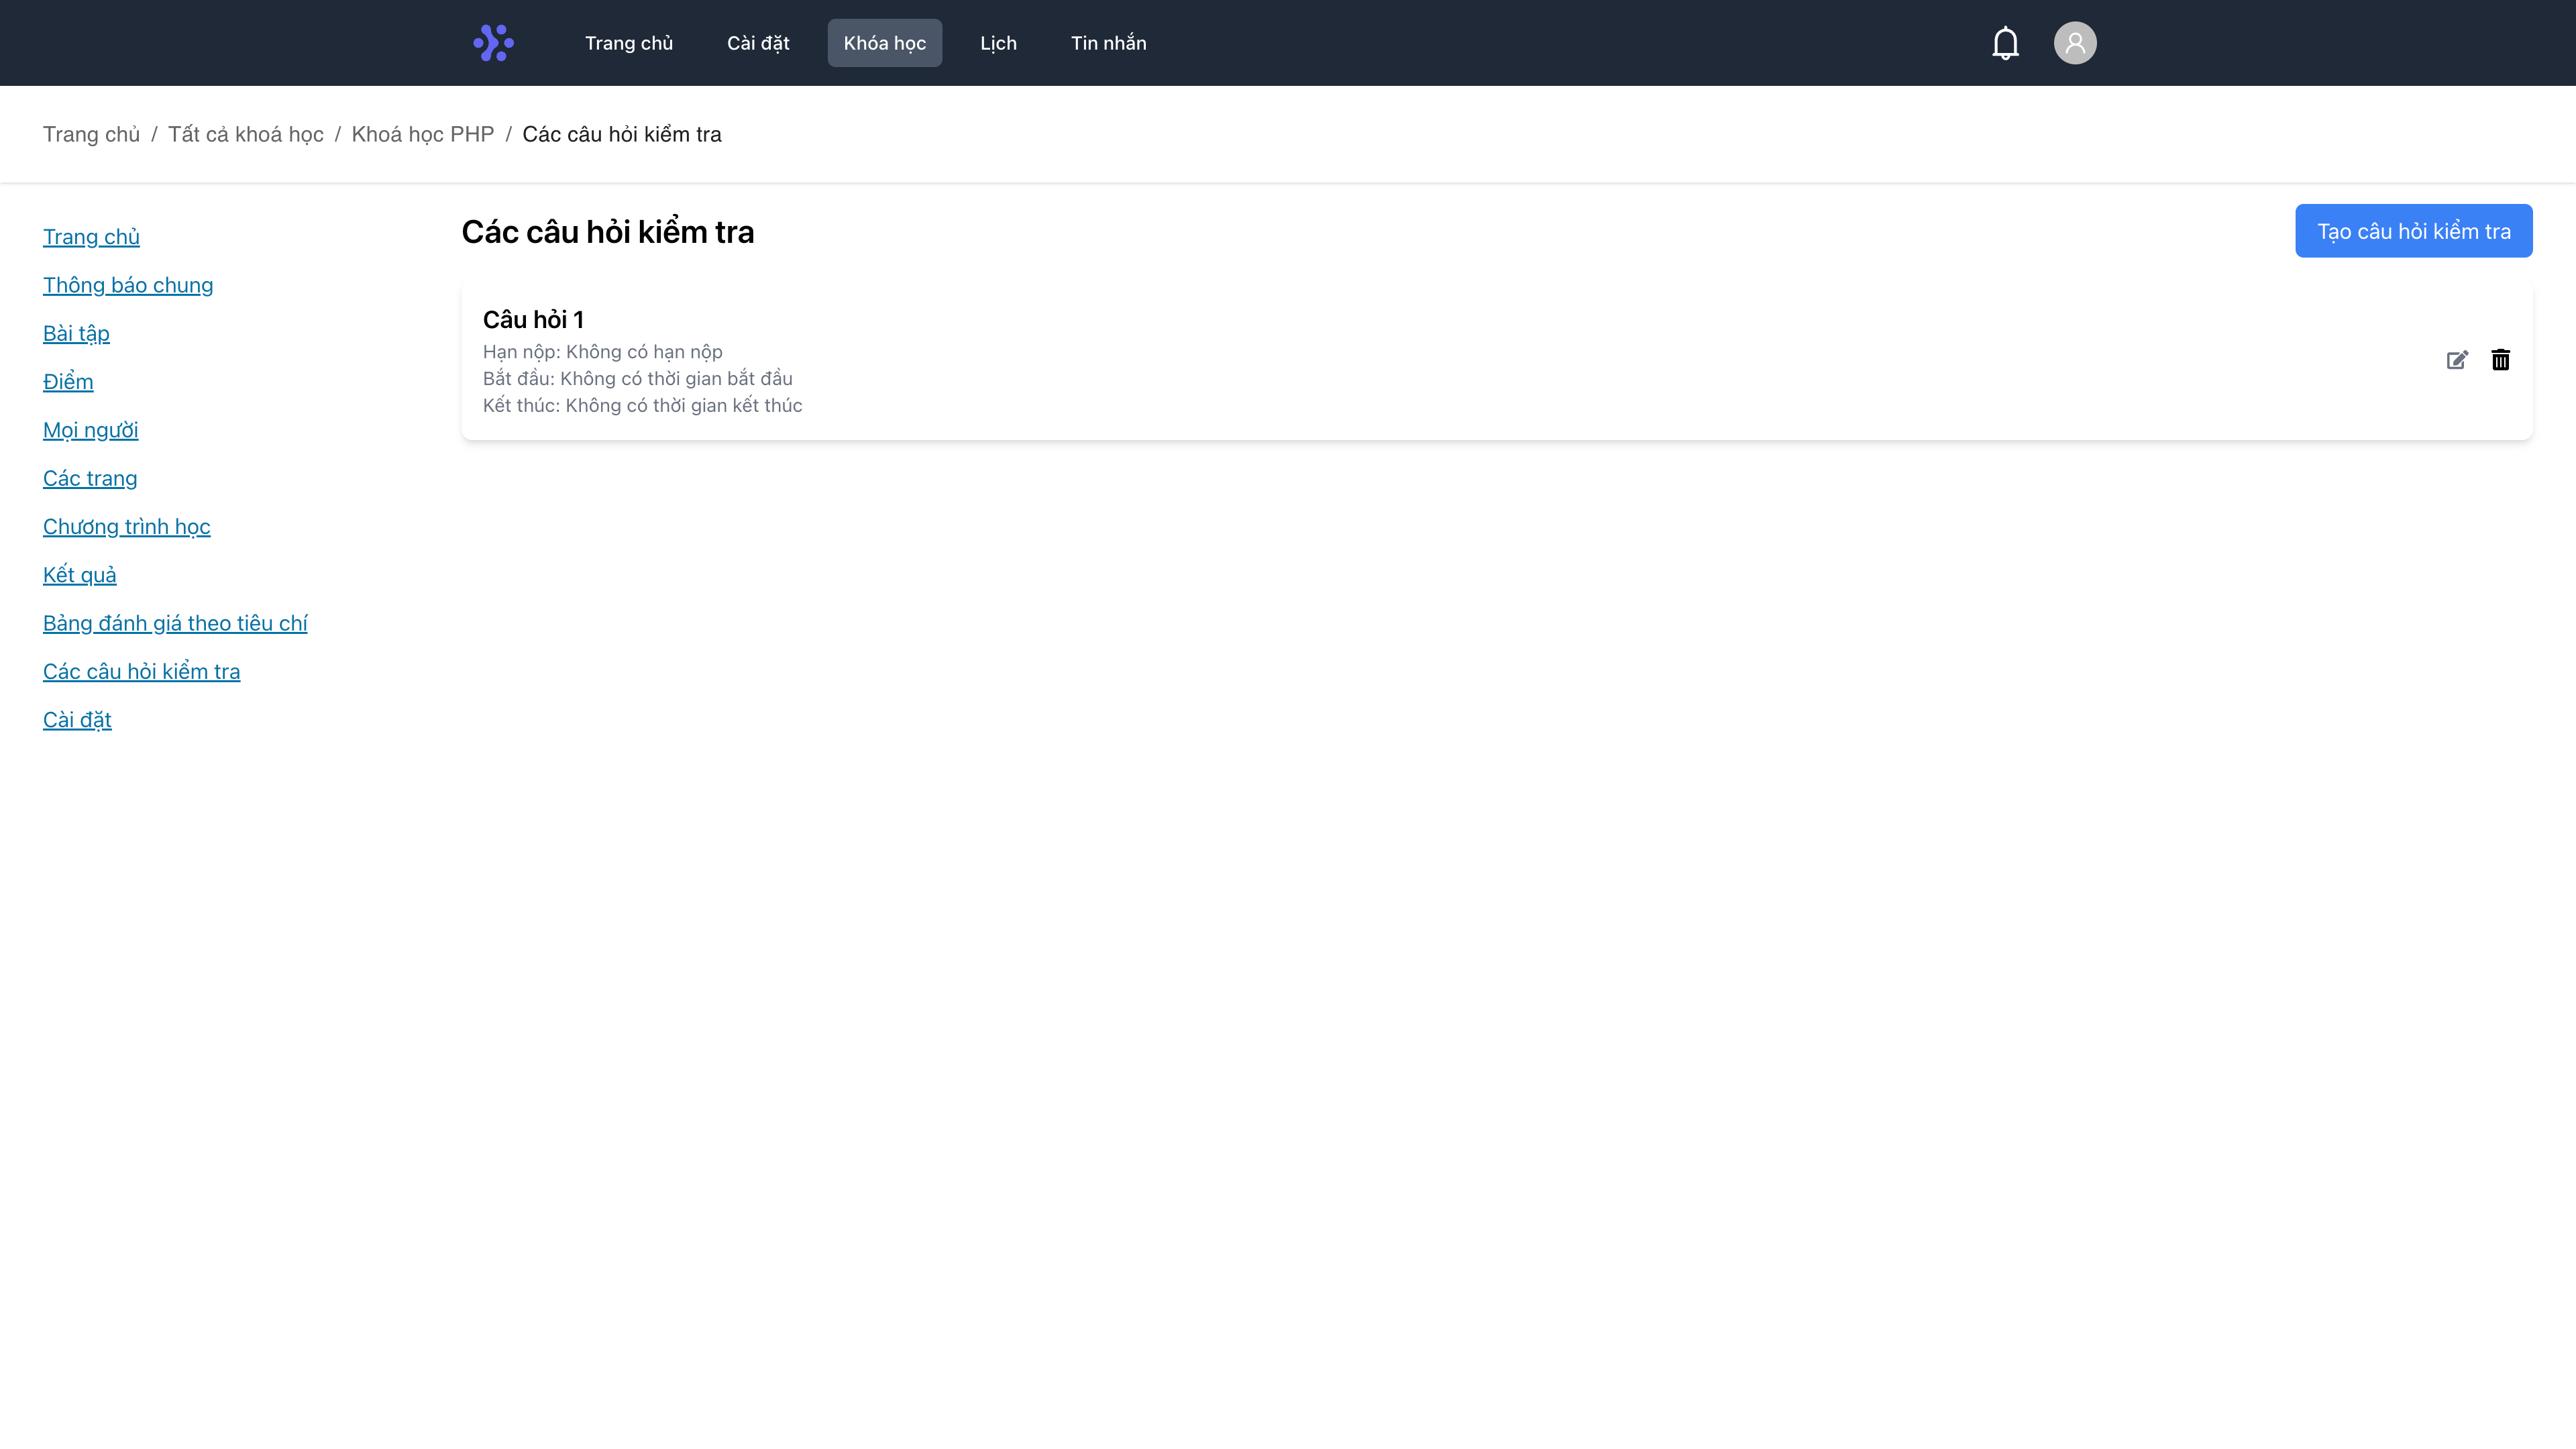
\includegraphics[width=300pt, height=200pt]{cau-hoi-kiem-tra}
                    \caption{Màn hình câu hỏi kiểm tra của phần quản trị viên}
                    \label{fig:cau-hoi-kiem-tra}
                \end{figure}
                \FloatBarrier

                \item Phần tạo câu hỏi kiểm tra của phần quản trị viên được thể hiện ở hình \ref{fig:tao-cau-hoi-kiem-tra}:
                \begin{figure}[hbt!]
                    \centering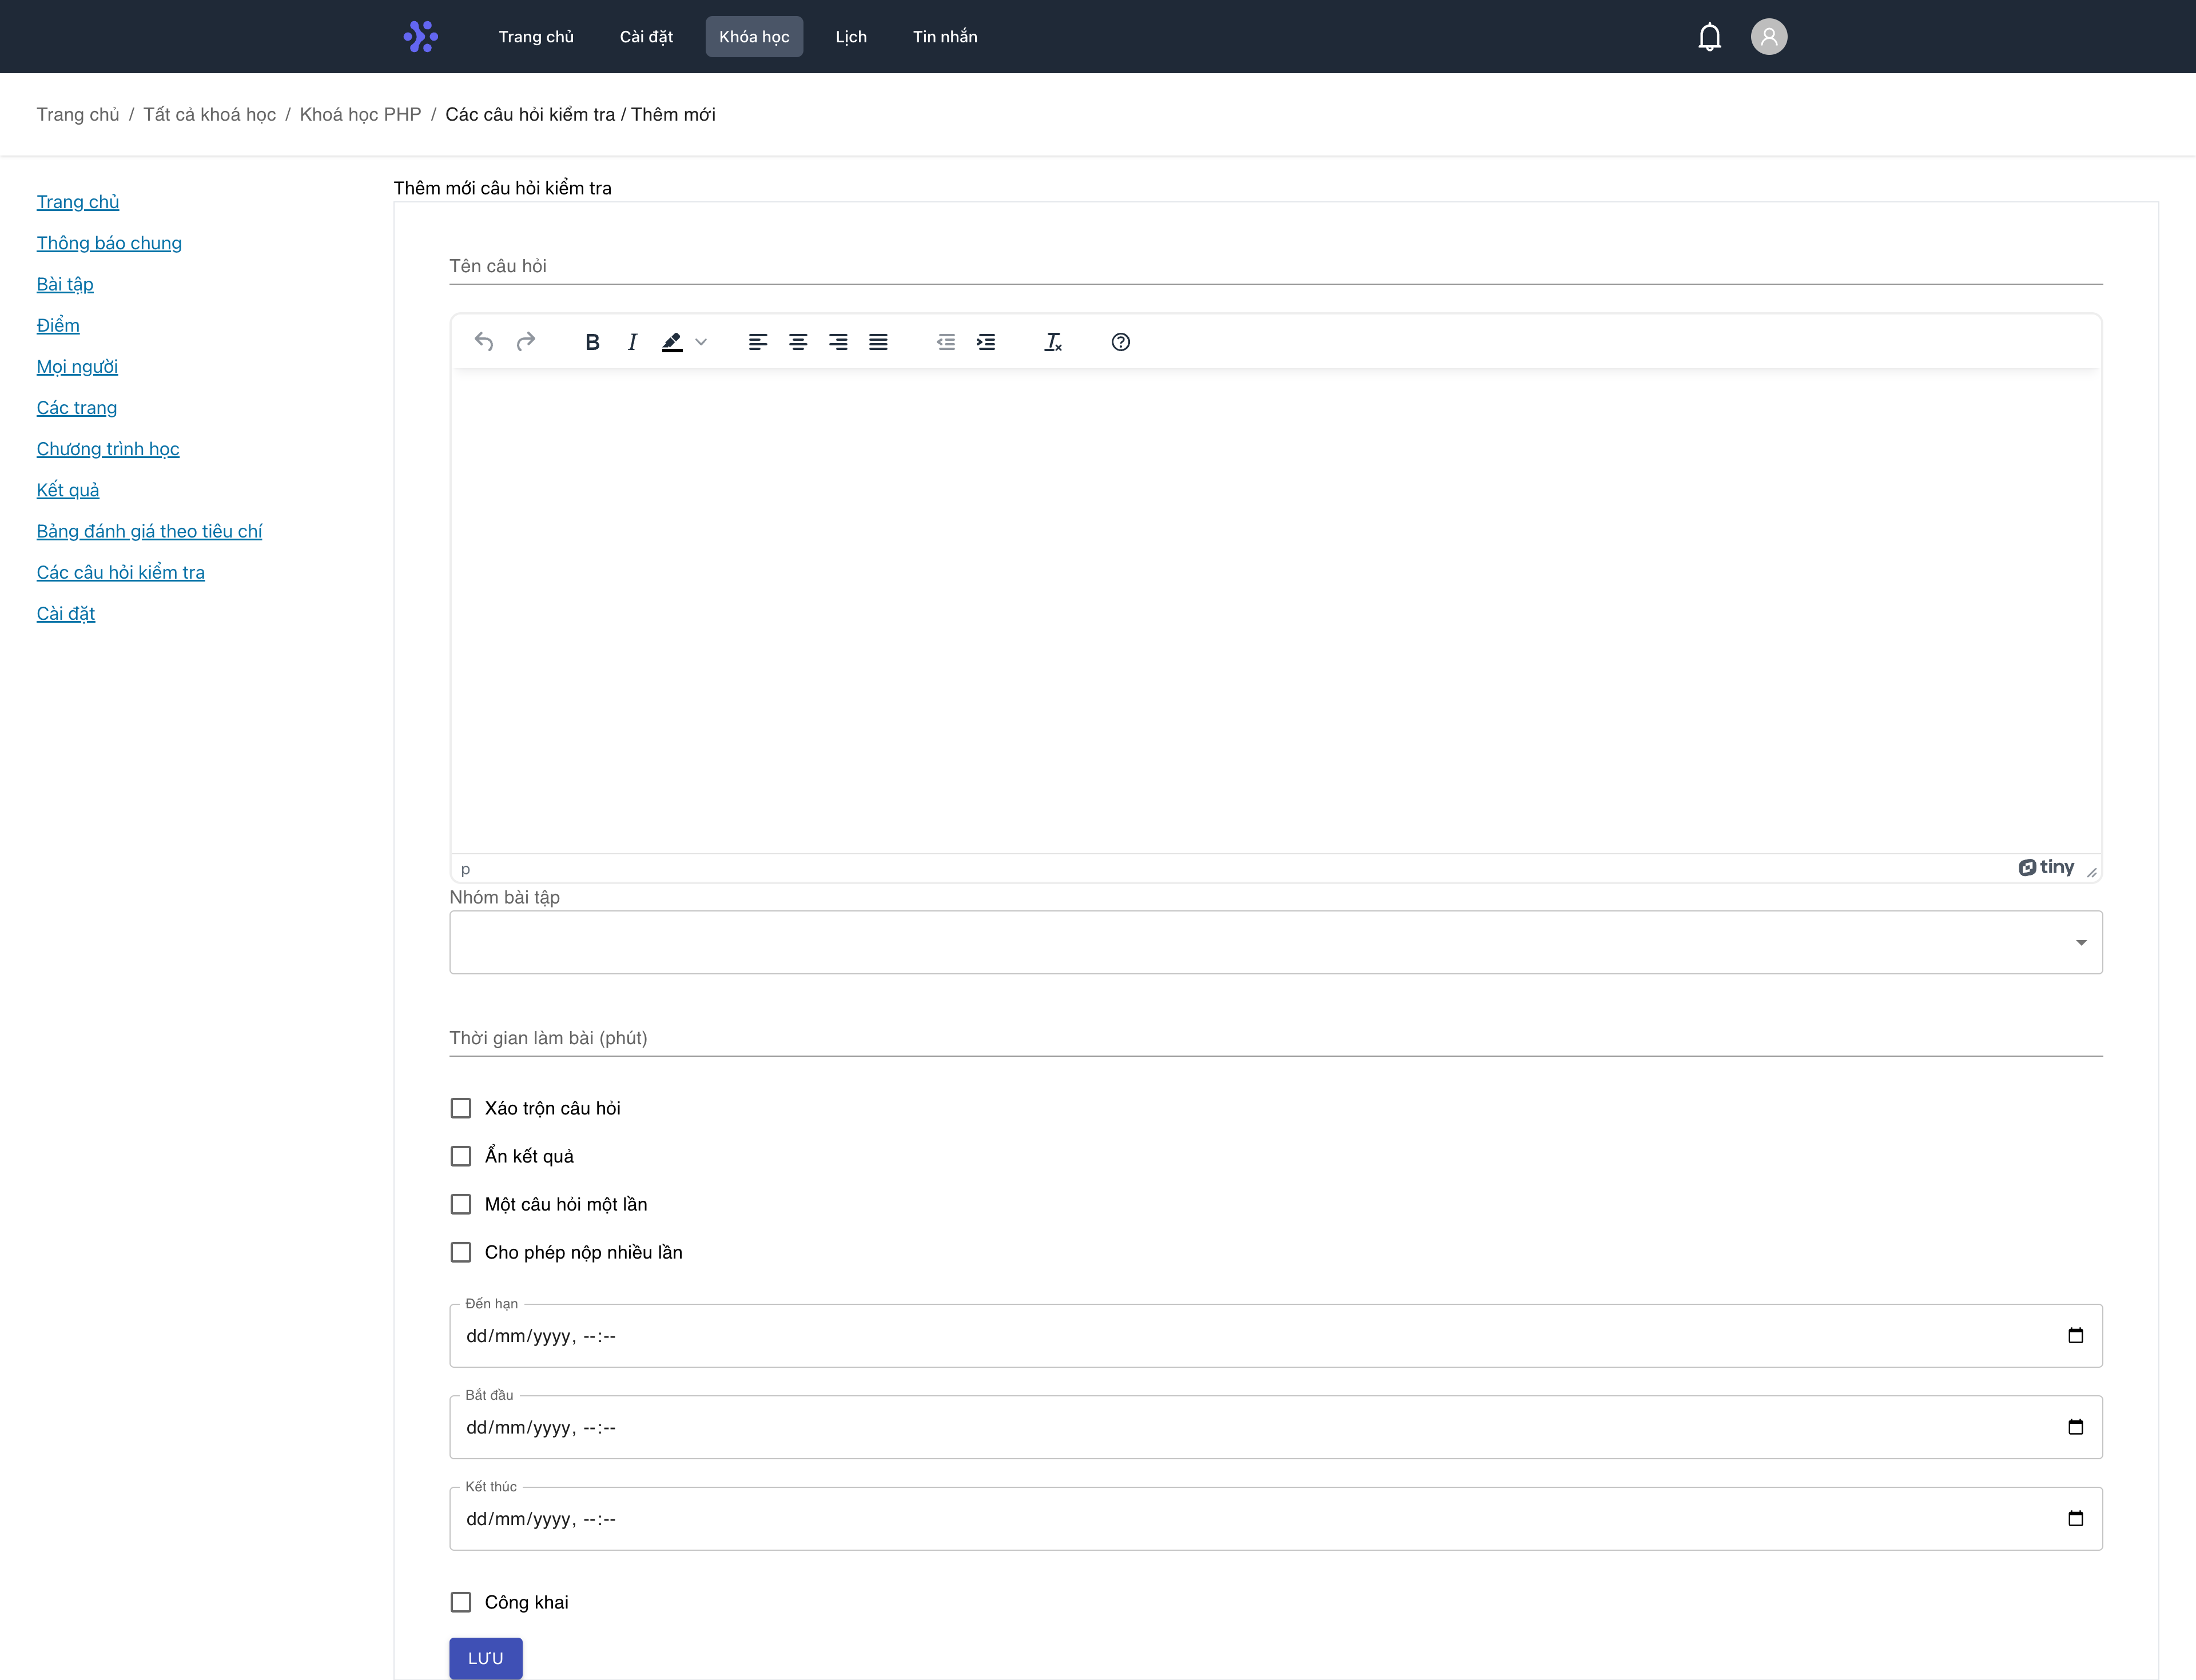
\includegraphics[width=300pt, height=200pt]{tao-cau-hoi-kiem-tra}
                    \caption{Màn hình tạo câu hỏi kiểm tra của phần quản trị viên}
                    \label{fig:tao-cau-hoi-kiem-tra}
                \end{figure}
                \FloatBarrier

                \item Phần chỉnh sửa câu hỏi kiểm tra của phần quản trị viên được thể hiện ở hình \ref{fig:chinh-sua-cau-hoi-kiem-tra}:
                \begin{figure}[hbt!]
                    \centering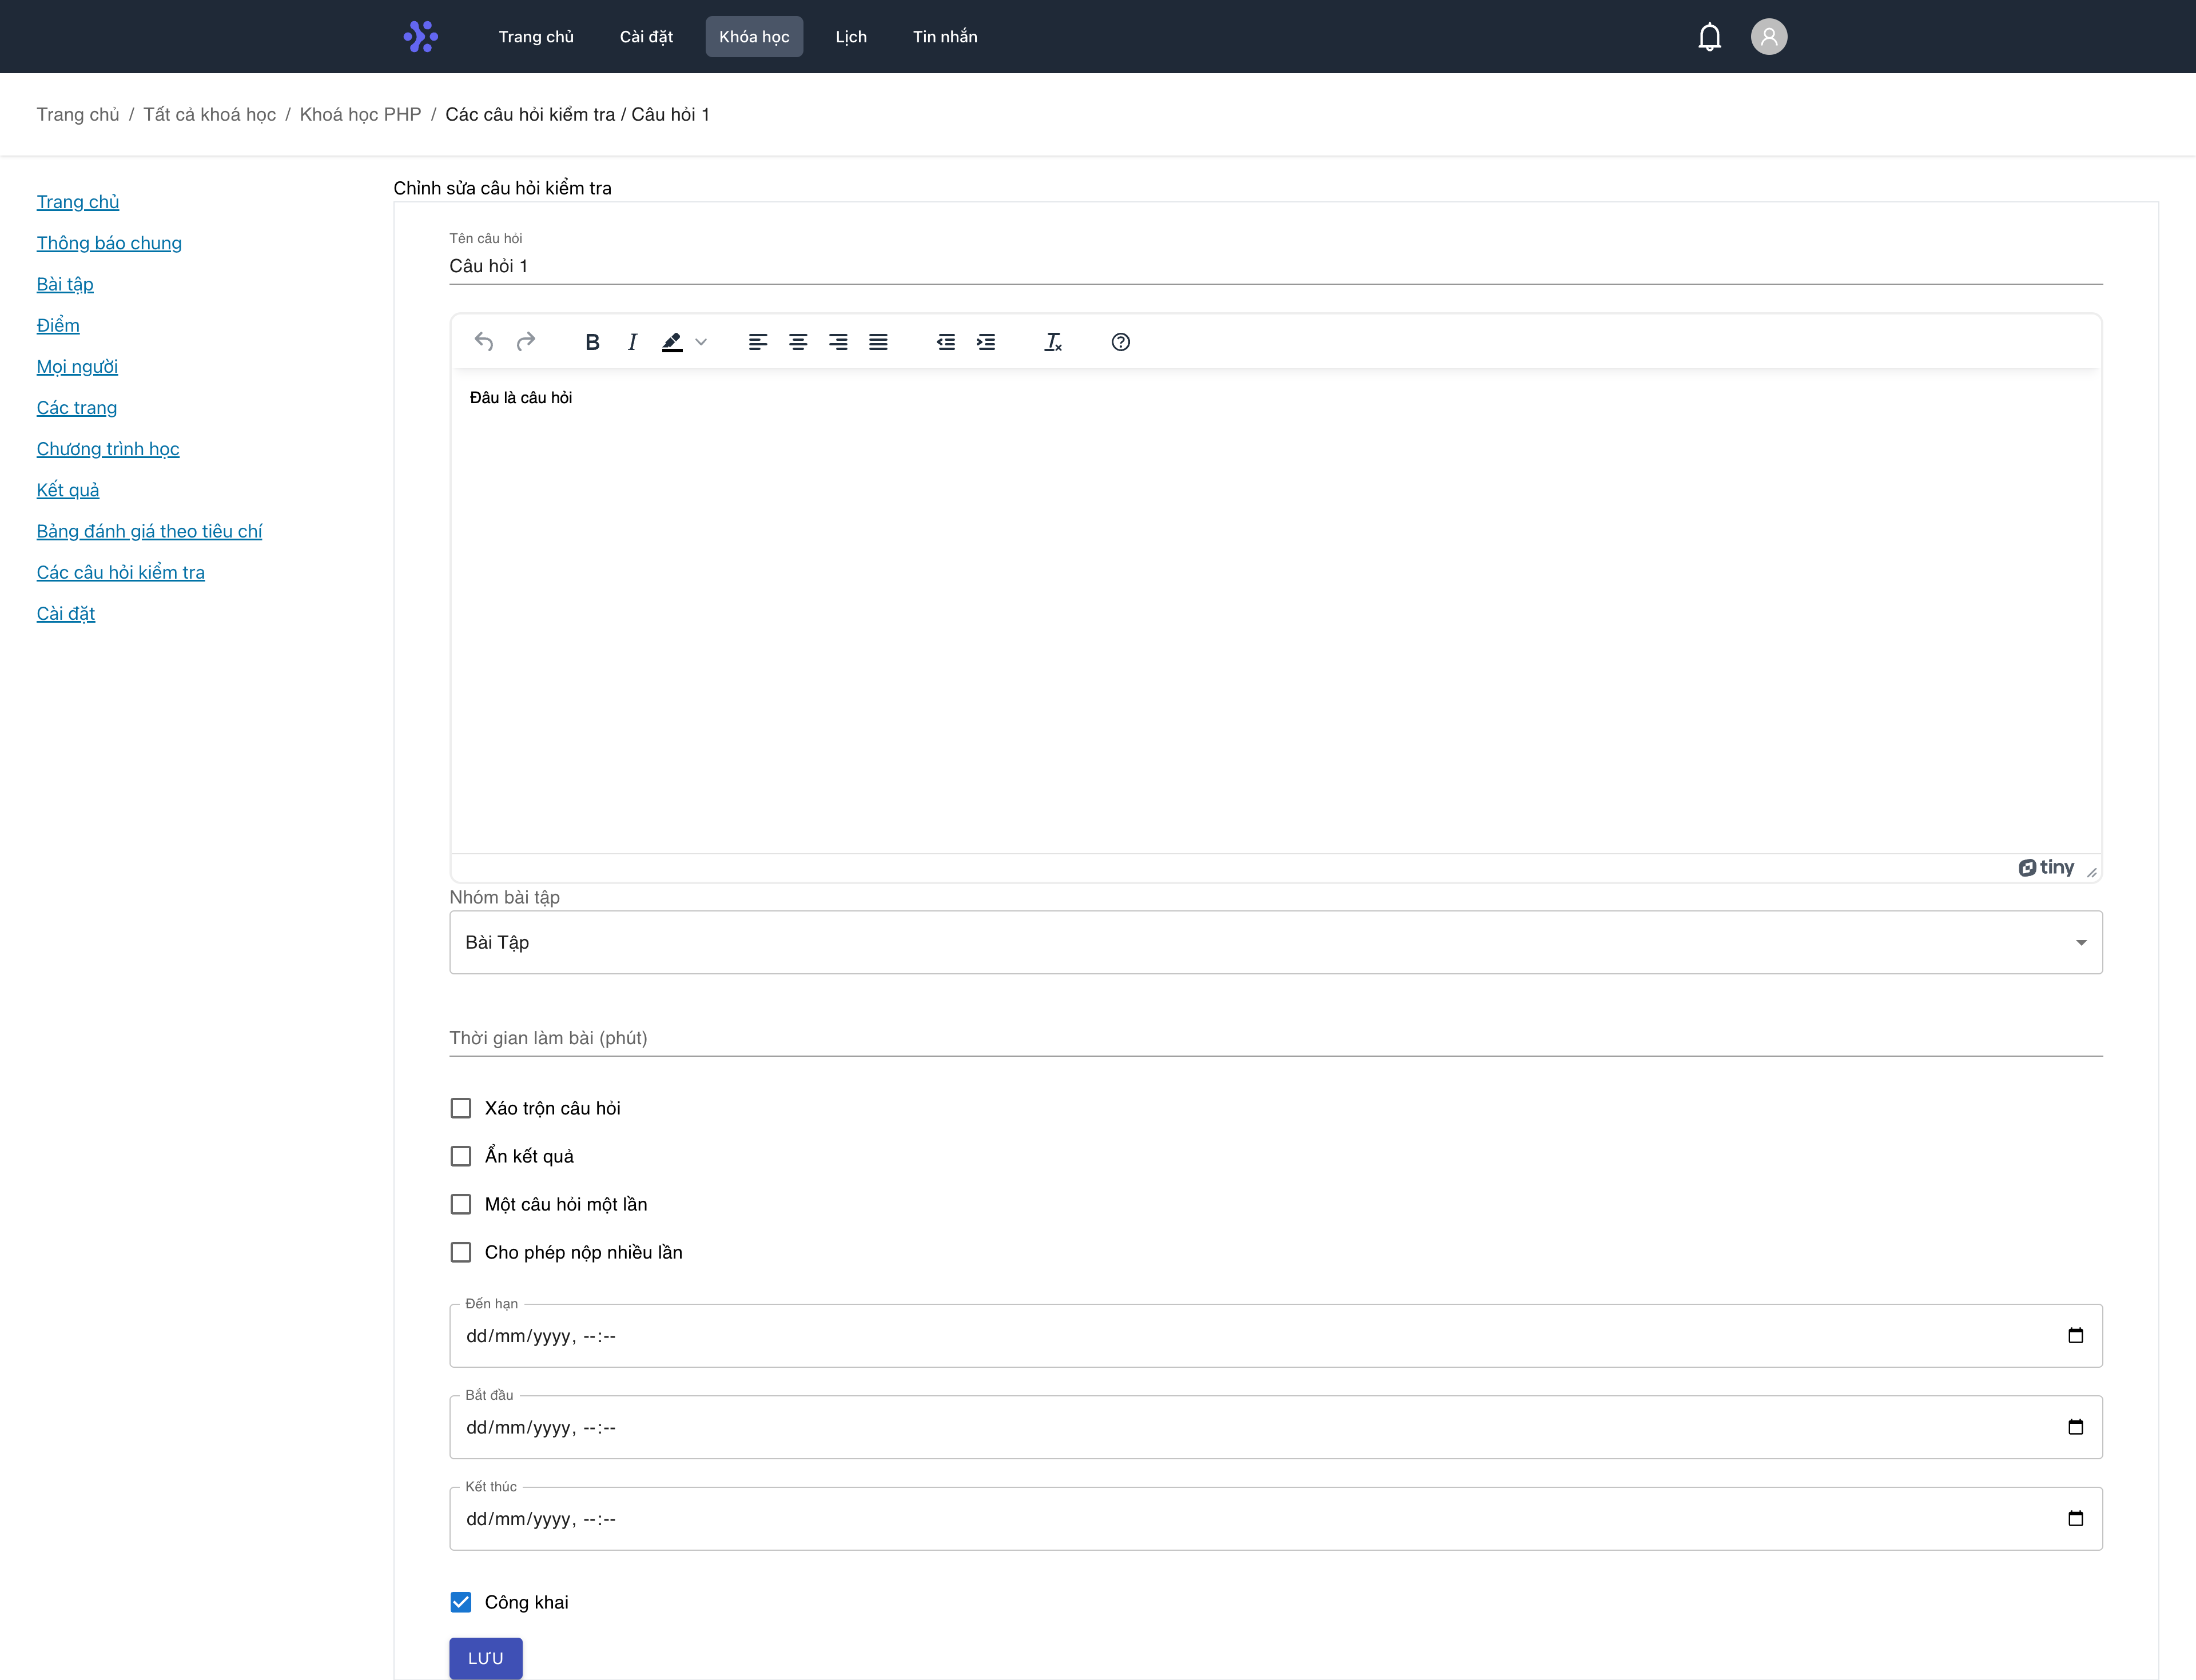
\includegraphics[width=300pt, height=200pt]{chinh-sua-cau-hoi-kiem-tra}
                    \caption{Màn hình chỉnh sửa câu hỏi kiểm tra của phần quản trị viên}
                    \label{fig:chinh-sua-cau-hoi-kiem-tra}
                \end{figure}
                \FloatBarrier

                \item Phần tạo câu hỏi trong câu hỏi kiểm tra của phần quản trị viên được thể hiện ở hình \ref{fig:tao-cau-hoi-trong-cau-hoi-kiem-tra}:
                \begin{figure}[hbt!]
                    \centering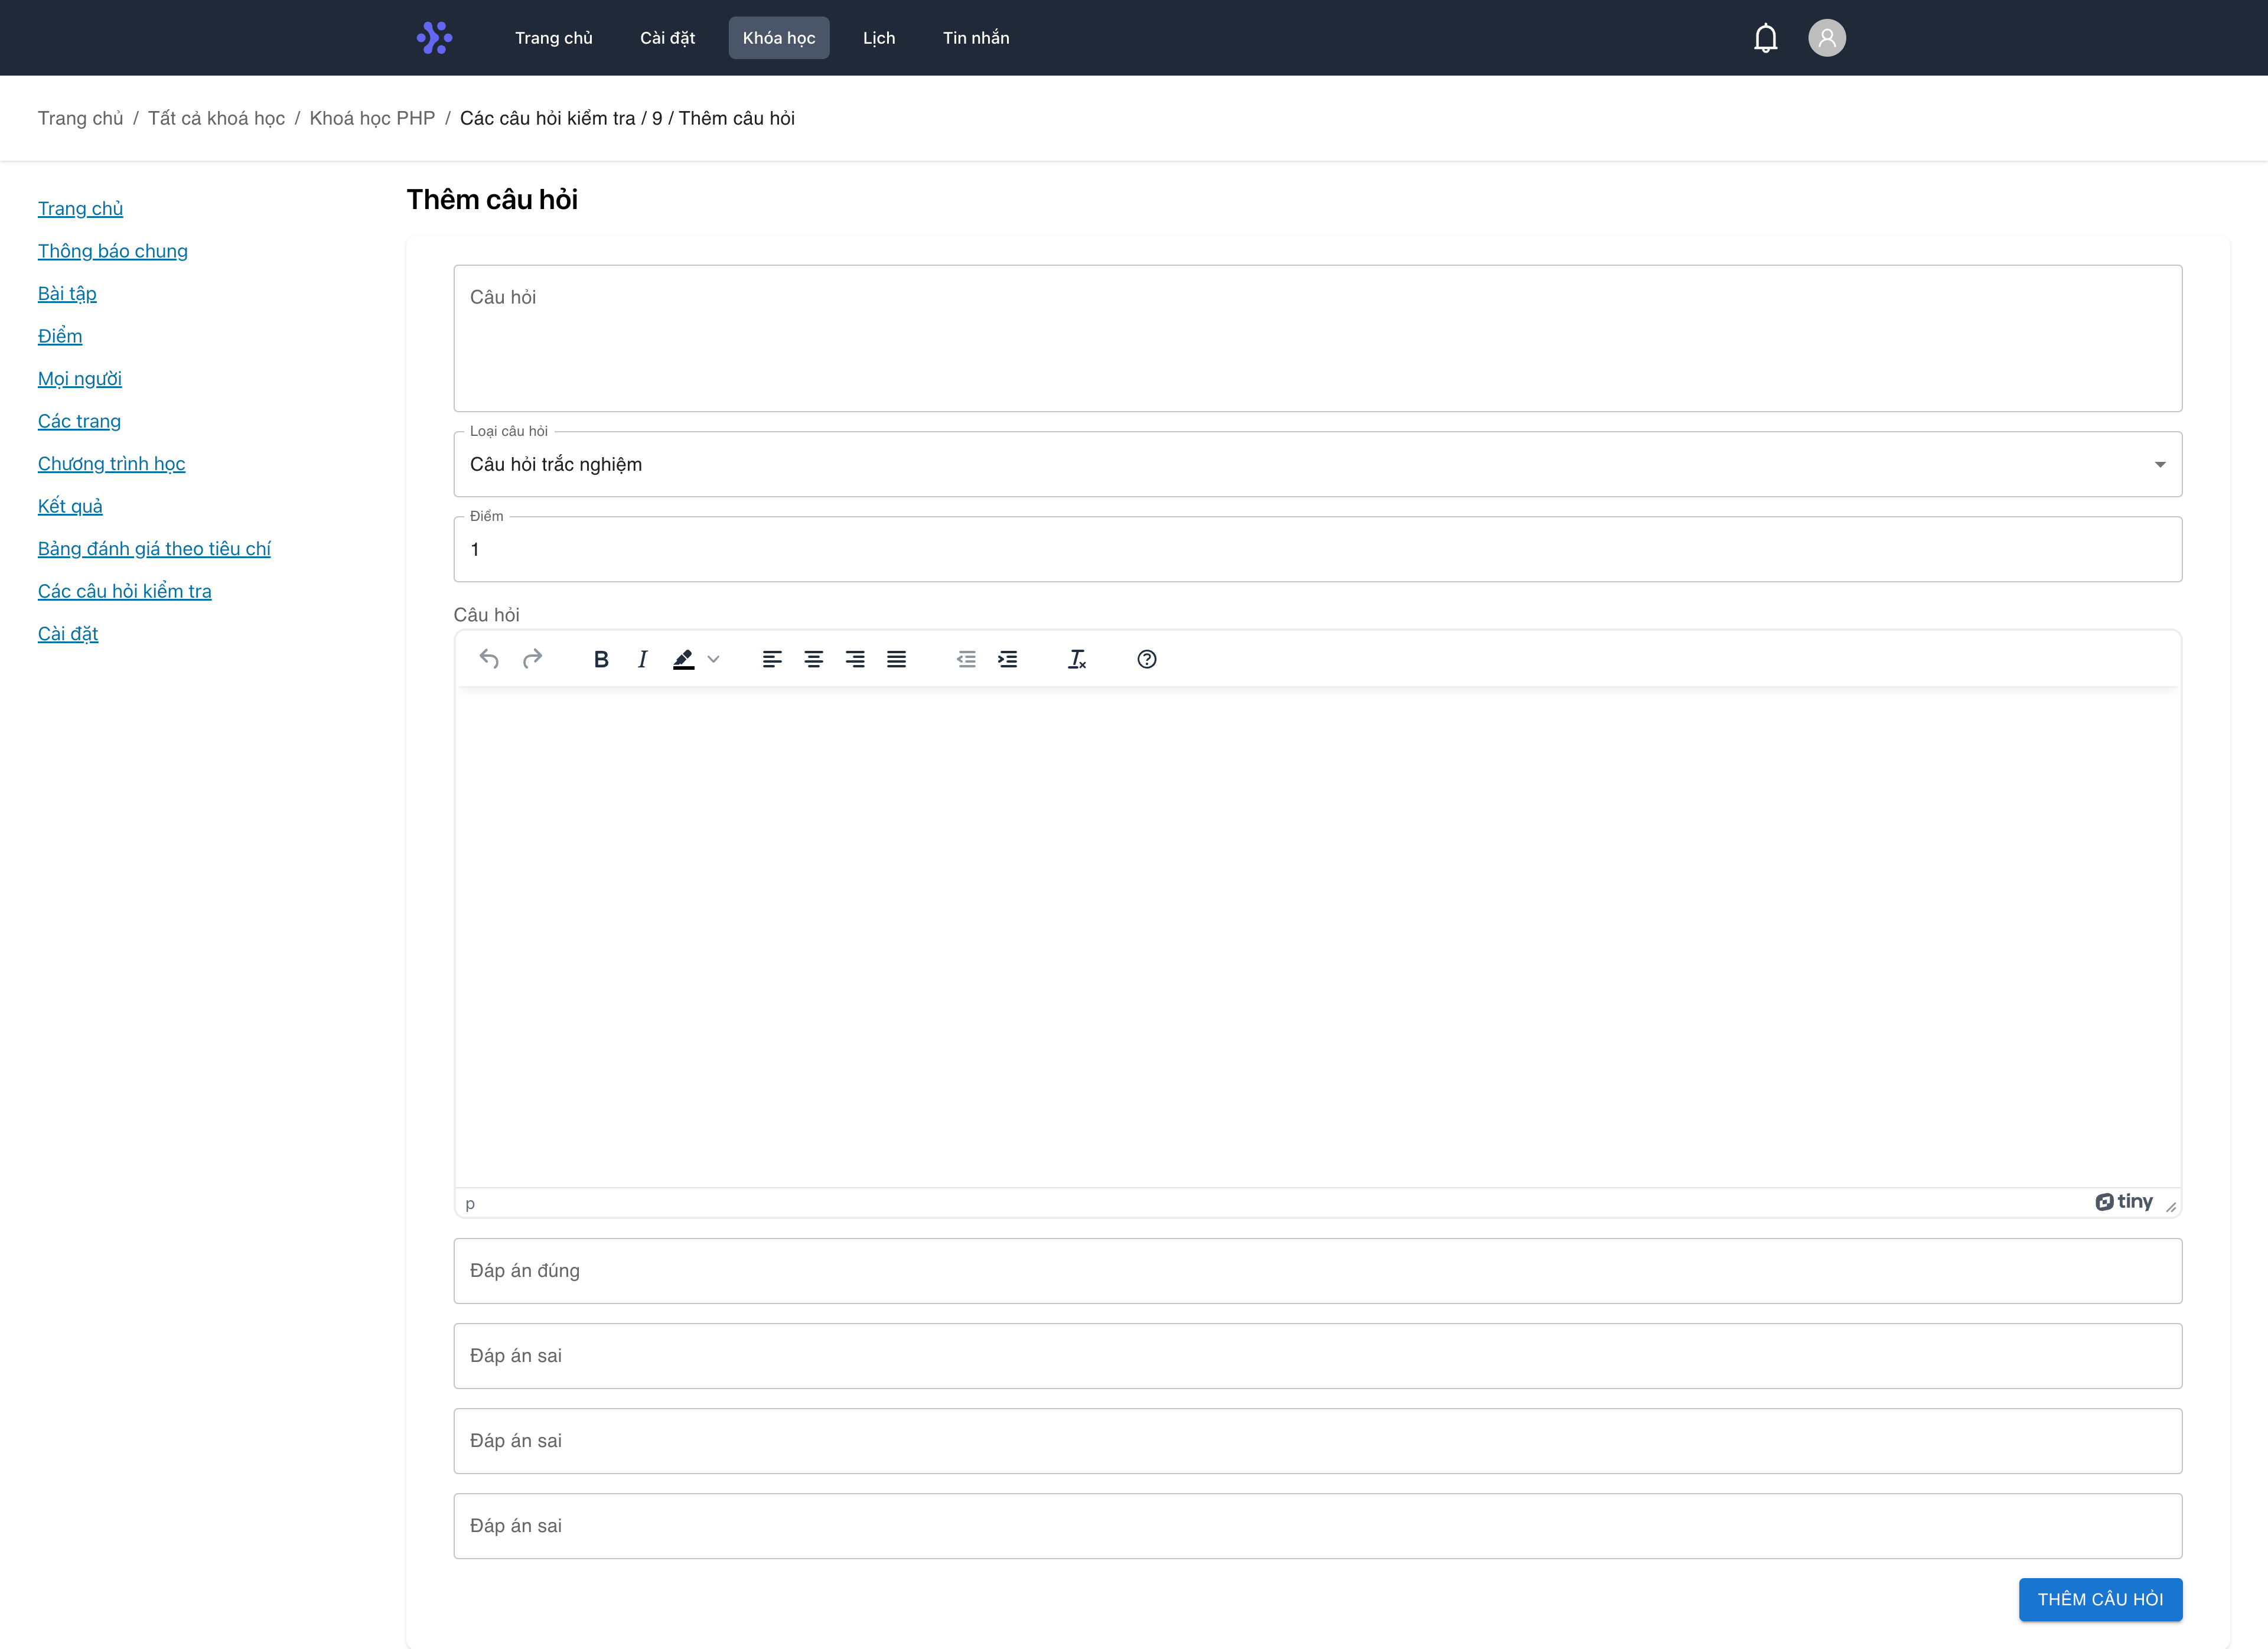
\includegraphics[width=300pt, height=200pt]{tao-cau-hoi-trong-cau-hoi-kiem-tra}
                    \caption{Màn hình tạo câu hỏi trong câu hỏi kiểm tra của phần quản trị viên}
                    \label{fig:tao-cau-hoi-trong-cau-hoi-kiem-tra}
                \end{figure}
                \FloatBarrier

                \item Phần chỉnh sửa câu hỏi trong câu hỏi kiểm tra của phần quản trị viên được thể hiện ở hình \ref{fig:chinh-sua-cau-hoi-trong-cau-hoi-kiem-tra}:
                \begin{figure}[hbt!]
                    \centering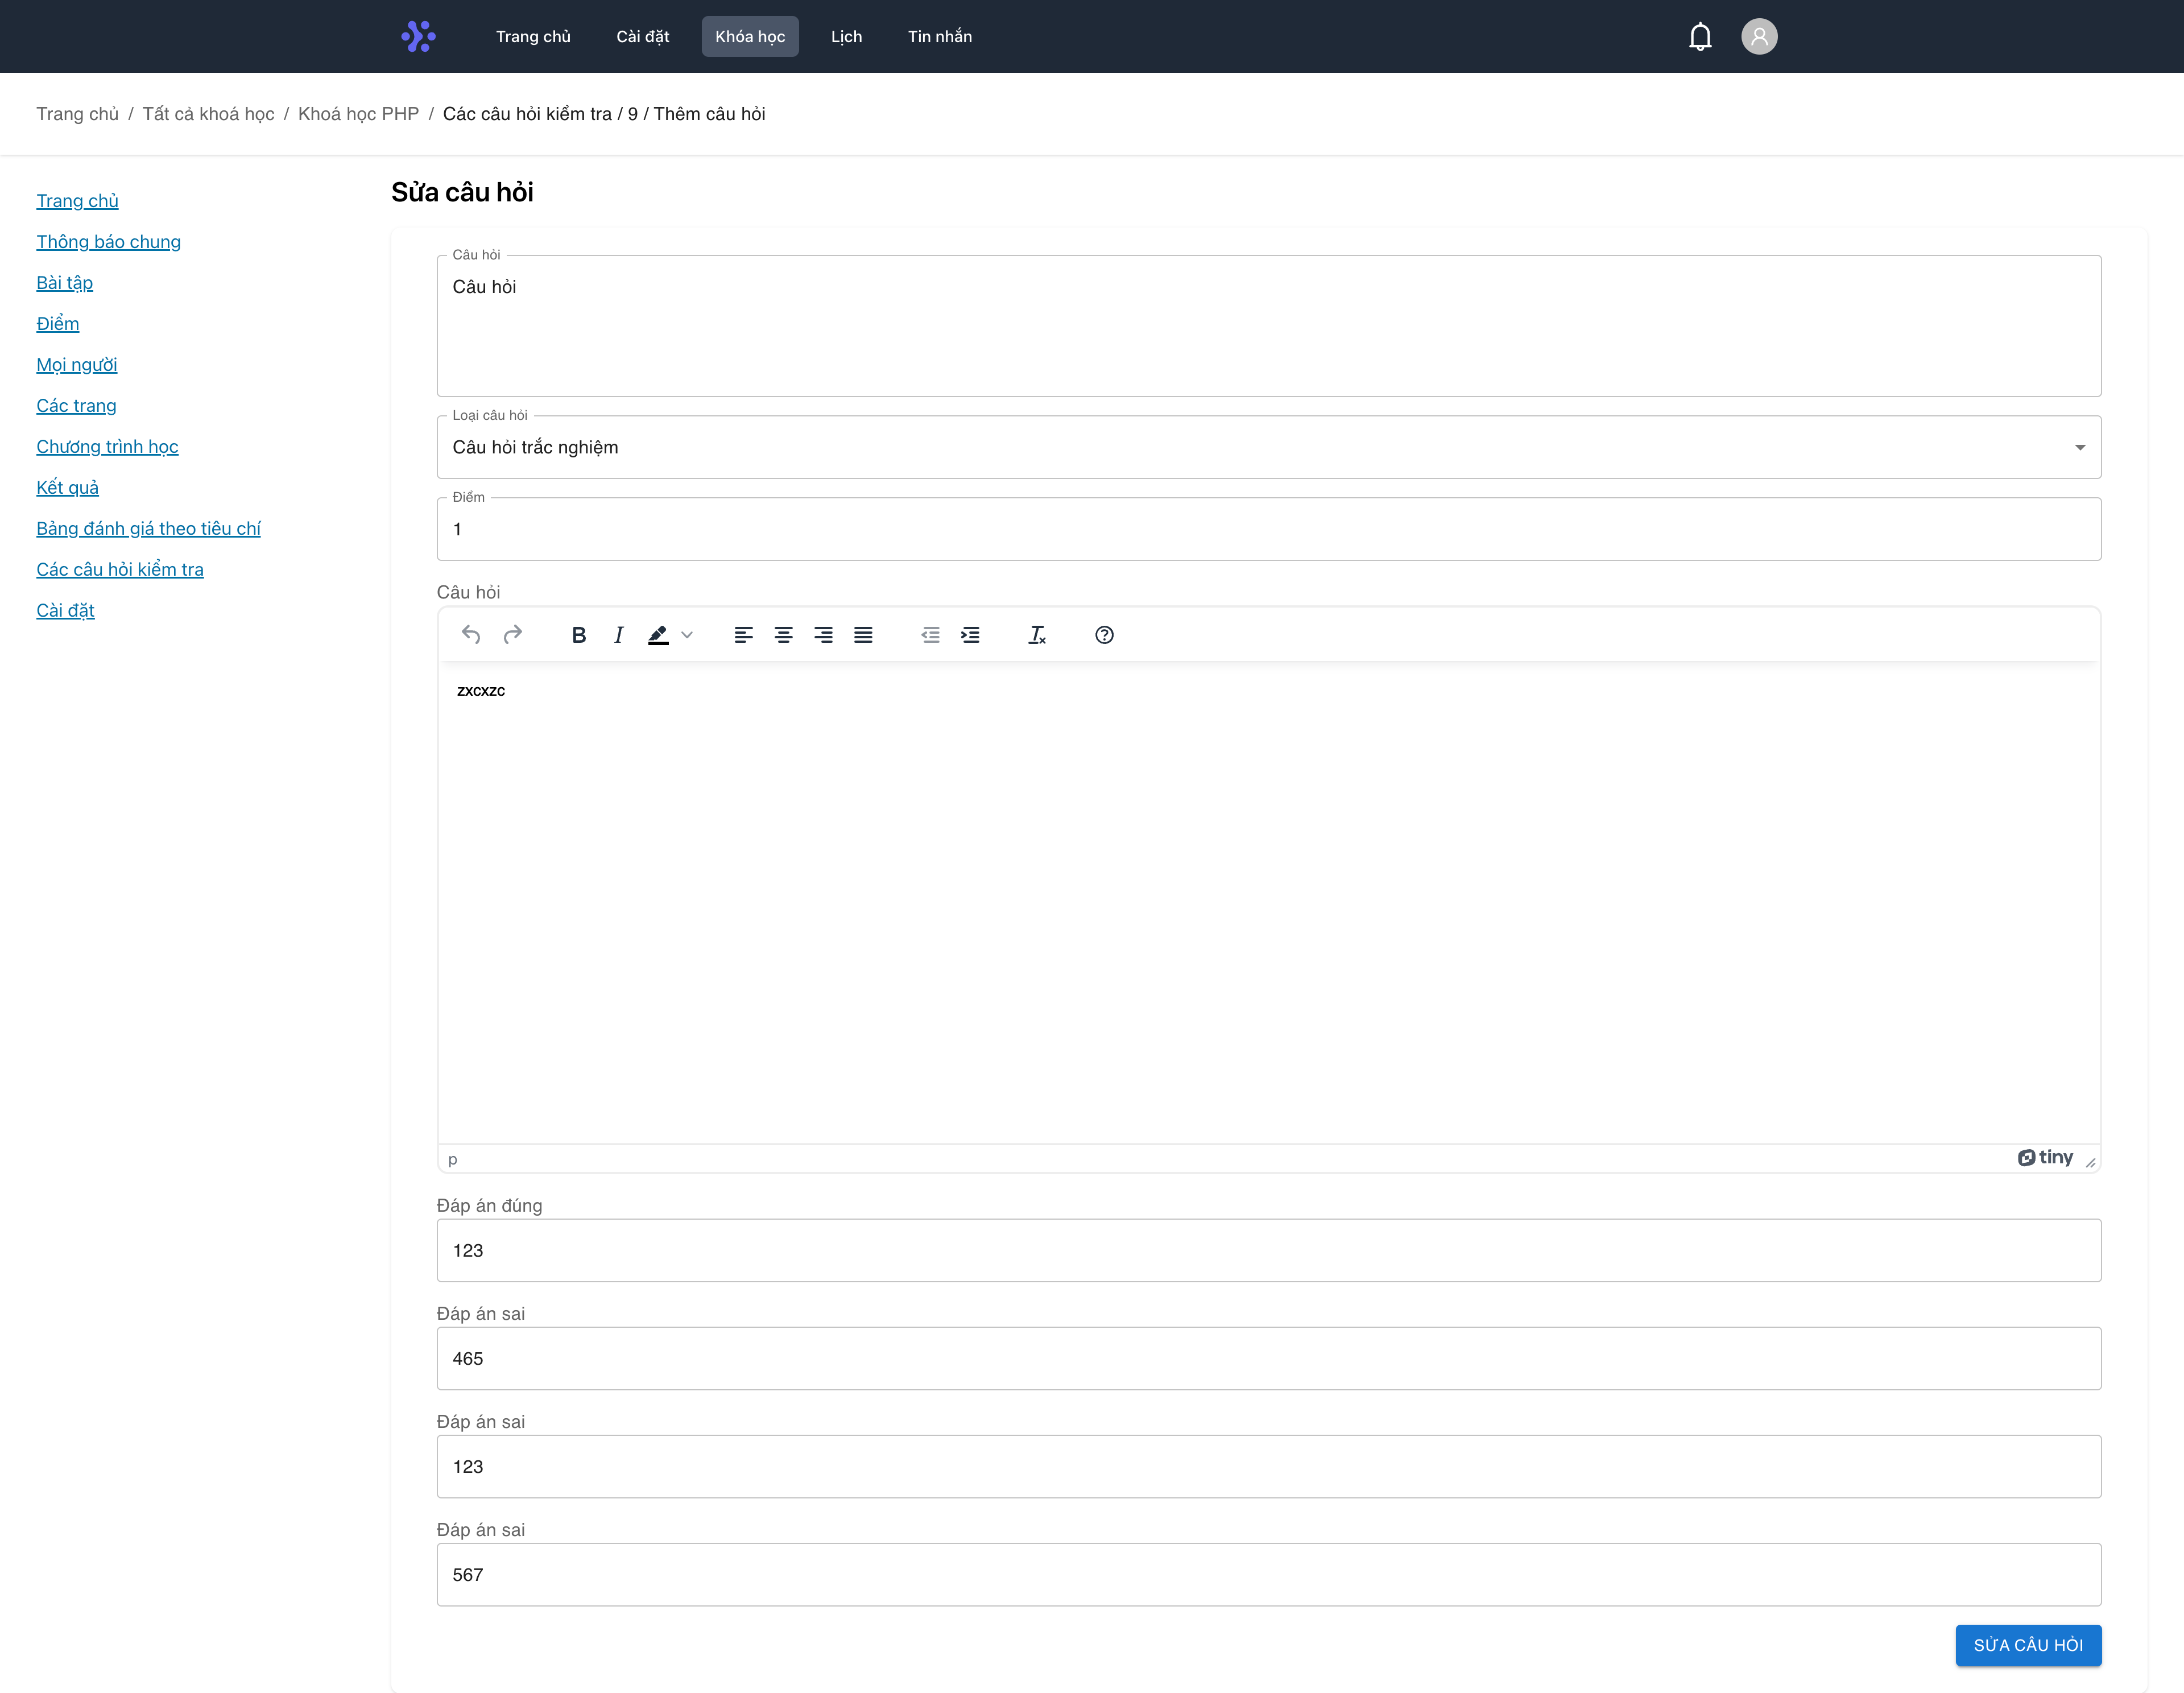
\includegraphics[width=300pt, height=200pt]{chinh-sua-cau-hoi-trong-cau-hoi-kiem-tra}
                    \caption{Màn hình chỉnh sửa câu hỏi trong câu hỏi kiểm tra của phần quản trị viên}
                    \label{fig:chinh-sua-cau-hoi-trong-cau-hoi-kiem-tra}
                \end{figure}
                \FloatBarrier

                \item Phần lịch sử của phần quản trị viên được thể hiện ở hình \ref{fig:lich-su}:
                \begin{figure}[hbt!]
                    \centering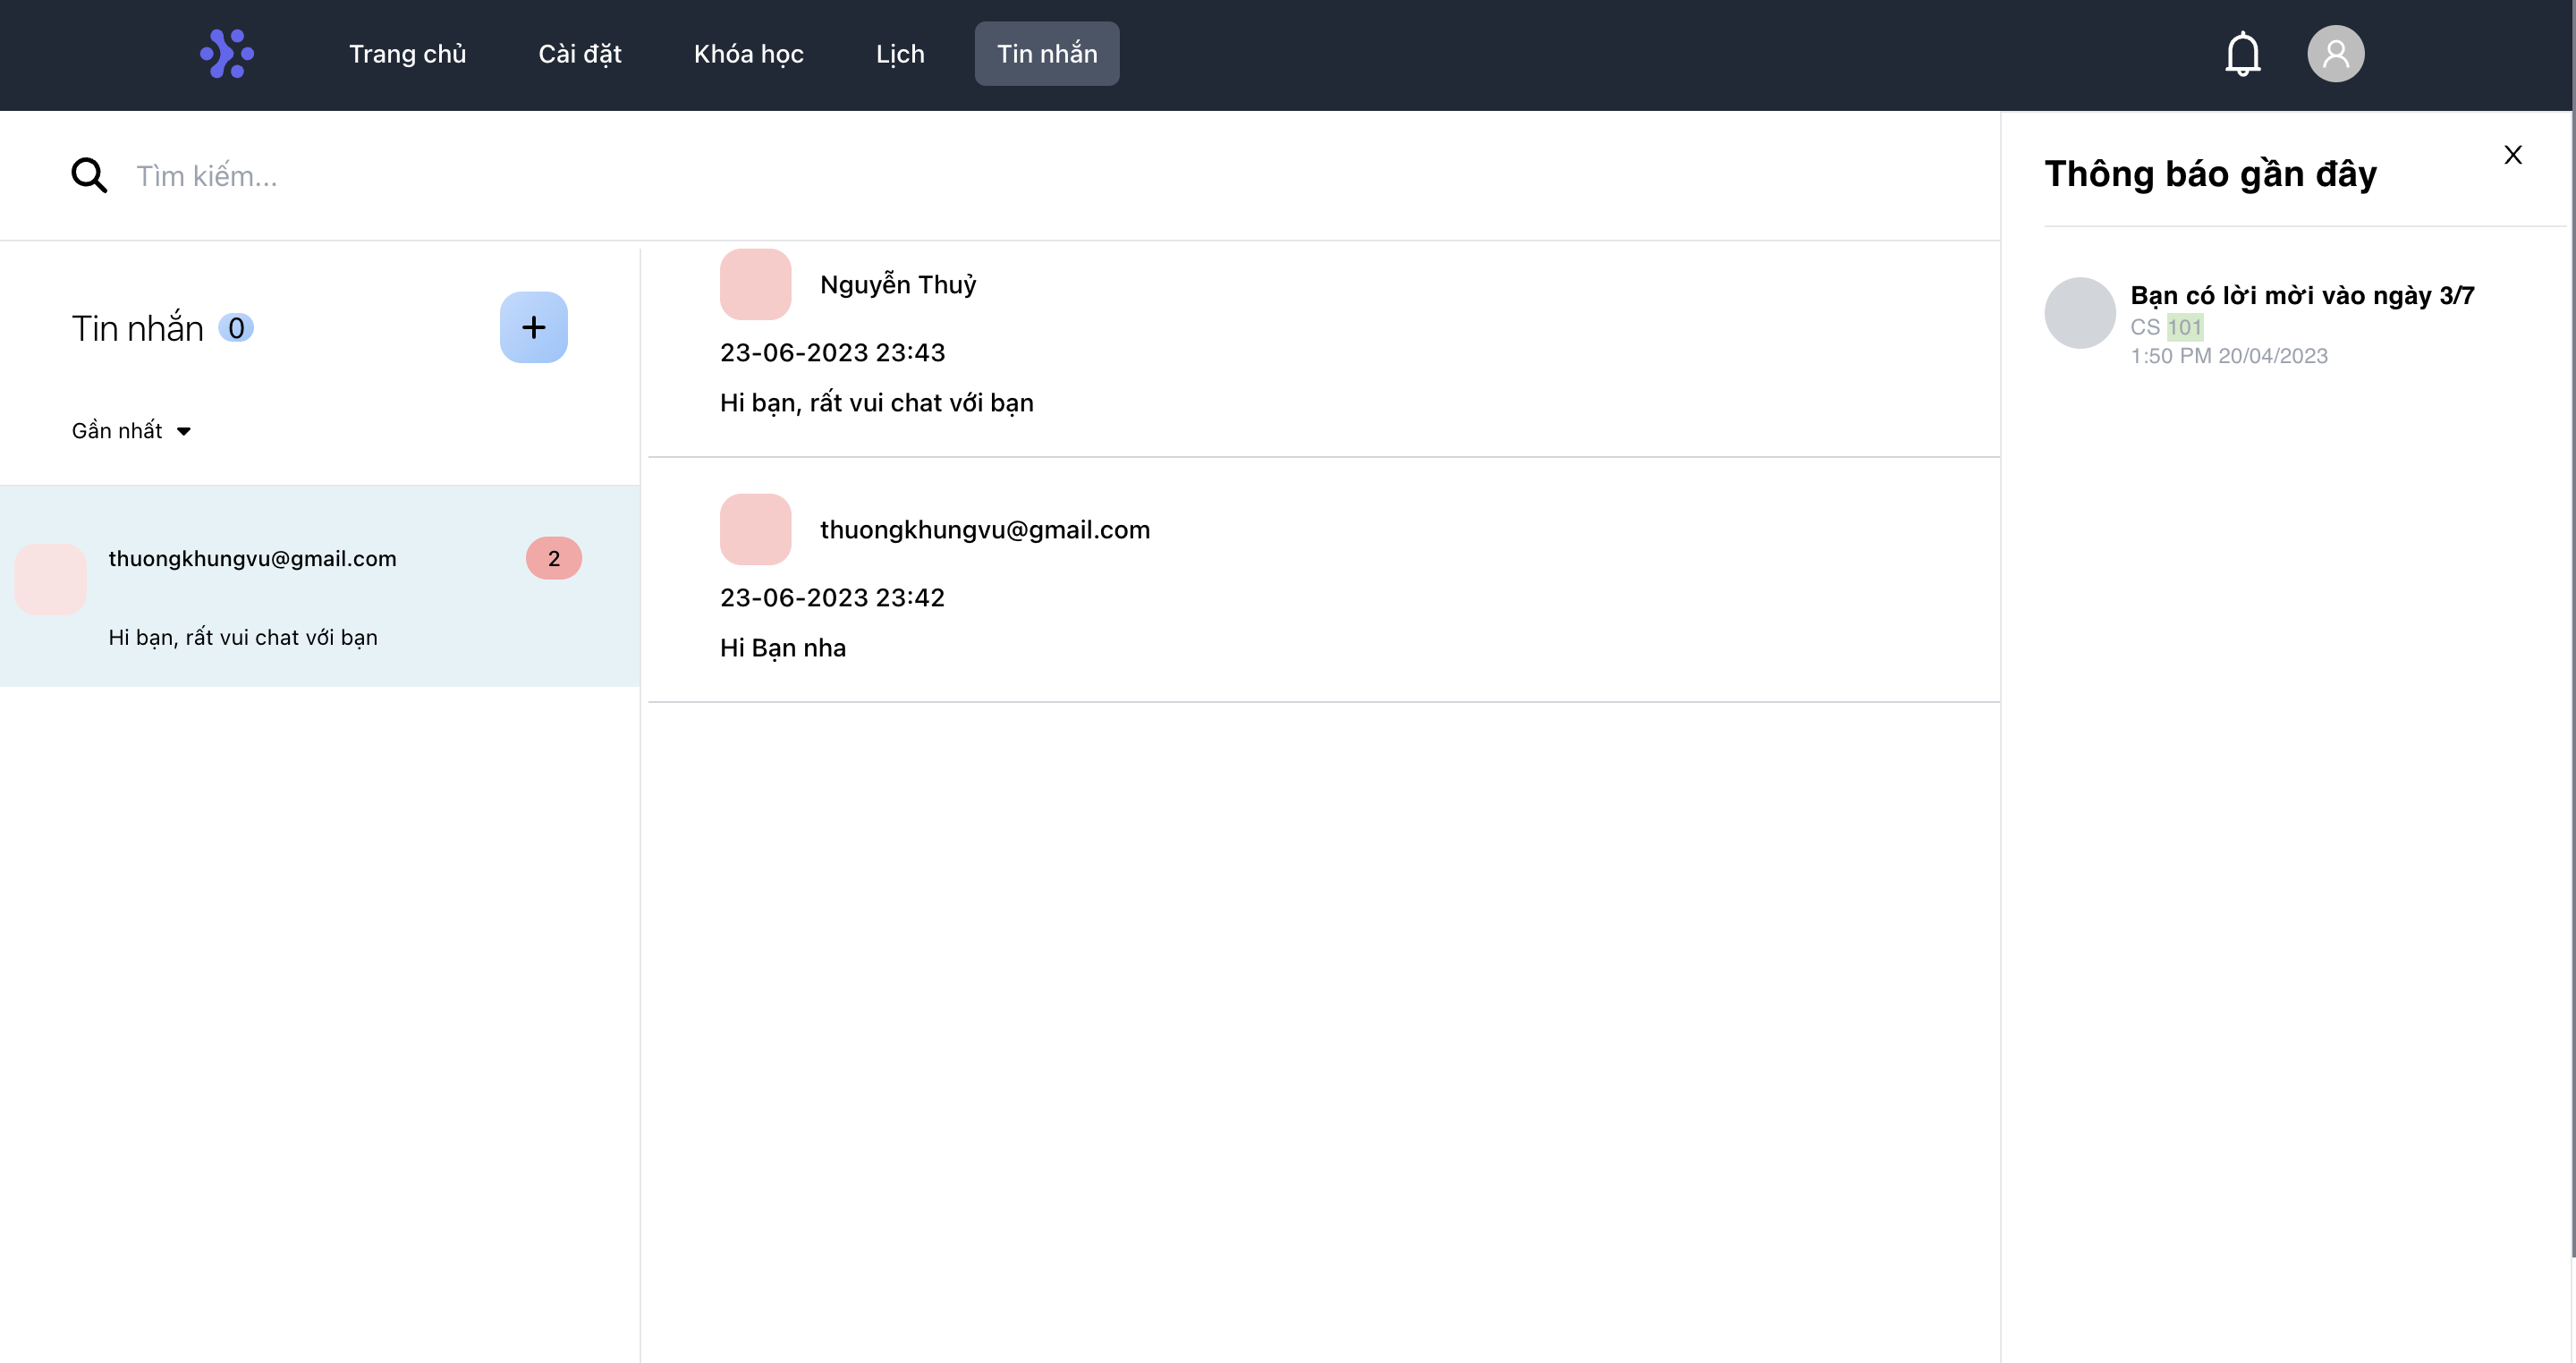
\includegraphics[width=300pt, height=200pt]{lich-su}
                    \caption{Màn hình lịch sử của phần quản trị viên}
                    \label{fig:lich-su}
                \end{figure}
                \FloatBarrier

                \item Phần sự kiện của phần quản trị viên được thể hiện ở hình \ref{fig:su-kien}:
                \begin{figure}[hbt!]
                    \centering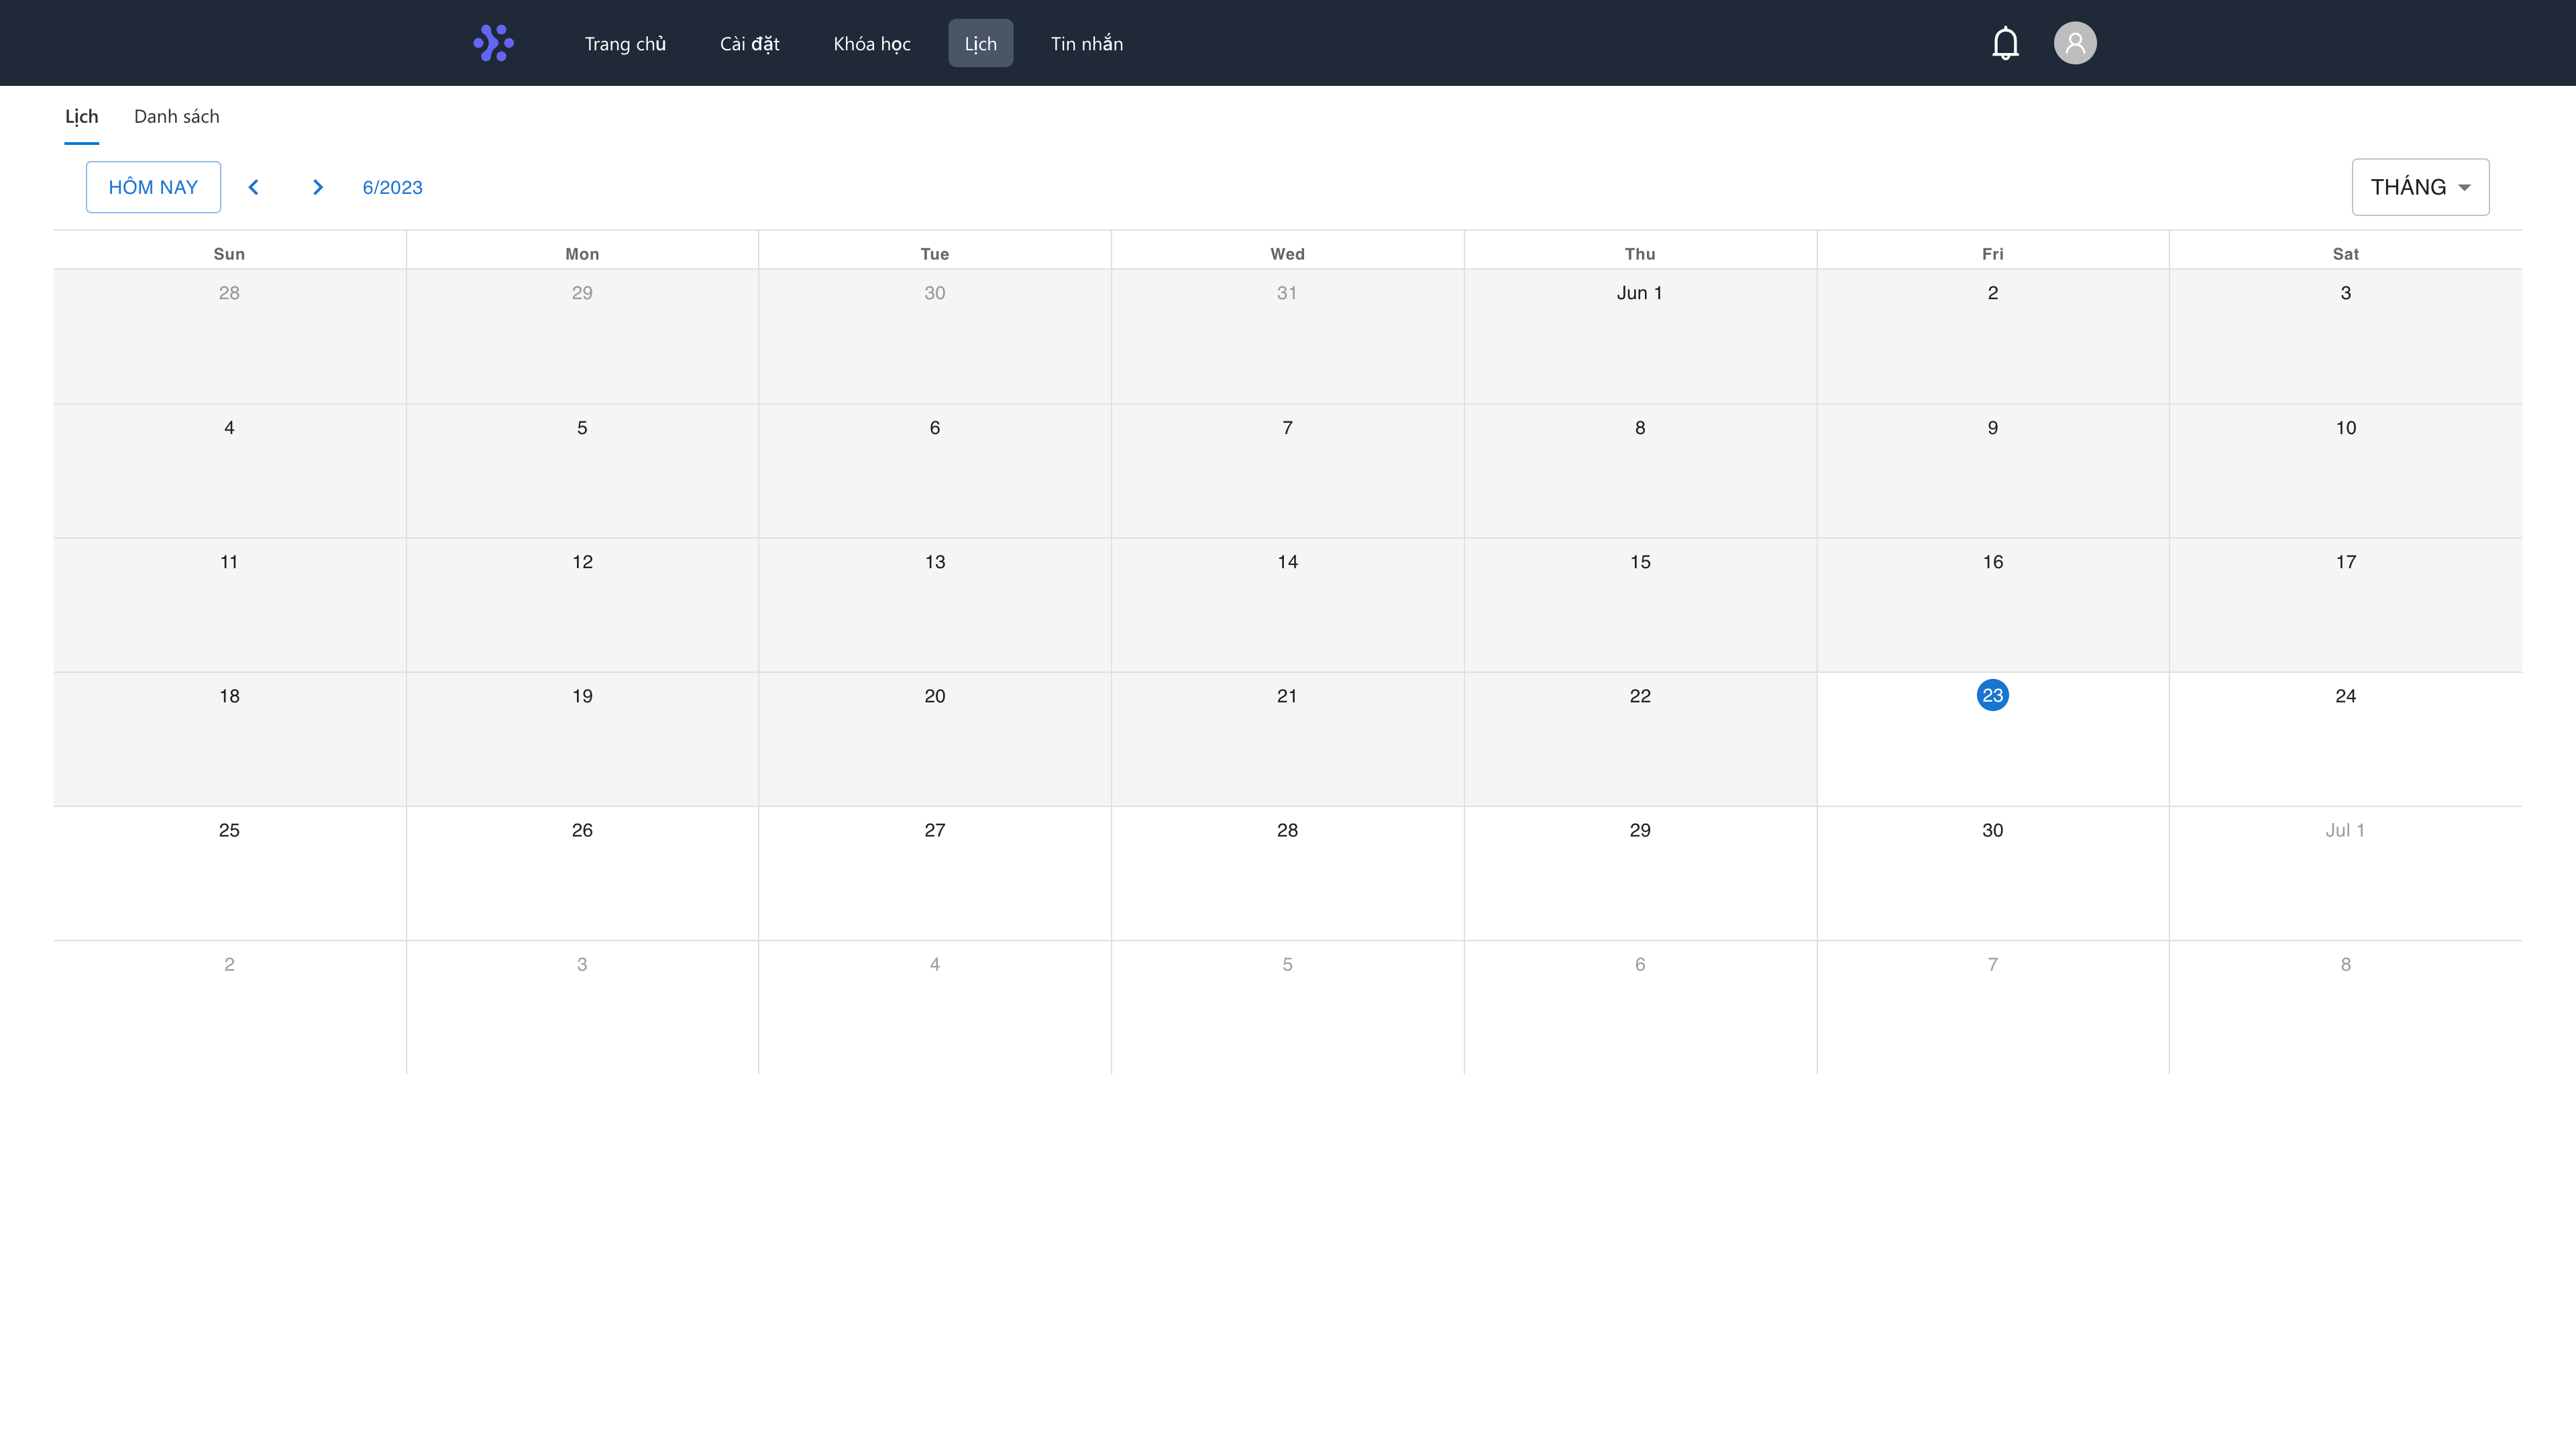
\includegraphics[width=300pt, height=200pt]{su-kien}
                    \caption{Màn hình sự kiện của phần quản trị viên}
                    \label{fig:su-kien}
                \end{figure}
                \FloatBarrier

                \item Phần danh sách sự kiện của phần quản trị viên được thể hiện ở hình \ref{fig:danh-sach-su-kien}:
                \begin{figure}[hbt!]
                    \centering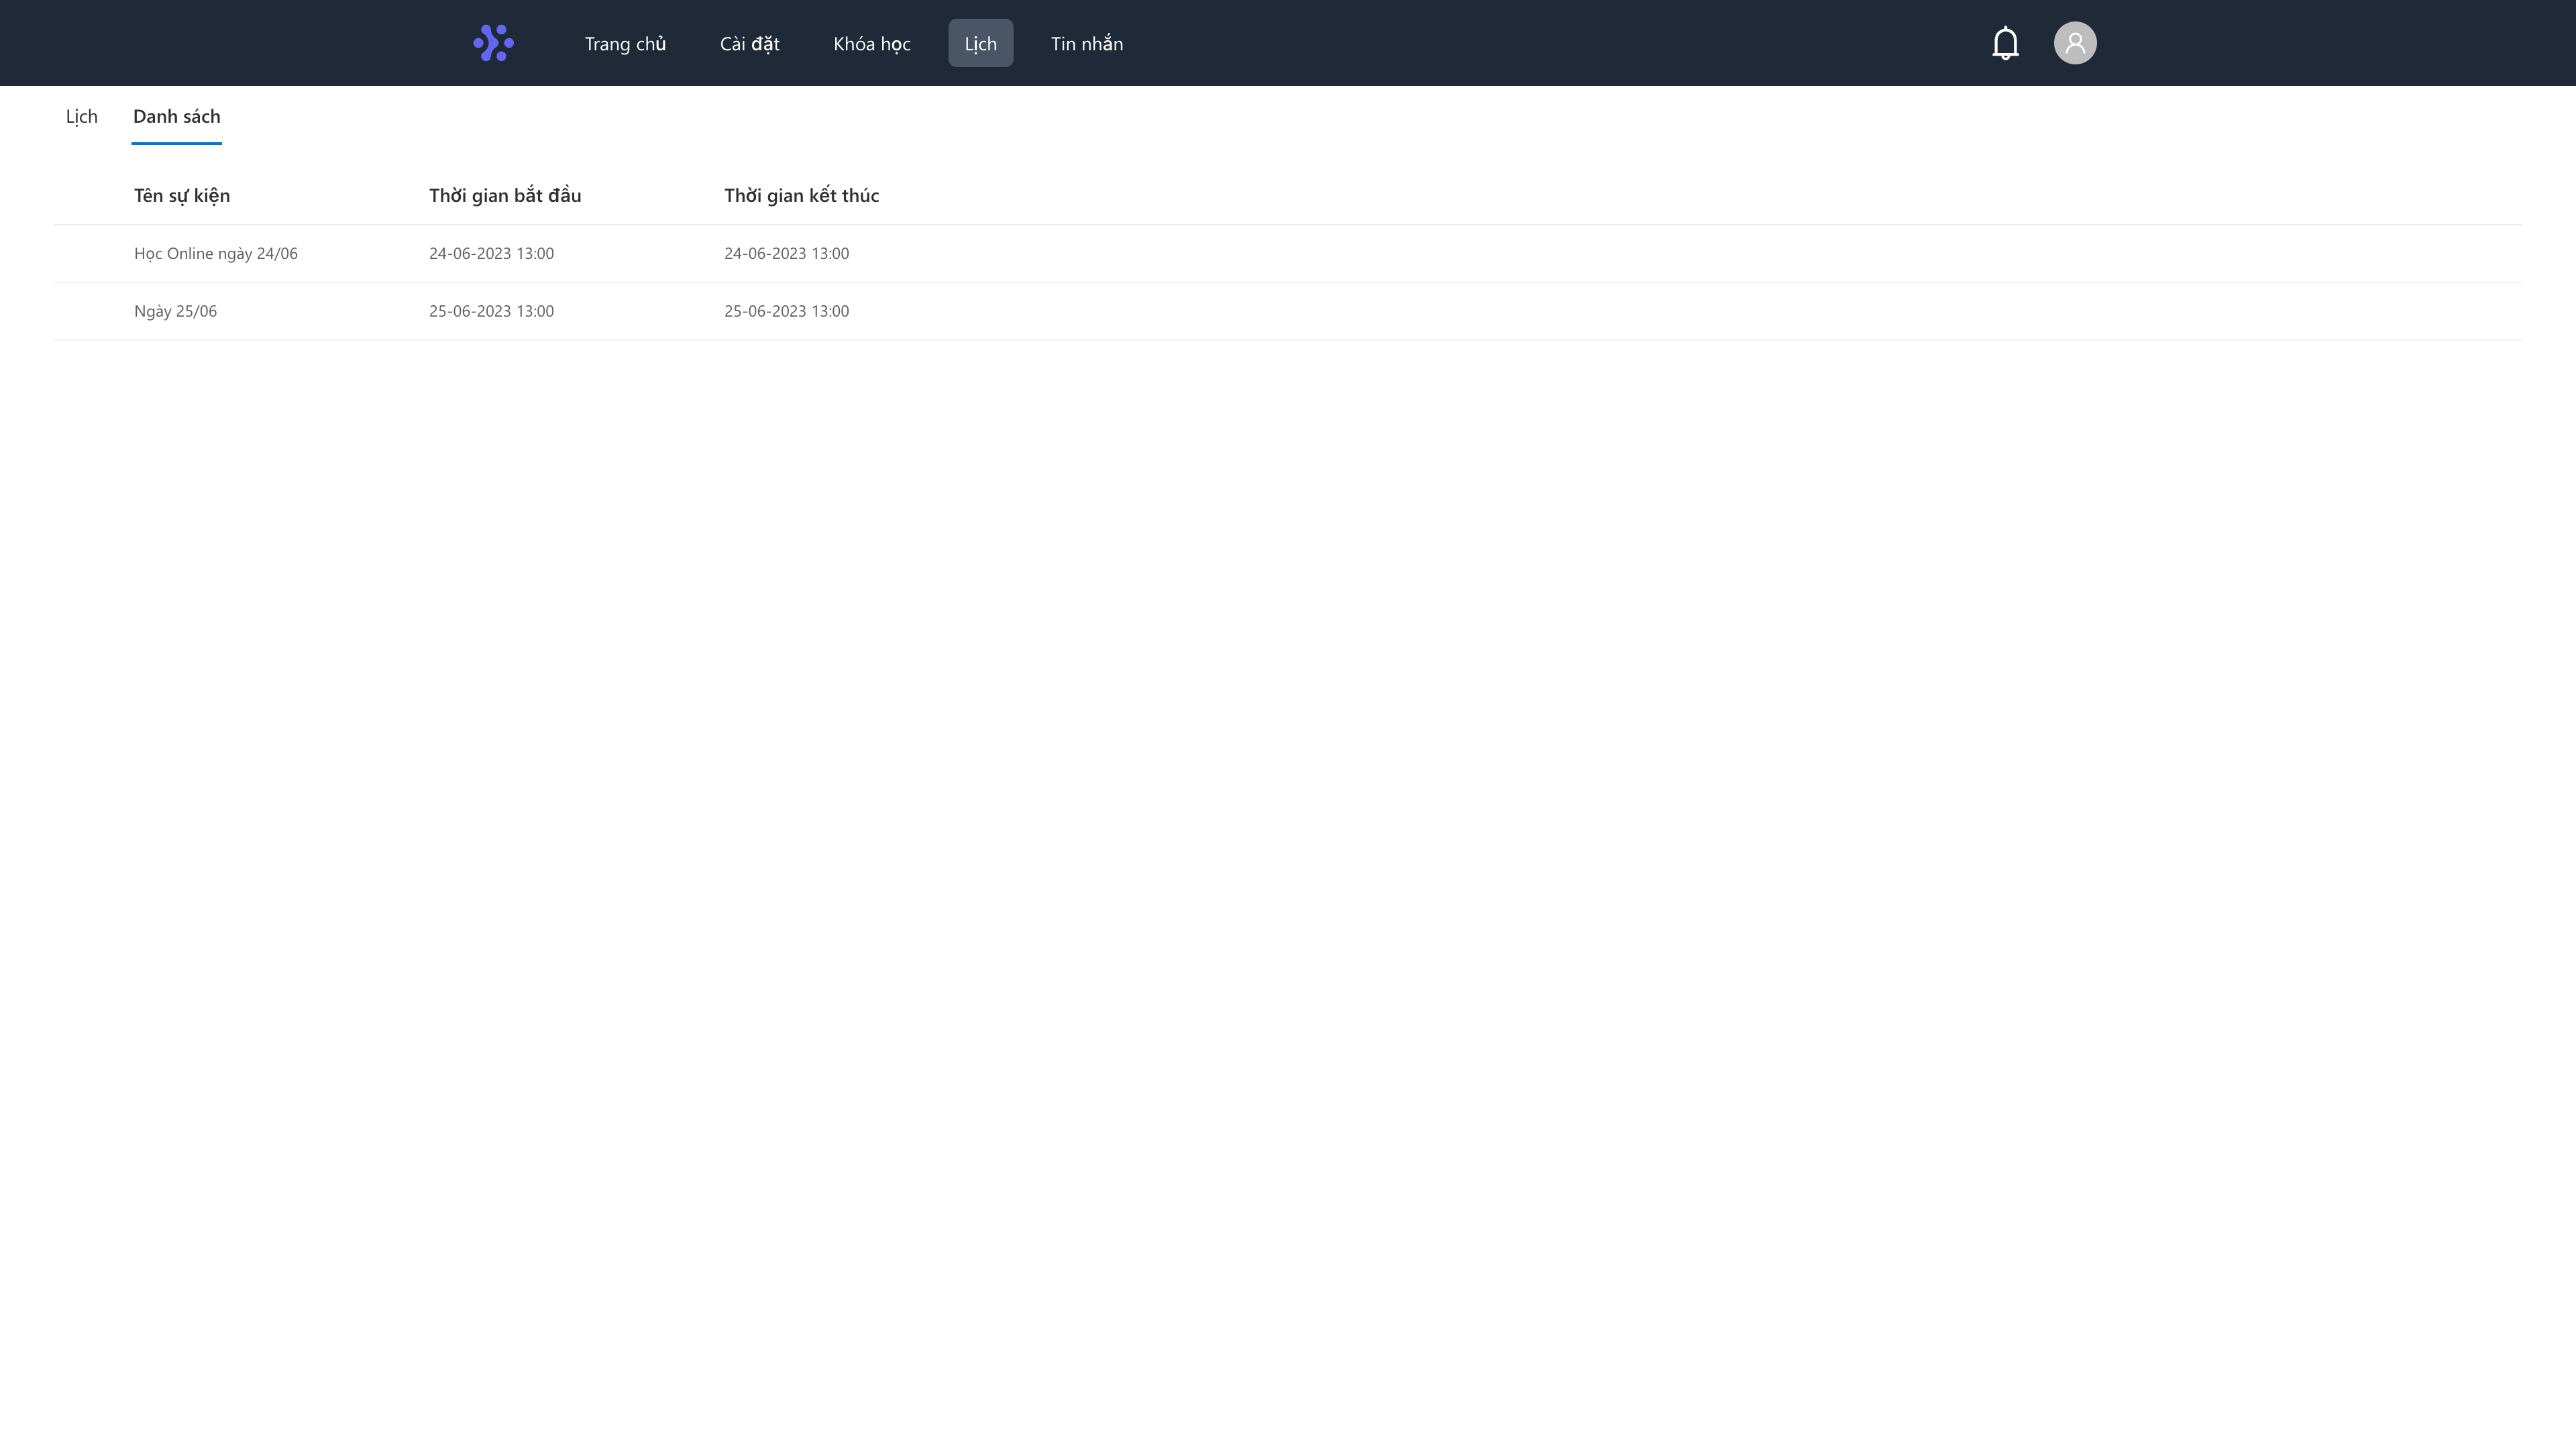
\includegraphics[width=300pt, height=200pt]{danh-sach-su-kien}
                    \caption{Màn hình danh sách sự kiện của phần quản trị viên}
                    \label{fig:danh-sach-su-kien}
                \end{figure}
                \FloatBarrier

                \item Phần tạo sự kiện của phần quản trị viên được thể hiện ở hình \ref{fig:tao-su-kien}:
                \begin{figure}[hbt!]
                    \centering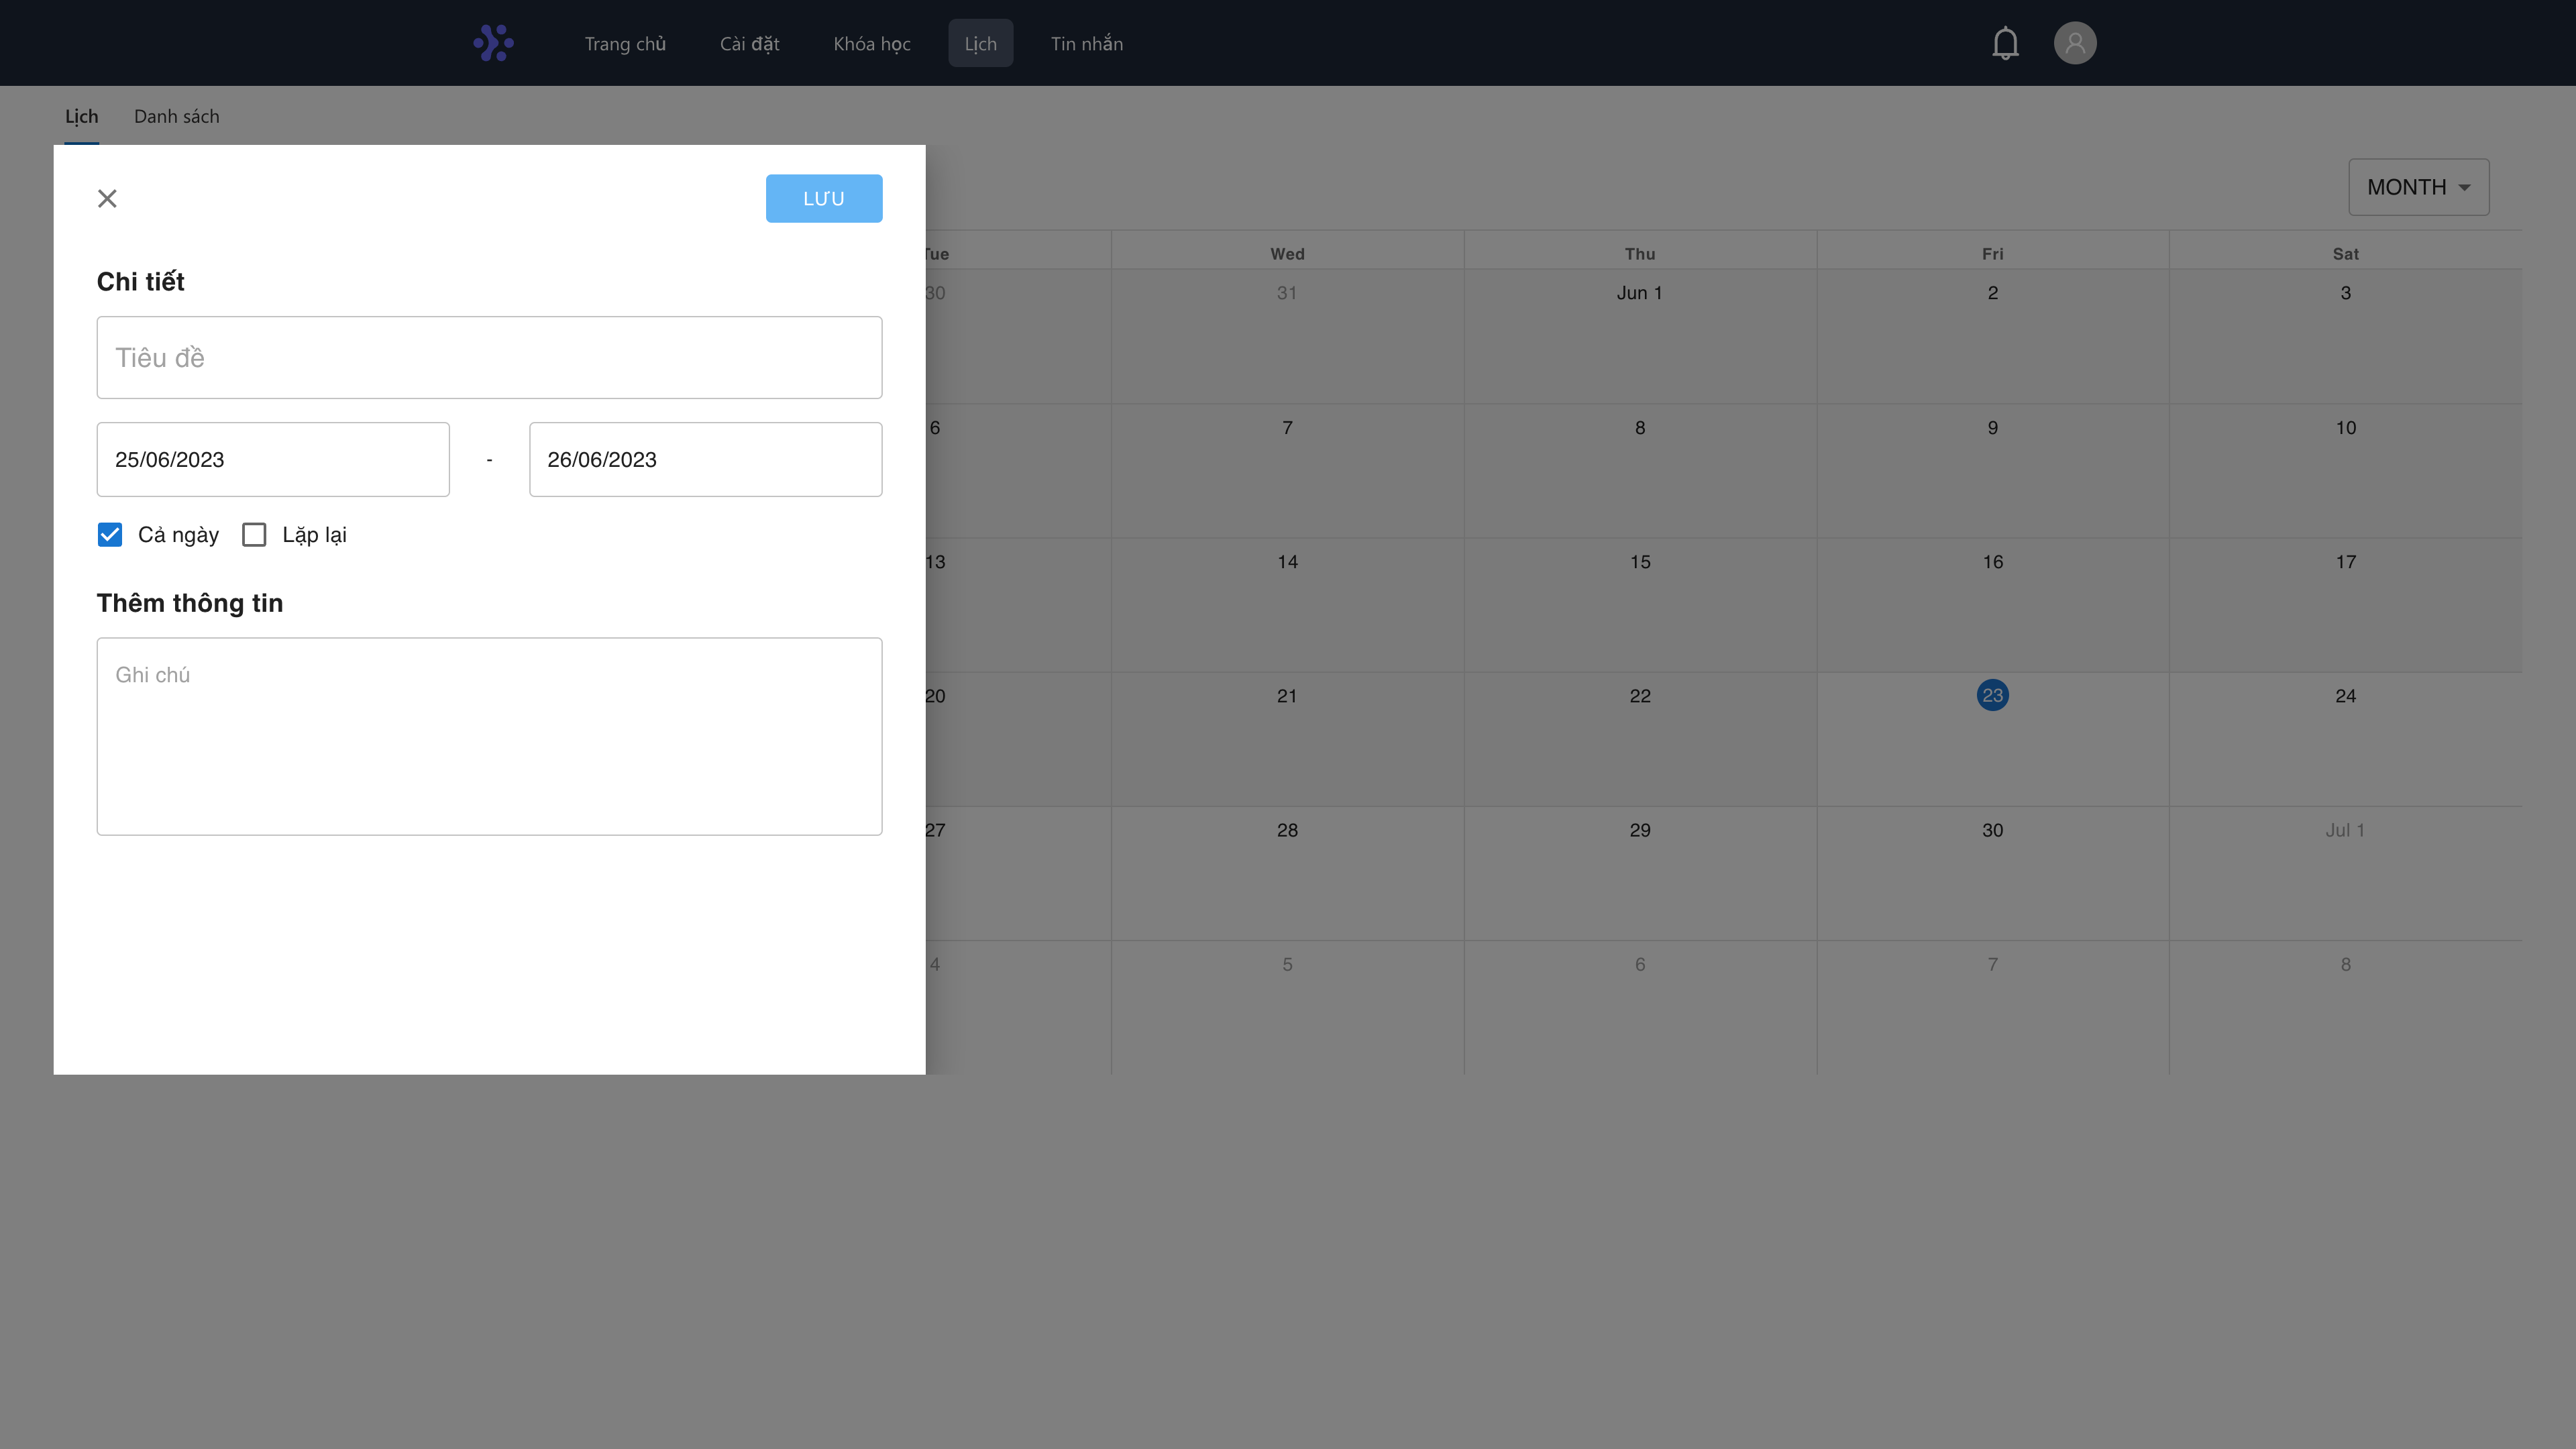
\includegraphics[width=300pt, height=200pt]{tao-su-kien}
                    \caption{Màn hình tạo sự kiện của phần quản trị viên}
                    \label{fig:tao-su-kien}
                \end{figure}
                \FloatBarrier

                \item Phần tin nhắn của phần quản trị viên được thể hiện ở hình \ref{fig:tin-nhan}:
                \begin{figure}[hbt!]
                    \centering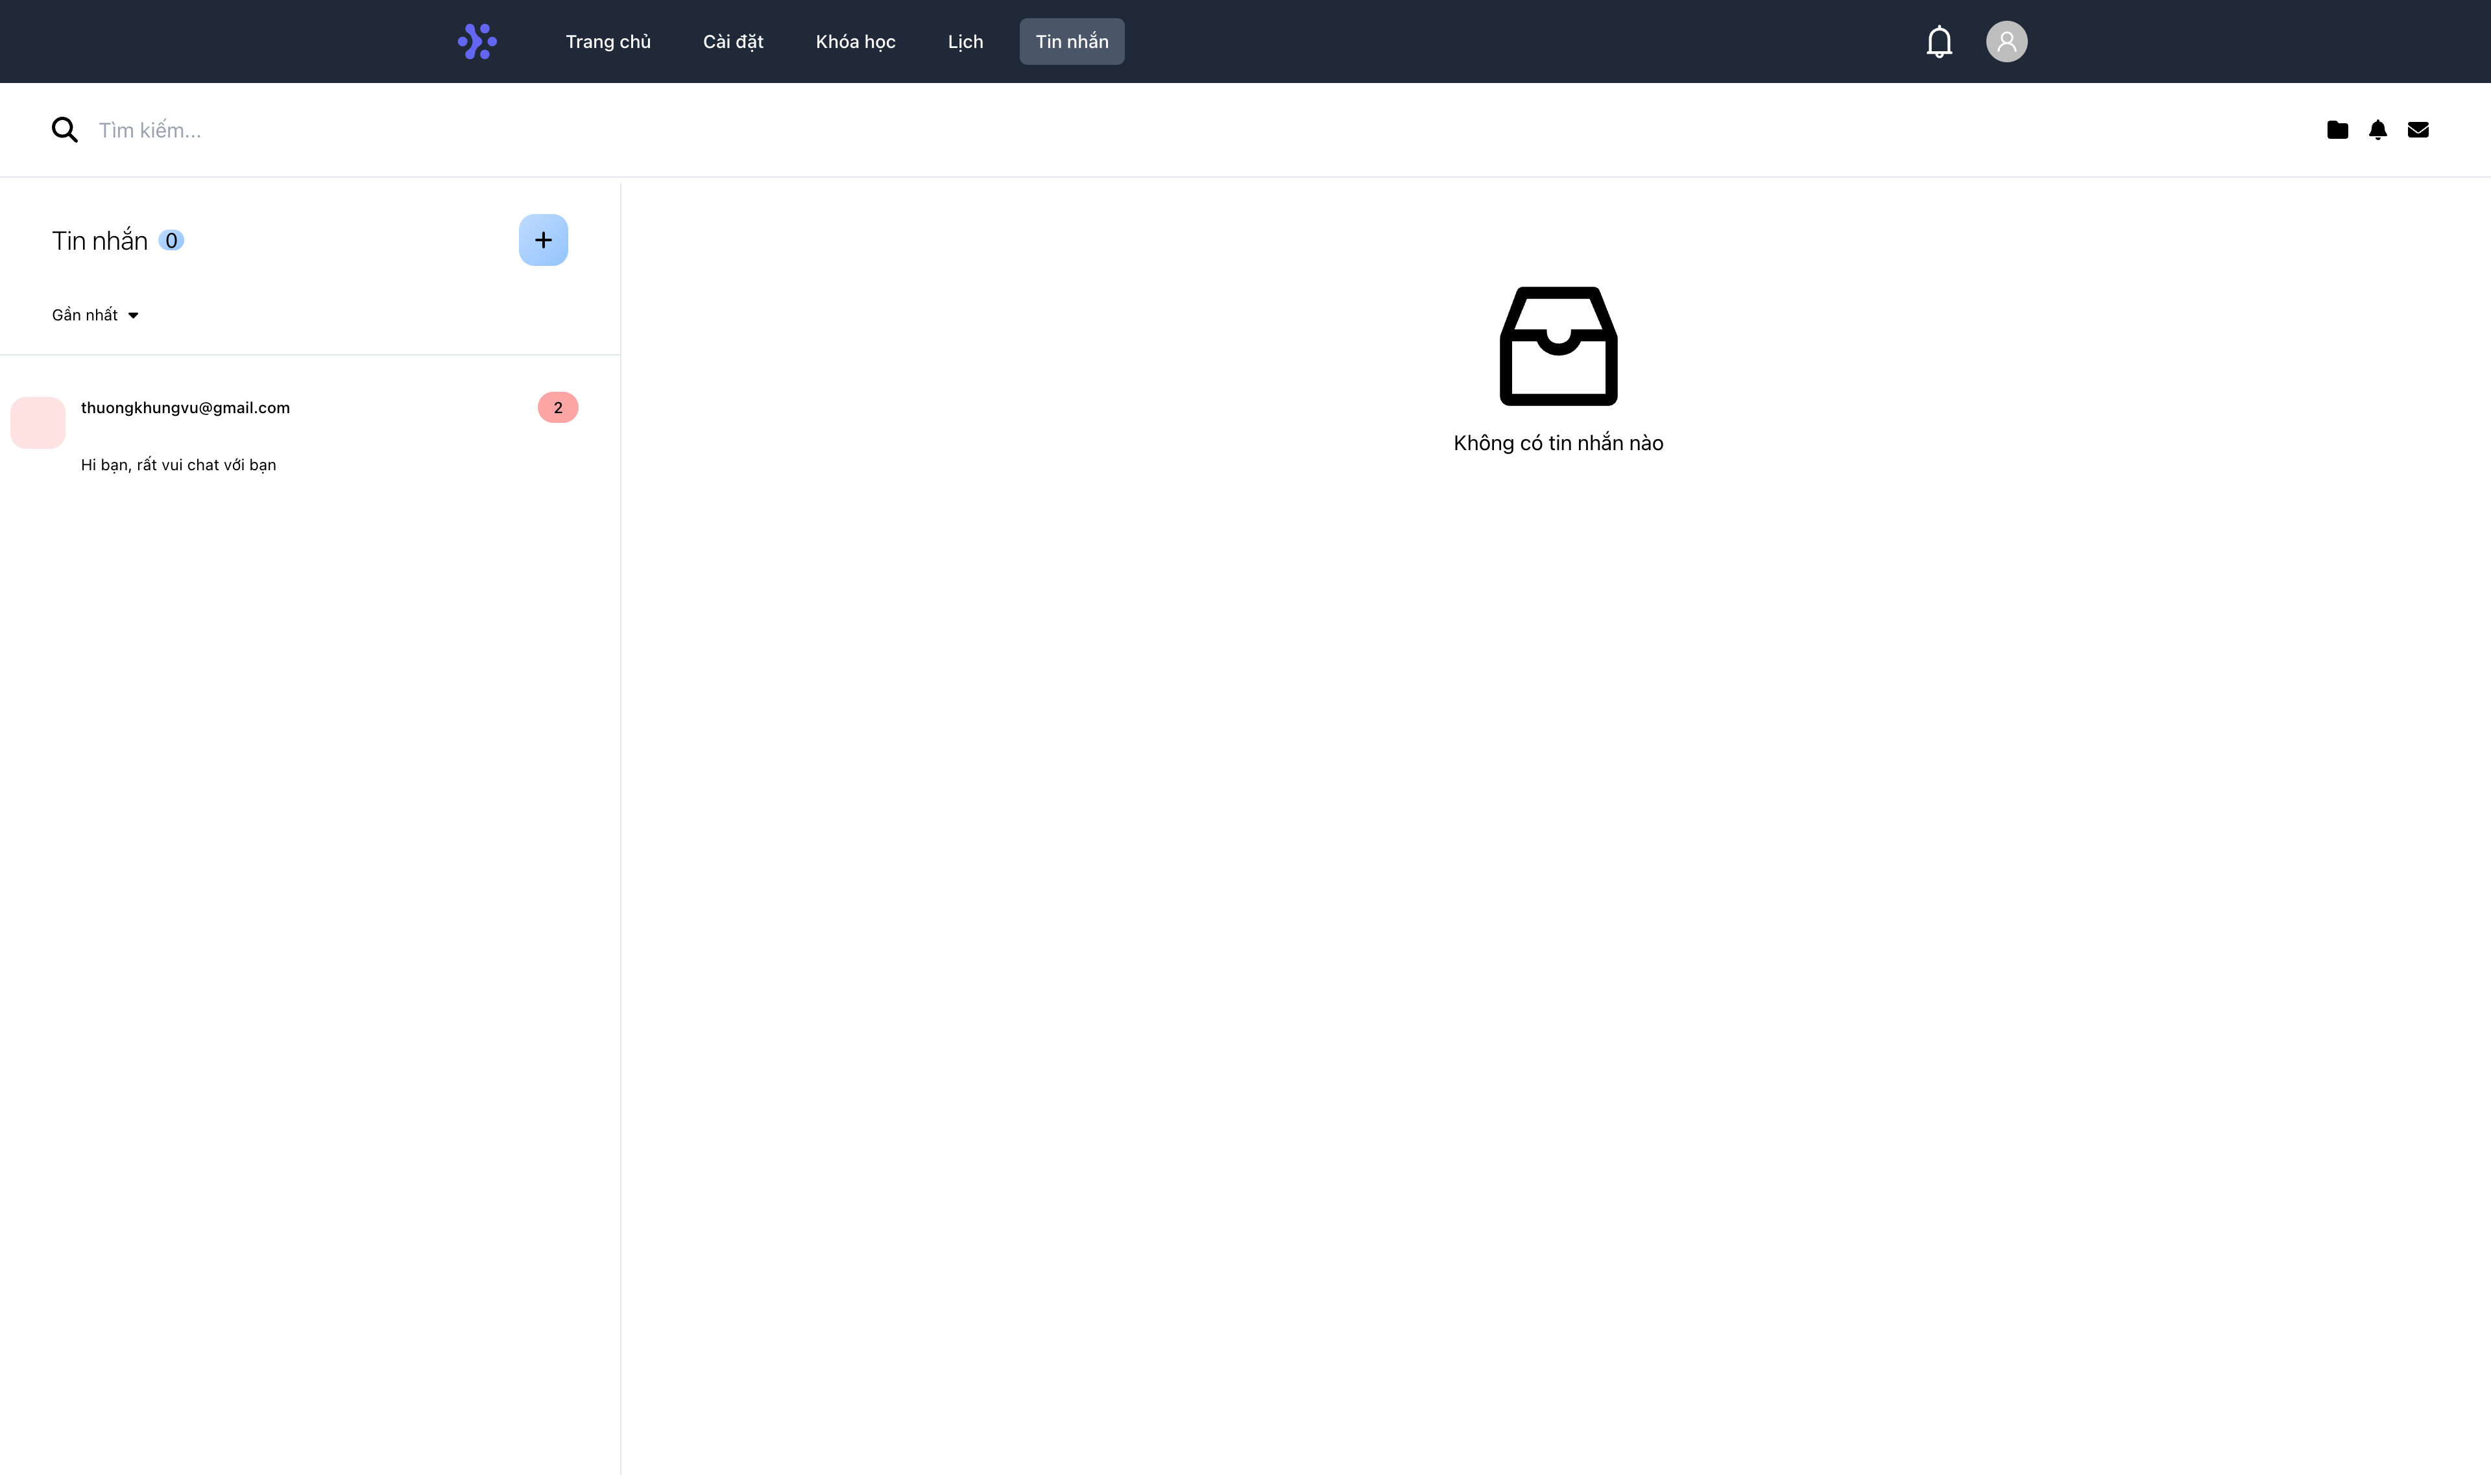
\includegraphics[width=300pt, height=200pt]{tin-nhan}
                    \caption{Màn hình tin nhắn của phần quản trị viên}
                    \label{fig:tin-nhan}
                \end{figure}
                \FloatBarrier

                \item Phần chi tiết tin nhắn của phần quản trị viên được thể hiện ở hình \ref{fig:chi-tiet-tin-nhan}:
                \begin{figure}[hbt!]
                    \centering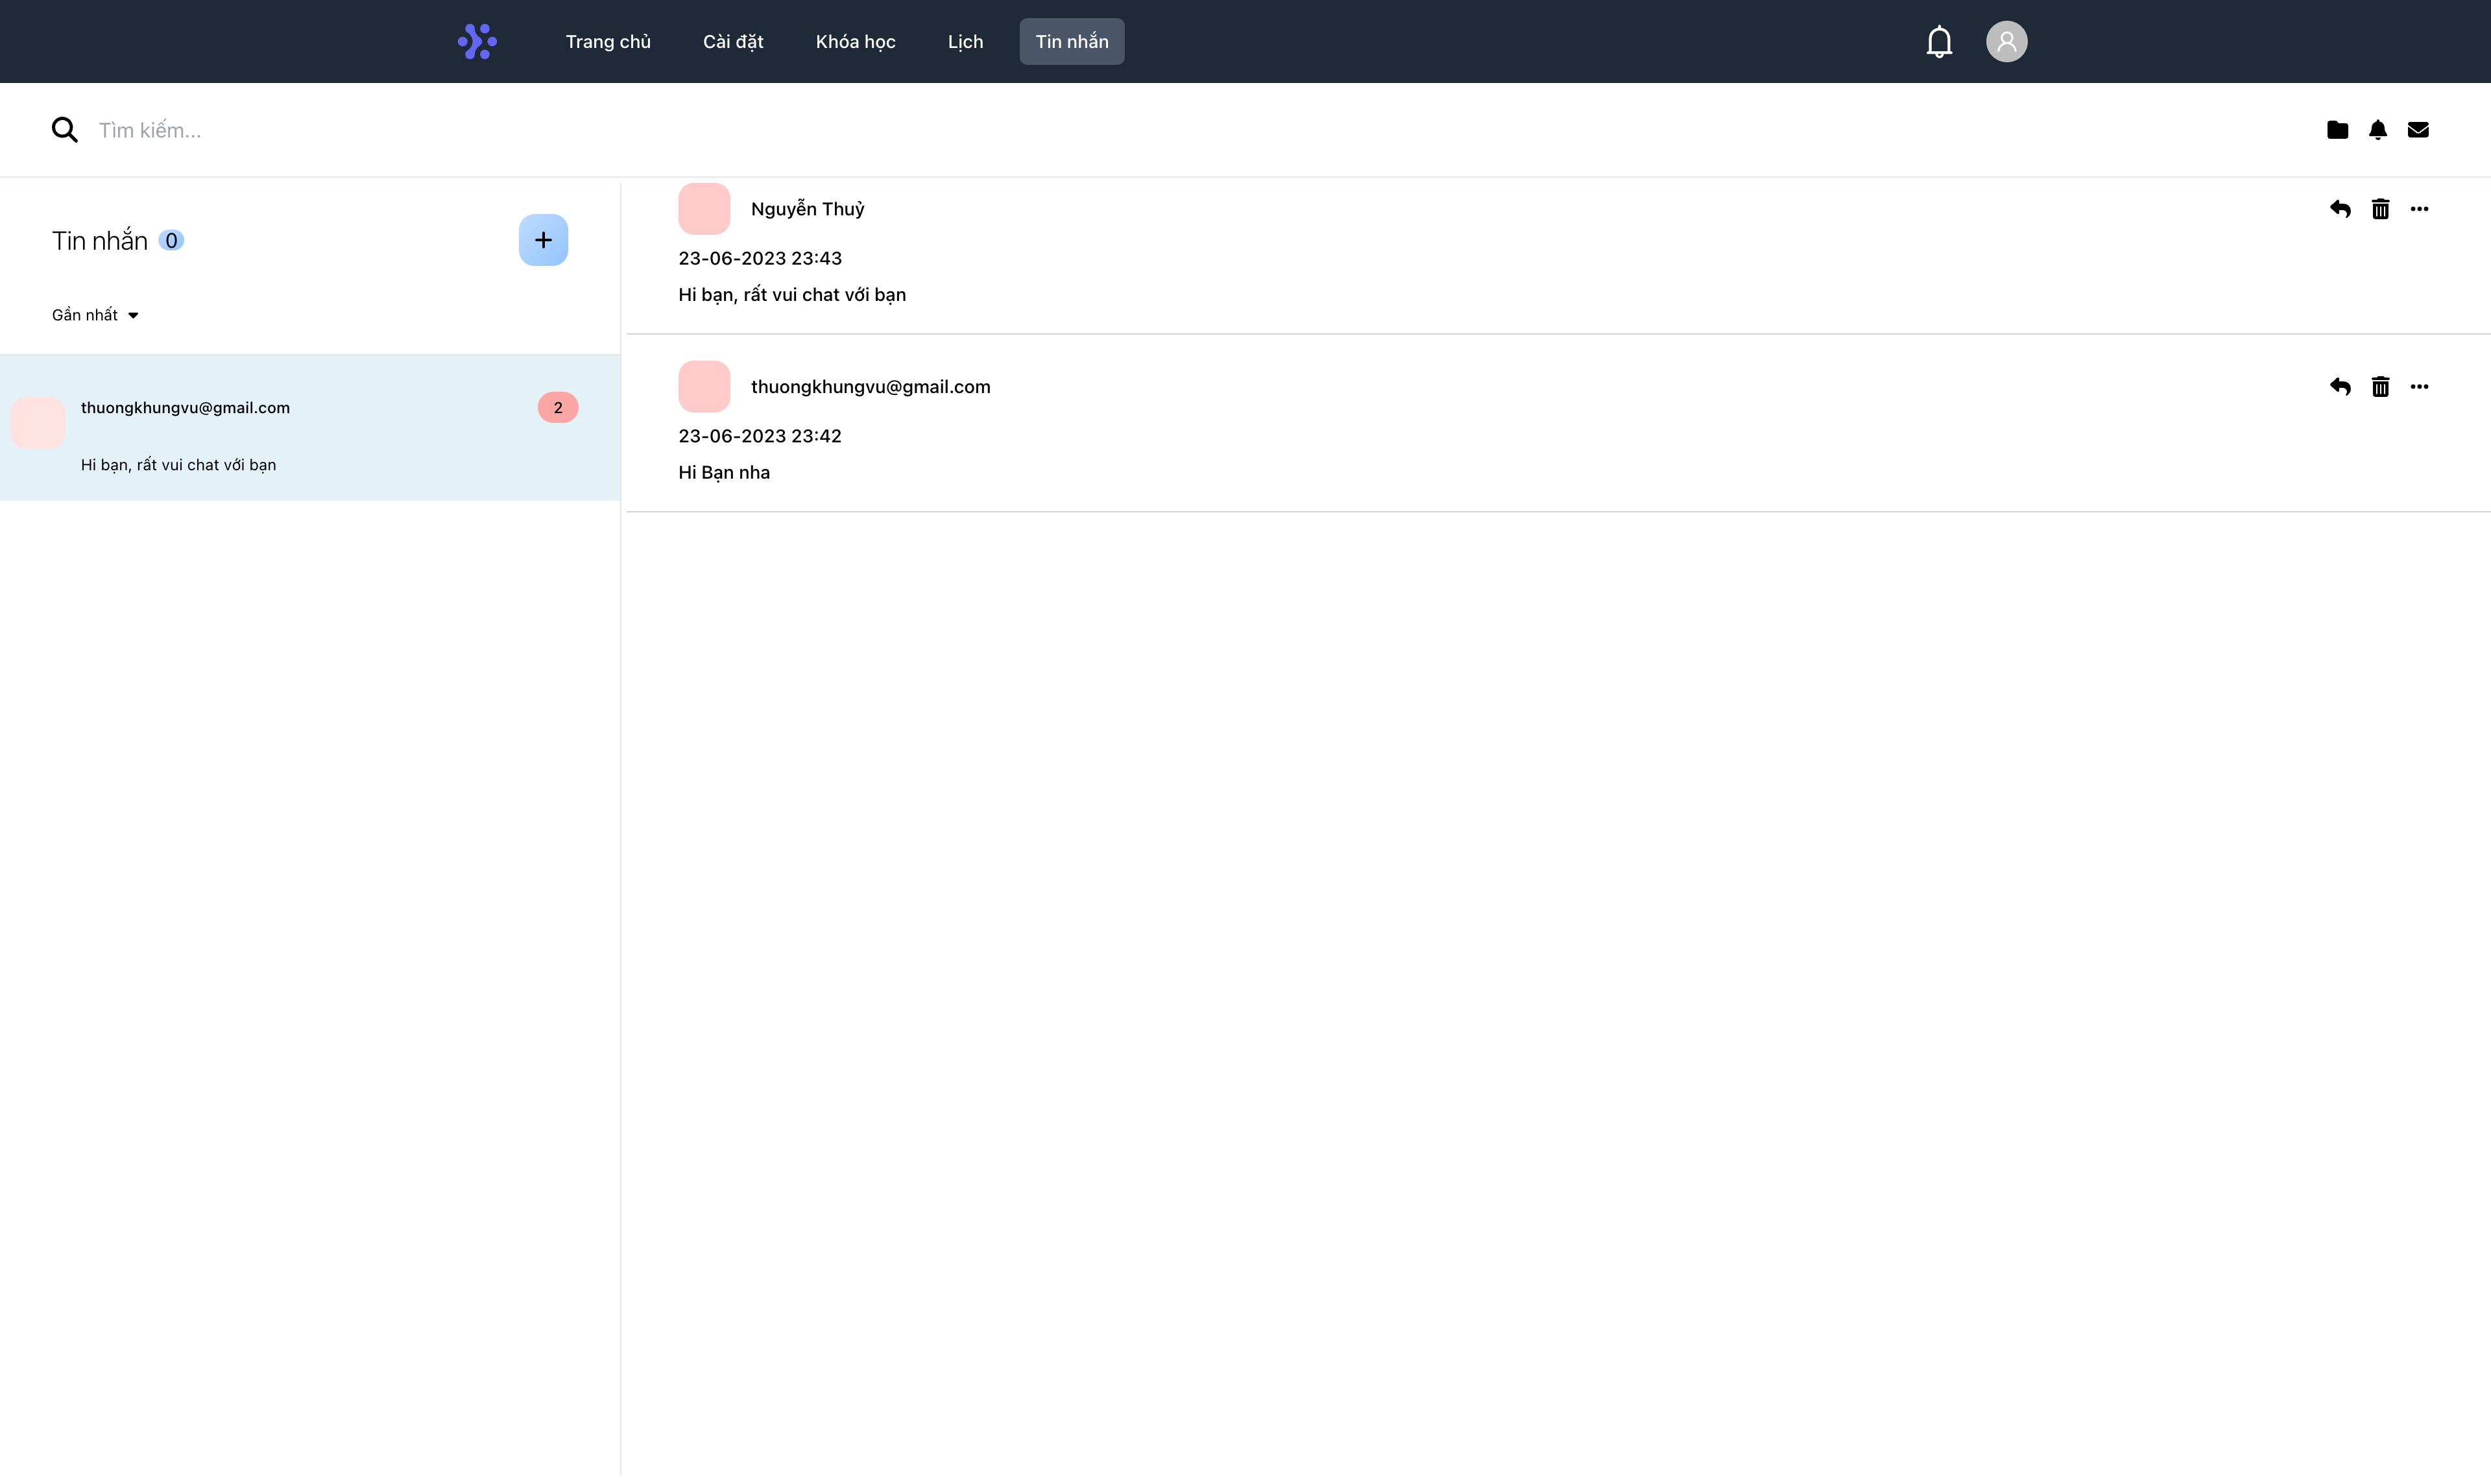
\includegraphics[width=300pt, height=200pt]{chi-tiet-tin-nhan}
                    \caption{Màn hình chi tiết tin nhắn của phần quản trị viên}
                    \label{fig:chi-tiet-tin-nhan}
                \end{figure}
                \FloatBarrier
        \end{itemize}

\section{Tài liệu API}
    \subsection{Xác thực và uỷ quyền}
        Canvas LMS sử dụng cơ chế xác thực OAuth2 để xác thực và uỷ quyền người dùng. Để sử dụng API, người dùng cần có một mã truy cập (access token) hợp lệ. Mã truy cập này có thể được lấy bằng cách sử dụng một trong các luồng xác thực OAuth2 được hỗ trợ bởi Canvas LMS. Các luồng xác thực này bao gồm:
        
        Bước 1: Tạo một client id và một secret ở trên Canvas LMS
        
        Bước 2: Sử dụng id để lấy mã code
        
            Trong đó:
            \begin{itemize}
            \item \textbf{client\_id}: id của client được tạo ở bước 1
            \item \textbf{response\_type}: loại phản hồi, ở đây là mã code
            \item \textbf{redirect\_uri}: địa chỉ để nhận mã code
            \end{itemize}

            Response sẽ được trả về theo dạng sau:
            \begin{lstlisting}[language=bash]
            http://localhost:3000/oauth2response?code=1234567890
            \end{lstlisting}

        Bước 3: Sử dụng mã code để lấy mã truy cập
        \begin{lstlisting}[language=bash]
            POST https://35.247.158.82/login/oauth2/token
        \end{lstlisting}
        \begin{itemize}
            \item \textbf{grant\_type}: loại phân quyền, ở đây là mã authorization\_code
            \item \textbf{client\_id}: id của client được tạo ở bước 1
            \item \textbf{client\_secret}: secret của client được tạo ở bước 1
            \item \textbf{code}: mã code được lấy ở bước 2
        \end{itemize}

        Response sẽ được trả về theo dạng sau:
        \begin{lstlisting}[language=bash]
            {
            "access_token": "1234567890",
            "token_type": "Bearer",
            "user": {
                "id": 1,
                "name": "John Doe",
                "global_id": "1234567890",
                "avatar_url": "http://localhost:3000/images/users/0001-1234567890/avatar.png"
            }
            }
        \end{lstlisting}

\subsection{Khoá học}

            Một object khoá học sẽ có dạng: 
            \begin{lstlisting}[language=bash]
            {
                "id": 370663,
                "sis_course_id": null,
                "uuid": "WvAHhY5FINzq5IyRIJybGeiXyFkG3SqHUPb7jZY5",
                "integration_id": null,
                "sis_import_id": 34,
                "name": "InstructureCon 2012",
                "course_code": "INSTCON12",
                "original_name": "InstructureCon-2012-01",
                "workflow_state": "available",
                "account_id": 81259,
                "root_account_id": 81259,
                "enrollment_term_id": 34,
                "grading_periods": null,
                "grading_standard_id": 25,
                "grade_passback_setting": "nightly_sync",
                "created_at": "2012-05-01T00:00:00-06:00",
                "start_at": "2012-06-01T00:00:00-06:00",
                "end_at": "2012-09-01T00:00:00-06:00",
                "locale": "en",
                "total_students": 32,
                "calendar": null,
                "default_view": "feed",
                "syllabus_body": "<p>syllabus html goes here</p>",
                "needs_grading_count": 17,
                "term": null,
                "course_progress": null,
                "apply_assignment_group_weights": true,
                "permissions": "create_discussion_topic":true,"create_announcement":true,
                "is_public": true,
                "is_public_to_auth_users": true,
                "public_syllabus": true,
                "public_syllabus_to_auth": true,
                "public_description": "Come one, come all to InstructureCon 2012!",
                "storage_quota_mb": 5,
                "storage_quota_used_mb": 5,
                "hide_final_grades": false,
                "license": "Creative Commons",
                "allow_student_assignment_edits": false,
                "allow_wiki_comments": false,
                "allow_student_forum_attachments": false,
                "open_enrollment": true,
                "self_enrollment": false,
                "restrict_enrollments_to_course_dates": false,
                "course_format": "online",
                "access_restricted_by_date": false,
                "time_zone": "America/Denver",
                "blueprint": true,
                "blueprint_restrictions": {"content":true,"points":true,"due_dates":false,"availability_dates":false},
                "blueprint_restrictions_by_object_type": {"assignment":{"content":true,"points":true},"wiki_page":{"content":true}},
                "template": true
            }
            \end{lstlisting}

            \subsubsection{Lấy danh sách khoá học}
                \begin{lstlisting}[language=bash]
                    GET /api/v1/courses
                \end{lstlisting}

            \subsubsection{Lấy danh sách khoá học cho user}
            \begin{lstlisting}[language=bash]
                GET /api/v1/users/:user_id/courses
            \end{lstlisting}

            Trong đó: user\_id là id của user

            \subsubsection{Tạo mới khoá học}
            \begin{lstlisting}[language=bash]
                POST /api/v1/accounts/:account_id/courses
            \end{lstlisting}

            Trong đó: account\_id là id của account

            \subsubsection{Lấy thông tin khoá học}
            \begin{lstlisting}[language=bash]
                GET /api/v1/courses/:course_id
            \end{lstlisting}

            Trong đó: course\_id là id của khoá học

            \subsubsection{Cập nhật thông tin khoá học}
            \begin{lstlisting}[language=bash]
                PUT /api/v1/courses/:course_id
            \end{lstlisting}

            Trong đó: course\_id là id của khoá học

            \subsubsection{Xóa khoá học}
            \begin{lstlisting}[language=bash]
                DELETE /api/v1/courses/:course_id
            \end{lstlisting}

            Trong đó: course\_id là id của khoá học

            \subsubsection{Lấy danh sách thành viên khoá học}
            \begin{lstlisting}[language=bash]
                GET /api/v1/courses/:course_id/users
            \end{lstlisting}

            Trong đó: course\_id là id của khoá học

            \subsubsection{Thêm thành viên vào khoá học}

            \begin{lstlisting}[language=bash]
                POST /api/v1/courses/:course_id/enrollments
            \end{lstlisting}

            Trong đó: course\_id là id của khoá học

            \subsubsection{Xóa thành viên khỏi khoá học}
            
                \begin{lstlisting}[language=bash]
                DELETE /api/v1/courses/:course_id/enrollments/:id
                \end{lstlisting}
    
                Trong đó: course\_id là id của khoá học, id là id của enrollment

            \subsubsection{Lấy danh sách nhóm bài tập}
                Một object nhóm bài tập sẽ có dạng như sau:

                \begin{lstlisting}[language=bash]
                {
                    "id": 1,
                    "name": "group2",
                    "position": 7,
                    "group_weight": 20,
                    "sis_source_id": "1234",
                    "integration_data": {"5678":"0954"},
                    "assignments": [],
                    "rules": null
                }
                \end{lstlisting}

                \begin{lstlisting}[language=bash]
                GET /api/v1/courses/:course_id/assignment_groups
                \end{lstlisting}

                Trong đó: course\_id là id của khoá học

            \subsubsection{Tạo mới nhóm bài tập}

                \begin{lstlisting}[language=bash]
                POST /api/v1/courses/:course_id/assignment_groups
                \end{lstlisting}

                Trong đó: course\_id là id của khoá học

            \subsubsection{Lấy danh sách bài tập}
                Một object bài tập sẽ có dạng như sau:
                \begin{lstlisting}[language=bash]
                {
                "id": 4,
                "name": "some assignment",
                "description": "<p>Do the following:</p>...",
                "created_at": "2012-07-01T23:59:00-06:00",
                "updated_at": "2012-07-01T23:59:00-06:00",
                "due_at": "2012-07-01T23:59:00-06:00",
                "lock_at": "2012-07-01T23:59:00-06:00",
                "unlock_at": "2012-07-01T23:59:00-06:00",
                "has_overrides": true,
                "all_dates": null,
                "course_id": 123,
                "html_url": "https://...",
                "submissions_download_url": "https://example.com/courses/:course_id/assignments/:id/submissions?zip=1",
                "assignment_group_id": 2,
                "due_date_required": true,
                "allowed_extensions": ["docx", "ppt"],
                "max_name_length": 15,
                "turnitin_enabled": true,
                "vericite_enabled": true,
                "turnitin_settings": null,
                "grade_group_students_individually": false,
                "external_tool_tag_attributes": null,
                "peer_reviews": false,
                "automatic_peer_reviews": false,
                "peer_review_count": 0,
                "peer_reviews_assign_at": "2012-07-01T23:59:00-06:00",
                "intra_group_peer_reviews": false,
                "group_category_id": 1,
                "needs_grading_count": 17,
                "needs_grading_count_by_section": [{"section_id":"123456","needs_grading_count":5}, {"section_id":"654321","needs_grading_count":0}],
                "position": 1,
                "post_to_sis": true,
                "integration_id": "12341234",
                "integration_data": {"5678":"0954"},
                "points_possible": 12.0,
                "submission_types": ["online_text_entry"],
                "has_submitted_submissions": true,
                "grading_type": "points",
                "grading_standard_id": null,
                "published": true,
                "unpublishable": false,
                "only_visible_to_overrides": false,
                "locked_for_user": false,
                "lock_info": null,
                "lock_explanation": "This assignment is locked until September 1 at 12:00am",
                "quiz_id": 620,
                "anonymous_submissions": false,
                "discussion_topic": null,
                "freeze_on_copy": false,
                "frozen": false,
                "frozen_attributes": ["title"],
                "submission": null,
                "use_rubric_for_grading": true,
                "rubric_settings": {"points_possible":"12"},
                "rubric": null,
                "assignment_visibility": [137, 381, 572],
                "overrides": null,
                "omit_from_final_grade": true,
                "hide_in_gradebook": true,
                "moderated_grading": true,
                "grader_count": 3,
                "final_grader_id": 3,
                "grader_comments_visible_to_graders": true,
                "graders_anonymous_to_graders": true,
                "grader_names_visible_to_final_grader": true,
                "anonymous_grading": true,
                "allowed_attempts": 2,
                "post_manually": true,
                "score_statistics": null,
                "can_submit": true,
                
                "annotatable_attachment_id": null,
                "anonymize_students": false,
                
                "require_lockdown_browser": false,
                "important_dates": false,
                
                "muted": false,
                "anonymous_peer_reviews": false,
                "anonymous_instructor_annotations": false,
                "graded_submissions_exist": false,
                "is_quiz_assignment": false,
                "in_closed_grading_period": false,
                "can_duplicate": false,
                "original_course_id": 4,
                "original_assignment_id": 4,
                "original_lti_resource_link_id": 4,
                "original_assignment_name": "some assignment",
                "original_quiz_id": 4,
                "workflow_state": "unpublished"
                }
                \end{lstlisting}

            \begin{lstlisting}[language=bash]
                GET /api/v1/courses/:course_id/assignments
            \end{lstlisting}

            Trong đó: course\_id là id của khoá học

            \subsubsection{Tạo mới bài tập}
            \begin{lstlisting}[language=bash]
                POST /api/v1/courses/:course_id/assignments
            \end{lstlisting}

            Trong đó: course\_id là id của khoá học

            \subsubsection{Chỉnh sửa bài tập}
            \begin{lstlisting}[language=bash]
                PUT /api/v1/courses/:course_id/assignments/:id
            \end{lstlisting}

            Trong đó: course\_id là id của khoá học, id là id của bài tập

            \subsubsection{Xóa bài tập}

            \begin{lstlisting}[language=bash]
                DELETE /api/v1/courses/:course_id/assignments/:id
            \end{lstlisting}

            Trong đó: course\_id là id của khoá học, id là id của bài tập

            \subsubsection{Tạo nhóm bài tập}
            \begin{lstlisting}[language=bash]
                POST /api/v1/courses/:course_id/groups
            \end{lstlisting}

            Trong đó: course\_id là id của khoá học
            
            \subsubsection{Lấy câu hỏi kiểm tra}
            \begin{lstlisting}[language=bash]
                GET /api/v1/courses/:course_id/quizzes/:quiz_id/questions
            \end{lstlisting}

            Trong đó: course\_id là id của khoá học, quiz\_id là id của bài kiểm tra

            \subsubsection{Tạo câu hỏi kiểm tra}

            \begin{lstlisting}[language=bash]
                POST /api/v1/courses/:course_id/quizzes/:quiz_id/questions
            \end{lstlisting}

            Trong đó: course\_id là id của khoá học, quiz\_id là id của bài kiểm tra

            \subsubsection{Lấy danh sách bài kiểm tra}
            \begin{lstlisting}[language=bash]
                GET /api/v1/courses/:course_id/quizzes
            \end{lstlisting}

            Trong đó: course\_id là id của khoá học

            \subsubsection{Tạo bài kiểm tra}

            \begin{lstlisting}[language=bash]
                POST /api/v1/courses/:course_id/quizzes
            \end{lstlisting}

            Trong đó: course\_id là id của khoá học

    \subsection{Lịch và sự kiện}
        Một số API liên quan đến lịch học

        Một object sự kiện có dạng như sau:

        \begin{lstlisting}[language=bash]
            {
            "id": 234,
            "title": "Paintball Fight!",
            "start_at": "2012-07-19T15:00:00-06:00",
            "end_at": "2012-07-19T16:00:00-06:00",
            "description": "<b>It's that time again!</b>",
            "location_name": "Greendale Community College",
            "location_address": "Greendale, Colorado",
            "context_code": "course_123",
            "effective_context_code": null,
            "context_name": "Chemistry 101",
            "all_context_codes": "course_123,course_456",
            "workflow_state": "active",
            "hidden": false,
            "parent_event_id": null,
            "child_events_count": 0,
            "child_events": null,
            "url": "https://example.com/api/v1/calendar\_events/234",
            "html_url": "https://example.com/calendar?event\_id=234&include\_contexts=course_123",
            "all_day_date": "2012-07-19",
            "all_day": false,
            "created_at": "2012-07-12T10:55:20-06:00",
            "updated_at": "2012-07-12T10:55:20-06:00",
            "appointment_group_id": null,
            "appointment_group_url": null,
            "own_reservation": false,
            "reserve_url": null,
            "reserved": false,
            "participant_type": "User",
            "participants_per_appointment": null,
            "available_slots": null,
            "user": null,
            "group": null,
            "important_dates": true,
            "series_uuid": null,
            "rrule": null,
            "series_natural_language": null,
            "blackout_date": true
            }
        \end{lstlisting}
        \subsubsection{Lấy danh sách lịch}
        \begin{lstlisting}[language=bash]
            GET /api/v1/calendar_events
        \end{lstlisting}

        \subsubsection{Lấy lịch theo id}
        \begin{lstlisting}[language=bash]
            GET /api/v1/calendar_events/:id
        \end{lstlisting}

        \subsubsection{Tạo mới lịch}
        \begin{lstlisting}[language=bash]
            POST /api/v1/calendar_events
        \end{lstlisting}

        \subsubsection{Chỉnh sửa lịch}
        \begin{lstlisting}[language=bash]
            PUT /api/v1/calendar_events/:id
        \end{lstlisting}

        \subsubsection{Xóa lịch}
        \begin{lstlisting}[language=bash]
            DELETE /api/v1/calendar_events/:id
        \end{lstlisting}

    \subsection{Cuộc trò chuyện}

        Một số API liên quan đến cuộc trò chuyện

        Một object cuộc trò chuyện có dạng như sau:

        \begin{lstlisting}[language=bash]
            {
            "id": 2,
            "subject": "2",
            "workflow_state": "unread",
            "last_message": "sure thing, here's the file",
            "start_at": "2011-09-02T12:00:00Z",
            "message_count": 2,
            "subscribed": true,
            "private": true,
            "starred": true,
            "properties": null,
            "audience": null,
            "audience_contexts": null,
            "avatar_url": "https://canvas.instructure.com/images/messages/avatar-group-50.png",
            "participants": null,
            "visible": true,
            "context_name": "Canvas 101"
        }

        \end{lstlisting}

        \subsubsection{Lấy danh sách cuộc trò chuyện}
        \begin{lstlisting}[language=bash]
            GET /api/v1/conversations
        \end{lstlisting}

        \subsubsection{Lấy cuộc trò chuyện theo id}
        \begin{lstlisting}[language=bash]
            GET /api/v1/conversations/:id
        \end{lstlisting}

        \subsubsection{Tạo mới cuộc trò chuyện}
        \begin{lstlisting}[language=bash]
            POST /api/v1/conversations
        \end{lstlisting}

        \subsubsection{Chỉnh sửa cuộc trò chuyện}
        \begin{lstlisting}[language=bash]
            PUT /api/v1/conversations/:id
        \end{lstlisting}

        \subsubsection{Xóa cuộc trò chuyện}
        \begin{lstlisting}[language=bash]
            DELETE /api/v1/conversations/:id
        \end{lstlisting}

    \subsection{Người dùng}

        Một số API liên quan đến người dùng

        Một object người dùng có dạng như sau:

        \begin{lstlisting}[language=bash]
            {
            "id": 2,
            "name": "Sheldon Cooper",
            "sortable_name": "Cooper, Sheldon",
            "last_name": "Cooper",
            "first_name": "Sheldon",
            "short_name": "Shelly",
            "sis_user_id": "SHEL93921",
            "sis_import_id": 18,
            "integration_id": "ABC59802",
            "login_id": "sheldon@caltech.example.com",
            "avatar_url": "https://en.gravatar.com/avatar/d8cb8c8cd40ddf0cd05241443a591868?s=80&r=g",
            "avatar_state": "approved",
            "enrollments": null,
            "email": "sheldon@caltech.example.com",
            "locale": "tlh",
            "last_login": "2012-05-30T17:45:25Z",
            "time_zone": "America/Denver",
            "bio": "I like the Muppets."
            }
        \end{lstlisting}

        \subsubsection{Lấy danh sách người dùng}
        \begin{lstlisting}[language=bash]
            GET /api/v1/accounts/:account_id/users
        \end{lstlisting}
        
        \subsubsection{Lấy thông tin người dùng}
        \begin{lstlisting}[language=bash]
            GET /api/v1/users/:id/profile
        \end{lstlisting}


    
\end{document}